\documentclass{article}
\pdfpagewidth=8.5in
\pdfpageheight=11in
% The file ijcai19.sty is NOT the same than previous years'
\usepackage{ijcai19}

\usepackage{times}
\usepackage{helvet}
\usepackage{courier}
\usepackage{url}  %Required
\usepackage{graphicx}  %Required

%%%%%%%%%%%%%%%%%%%%%
%%%% Packages
\usepackage{amsthm,amsmath,amssymb}
\usepackage{tikz}
\usetikzlibrary{matrix}
\usepackage{pgf-umlsd}
\usepackage{pgfplots}
\usepackage{pgfplotstable}
\usepgfplotslibrary{fillbetween}
\usepackage{ragged2e}
\usetikzlibrary{arrows,automata,fit,calc,positioning,shapes,shapes.multipart} %
%\usepackage[inline]{enumitem}
\usepackage{enumerate,url,soul}
\usepackage{paralist}
%\usepackage[usenames]{color} % Only used in comment commands
\usepackage[ruled,vlined]{algorithm2e}
\usepackage{thmtools,thm-restate}
\usepackage{listings}
\usepackage{subcaption}
\usepackage{arydshln}

%\setlength\floatsep{0.25\baselineskip}
%\setlength\textfloatsep{0.25\baselineskip}
%\setlength\intextsep{0.25\baselineskip}

%%%%%%%%%%%%%%%%%%%%%%%%%%%%%%%%%%%%%%%%%%%%%%%%%%%%%%%%%%%%%%%%%%%%%%%%%%%%%%%%%
%%%%%%%%%%%%%%%%%%%%%%%%%%%%%%%%%%%%%%%%%%%%%%%%%%%%%%%%%%%%%%%%%%%%%%%%%%%%%%%%%
%%%%%%%%%%%%%%%%%%%%%%%%%%%%%%%%%%%%%%%%%%%%%%%%%%%%%%%%%%%%%%%%%%%%%%%%%%%%%%%%%
%%% slides stuff

\newcommand{\blocknode}[5]{\node (#1) at #2 {%
    \begin{minipage}{3.5cm}\begin{block}{#4}
        \begin{overlayarea}{3.5cm}{#3}
        #5\end{overlayarea}\end{block}\end{minipage}};}
\newcommand{\smallblocknode}[5]{\node (#1) at #2 {%
    \begin{minipage}{3.0cm}\begin{block}{#4} \begin{overlayarea}{3.0cm}{#3}
    #5\end{overlayarea}\end{block}\end{minipage}};}
\newcommand{\redsmallblocknode}[5]{\node (#1) at #2 {%
    \begin{minipage}{3.0cm}\begin{alertblock}{#4} \begin{overlayarea}{3.0cm}{#3}
    #5\end{overlayarea}\end{alertblock}\end{minipage}};}



\renewcommand{\newblock}{}
\definecolor{ToDoColor}{rgb}{0,0.16,0.90} %blue
\definecolor{OutlineColor}{rgb}{0.2,0.8,0.2} %green
\definecolor{CommentColor}{rgb}{0.90,0.16,0} %red
\definecolor{dkgreen}{rgb}{0,0.5,0}
\definecolor{mLightBrown}{rgb}{0.71,0.40,0.11}
\definecolor{mLightGreen}{rgb}{0.56,0.93,0.56}
\newcommand<>{\textblue}[1]{{\color#2{blue}#1}}
\newcommand<>{\textred}[1]{{\color#2{red}#1}}
\newcommand<>{\textgreen}[1]{{\color#2{green}#1}}
\newcommand<>{\textdkgreen}[1]{{\color#2{dkgreen}#1}}
\newcommand<>{\textorange}[1]{{\color#2{orange}#1}}
\newcommand<>{\textyellow}[1]{{\color#2{yellow}#1}}

\newcommand{\ie}{i.\,e.}
\newcommand{\eg}{e.\,g.}
\newcommand{\cf}{cf.}

\newcommand{\notesym}{\ensuremath{\to}} 
\newcommand{\noteblk}[1]{
\begin{block}{}
#1
\end{block}} 

\newcommand{\lectureslides}[1]{\ifthenelse{\value{VERSION}=0}{#1}{}}
\newcommand{\nolectureslides}[1]{\ifthenelse{\not\value{VERSION}=0}{#1}{}}
\newcommand{\posthandout}[1]{\ifthenelse{\value{VERSION}=1}{#1}{}}
\newcommand{\noposthandout}[1]{\ifthenelse{\not\value{VERSION}=1}{#1}{}}
\newcommand{\prehandout}[1]{\ifthenelse{\value{VERSION}=2}{#1}{}}
\newcommand{\noprehandout}[1]{\ifthenelse{\not\value{VERSION}=2}{#1}{}}


\newcommand{\images}{../IMAGES}
\graphicspath{{../IMAGES/}}
\newcommand{\rovergoal}[1]{
\includegraphics[scale=0.06]{rovergoal#1.png}
}


%%%%%%%%%%%%%%%%%%%%%%%%%%%%%%%%%%%%%%%%%%%
%%% defs, propositions, etc

\newenvironment{mydef}[1]{

\begin{block}{#1}
}{
\end{block}
}

\newenvironment{myprop}[1]{

\begin{block}{Proposition (#1)}
}{
\end{block}
}

\newenvironment{myproof}{

\begin{block}{Proof}
}{
\end{block}
}



%%%%%%%%%%%%%%%%%%%%%
%%%
%%% quiz: highlight ``correct'' (green, 2), ``discuss''
%%% (orange, 1), ``false'' (red, 0) in post-handouts only!

\newcommand{\quiz}[9]{

\prehandout{
\begin{block}{Quiz}
\textbf{#1}
\vspace{-0.15cm}
\begin{columns}
\begin{column}{.45\textwidth}
\begin{itemize}
\item[\textblue{(A):}] #2\vspace{-0.05cm}
\item[\textblue{(C):}] #4
\end{itemize}
\end{column}
\begin{column}{.45\textwidth}
\begin{itemize}
\item[\textblue{(B):}] #3\vspace{-0.05cm}
\item[\textblue{(D):}] #5
\end{itemize}
\end{column}
\end{columns}
\end{block}
}

\lectureslides{
\begin{block}{Quiz}
\textbf{#1}
\vspace{-0.15cm}
\begin{columns}
\begin{column}{.45\textwidth}
\begin{itemize}
\item[\textblue{(A):}] #2\vspace{-0.05cm}
\item[\textblue{(C):}] #4
\end{itemize}
\end{column}
\begin{column}{.45\textwidth}
\begin{itemize}
\item[\textblue{(B):}] #3\vspace{-0.05cm}
\item[\textblue{(D):}] #5
\end{itemize}
\end{column}
\end{columns}
\end{block}
}

\posthandout{
\begin{block}{Quiz}
\textbf{#1}
\vspace{-0.15cm}
\begin{columns}
\begin{column}{.45\textwidth}
\begin{itemize}
\item[\textblue{(A):}] \ifthenelse{#6=0}{\textred{#2}}{\ifthenelse{#6=1}{\textorange{#2}}{\ifthenelse{#6=2}{\textdkgreen{#2}}{}}}\vspace{-0.05cm}
\item[\textblue{(C):}] \ifthenelse{#8=0}{\textred{#4}}{\ifthenelse{#8=1}{\textorange{#4}}{\ifthenelse{#8=2}{\textdkgreen{#4}}{}}}
\end{itemize}
\end{column}
\begin{column}{.45\textwidth}
\begin{itemize}
\item[\textblue{(B):}] \ifthenelse{#7=0}{\textred{#3}}{\ifthenelse{#7=1}{\textorange{#3}}{\ifthenelse{#7=2}{\textdkgreen{#3}}{}}}\vspace{-0.05cm}
\item[\textblue{(D):}] \ifthenelse{#9=0}{\textred{#5}}{\ifthenelse{#9=1}{\textorange{#5}}{\ifthenelse{#9=2}{\textdkgreen{#5}}{}}}
\end{itemize}
\end{column}
\end{columns}
\end{block}
}

}




%%%%%%%%%%%%%%%%%%%%%
%%%
%%% quiztwo: highlight ``correct'' (green, 2), ``discuss''
%%% (orange, 1), ``false'' (red, 0) in post-handouts only!

\newcommand{\quiztwo}[5]{

\prehandout{
\begin{block}{Quiz}
\textbf{#1}
\vspace{-0.15cm}
\begin{columns}
\begin{column}{.45\textwidth}
\begin{itemize}
\item[\textblue{(A):}] #2
\end{itemize}
\end{column}
\begin{column}{.45\textwidth}
\begin{itemize}
\item[\textblue{(B):}] #3
\end{itemize}
\end{column}
\end{columns}
\end{block}
}

\lectureslides{
\begin{block}{Quiz}
\textbf{#1}
\vspace{-0.15cm}
\begin{columns}
\begin{column}{.45\textwidth}
\begin{itemize}
\item[\textblue{(A):}] #2
\end{itemize}
\end{column}
\begin{column}{.45\textwidth}
\begin{itemize}
\item[\textblue{(B):}] #3
\end{itemize}
\end{column}
\end{columns}
\end{block}
}

\posthandout{
\begin{block}{Quiz}
\textbf{#1}
\vspace{-0.15cm}
\begin{columns}
\begin{column}{.45\textwidth}
\begin{itemize}
\item[\textblue{(A):}] \ifthenelse{#4=0}{\textred{#2}}{\ifthenelse{#4=1}{\textorange{#2}}{\ifthenelse{#4=2}{\textdkgreen{#2}}{}}}
\end{itemize}
\end{column}
\begin{column}{.45\textwidth}
\begin{itemize}
\item[\textblue{(B):}] \ifthenelse{#5=0}{\textred{#3}}{\ifthenelse{#5=1}{\textorange{#3}}{\ifthenelse{#5=2}{\textdkgreen{#3}}{}}}
\end{itemize}
\end{column}
\end{columns}
\end{block}
}

}




%%%%%%%%%%%%%%%%%%%%%%%%%%%%%%%%%%%%%%%%%%%%%%%%%%%%%%%%%%%%%%%%%%%%%%%%%%%%%%%%%
%%%%%%%%%%%%%%%%%%%%%%%%%%%%%%%%%%%%%%%%%%%%%%%%%%%%%%%%%%%%%%%%%%%%%%%%%%%%%%%%%
%%%%%%%%%%%%%%%%%%%%%%%%%%%%%%%%%%%%%%%%%%%%%%%%%%%%%%%%%%%%%%%%%%%%%%%%%%%%%%%%%
%%% commands from paper

\newcommand{\defined}[1]{\textblue{#1}}


%%%%%%%%%%% heuristics %%%%%%%%%%%%

\newcommand{\hrefine}{\ensuremath{h_{r}}}
\newcommand{\hboth}{\ensuremath{h_{r+b}}}
\newcommand{\hbellman}{\ensuremath{h_{b}}}

\newcommand{\abs}{\mathcal{A}}
\newcommand{\numtasks}[1]{\tiny{(#1)}}

%\newcommand{\formalspacesave}{}

\newcommand{\naturals}{\ensuremath{\mathbb N}}
\newcommand{\reals}{{\mathbb{R}}}
\newcommand{\powerset}{{\mathcal{P}}}

\newcommand{\tuple}[1]{\ensuremath{\langle #1 \rangle}}

\newcommand{\astar}{\ensuremath{\textrm{A}^*}}

\newcommand{\poly}{\textbf{P}}
\newcommand{\np}{\textbf{NP}}
\newcommand{\pspace}{\textbf{PSPACE}}


%%%%%%%%%%%%%%%%%%%%%%%%%%%%%%
%%%%% Generic Framework
\newcommand{\task}{\ensuremath{\tau}}
%\newcommand{\task}{\ensuremath{\cal T}}
\newcommand{\plan}{\ensuremath{\pi}}
\newcommand{\plans}{\ensuremath{\Pi}}
%\newcommand{\alltasks}{\ensuremath{\cal T}}
\newcommand{\allplans}{\ensuremath{\cal P}}
\newcommand{\true}{\ensuremath{\mathit{true}}}
\newcommand{\false}{\ensuremath{\mathit{false}}}

\newcommand{\prop}{\ensuremath{p}}
\newcommand{\propq}{\ensuremath{q}}
\newcommand{\props}{\ensuremath{P}}
\newcommand{\propsatom}{\ensuremath{{P^{\text{\textup{A}}}}}}
\newcommand{\propscomp}{\ensuremath{{P^{\text{\textup{C}}}}}}

\newcommand{\modelsof}[2]{\ensuremath{{\cal M}_#1(#2)}}
\newcommand{\entails}[3]{\ensuremath{#1 \models #2 \Rightarrow #3}}
\newcommand{\notentails}[3]{\ensuremath{#1 \not\models #2 \Rightarrow #3}}
\renewcommand{\iff}[3]{\ensuremath{#1 \models #2 \Leftrightarrow #3}}
\renewcommand{\equiv}[2]{\ensuremath{[#2]_{#1}}}
%
%% \renewcommand{\implies}[1]{\ensuremath{\Rightarrow_{#1}}}
%% \renewcommand{\iff}[1]{\ensuremath{\Leftrightarrow_{#1}}}
%% \renewcommand{\equiv}[2]{\ensuremath{[#1]_{#2}}}

\newcommand{\pdo}[1]{\ensuremath{\Rightarrow_{#1}}}
\newcommand{\pda}[1]{\ensuremath{\Phi_{#1}}}

\newcommand{\entailsuff}{\ensuremath{\Rightarrow_{\mathit{suff}}}}

\newcommand{\deps}{\ensuremath{D}}


%%%%%%%%%%%%%%%%%%%%%%%%%%%%%%
%%%%% Planning Tasks

\newcommand{\vars}{\ensuremath{V}}
\newcommand{\acts}{\ensuremath{A}}
\newcommand{\init}{\ensuremath{I}}
\newcommand{\goal}{\ensuremath{G}}
\newcommand{\goalhard}{\ensuremath{G^{\text{\textup{hard}}}}}
\newcommand{\goalsoft}{\ensuremath{G^{\text{\textup{soft}}}}}
\newcommand{\cost}{{\ensuremath{c}}}
\newcommand{\pre}{\ensuremath{\mathit{pre}}}
\newcommand{\eff}{\ensuremath{\mathit{eff}}}

\newcommand{\variables}[1]{\ensuremath{{\cal V}(#1)}}
\newcommand{\apply}[1]{\ensuremath{[[#1]]}}

\newcommand{\costbound}{{\ensuremath{b}}}


%%%%%%%%%%%%%%%%%%%%%%%%%%%%%%
%%%%% Goal facts

\newcommand{\goalpropsatom}{\ensuremath{{P^{\text{\textup{GA}}}}}}
\newcommand{\goalpropscomp}{\ensuremath{{P^{\text{\textup{GC}}}}}}

\newcommand{\geprops}{\ensuremath{{P^{\text{\textup{GE}}}}}}
\newcommand{\gedeps}{\ensuremath{{D^{\text{\textup{GE}}}}}}

\newcommand{\dgeprops}{\ensuremath{{P^{\text{\textup{DGE}}}}}}
\newcommand{\dgedeps}{\ensuremath{{D^{\text{\textup{DGE}}}}}}



%%%%%%%%%%%%%%%%%%%%%%%%%%%%%%
%%%%% Heuristic Functions

\newcommand{\hstar}{\ensuremath{h^*}}
\newcommand{\hplus}{\ensuremath{h^+}}

\newcommand{\hone}{\ensuremath{h^1}}
\newcommand{\htwo}{\ensuremath{h^2}}
\newcommand{\hm}{\ensuremath{h^m}}
\newcommand{\hc}{\ensuremath{h^C}}
\newcommand{\hcx}{\ensuremath{h^{C \cup X}}}
\newcommand{\uc}{\ensuremath{u^C}}
\newcommand{\ucx}{\ensuremath{u^{C \cup X}}}
\newcommand{\hmax}{\ensuremath{h^{\text{\textup{max}}}}}
\newcommand{\hff}{\ensuremath{h^{\text{\textup{FF}}}}}
\newcommand{\hlmcut}{\ensuremath{h^{\text{\textup{LM-cut}}}}}
\newcommand{\hms}{\ensuremath{h^{\text{M\&S}}}}


%%%%%%%%%%%%%%%%%%%%%%%%%%%%%%
%%%%% Stackelberg notation

\newcommand{\leader}{\ensuremath{L}}
\newcommand{\follower}{\ensuremath{F}}

\newcommand{\bestresponse}{\ensuremath{{BR}}}

\newcommand{\actsL}{\ensuremath{\acts^{\leader}}}
\newcommand{\actsF}{\ensuremath{\acts^{\follower}}}
\newcommand{\goalF}{\goal^{\follower}}

\newcommand{\statesL}{\ensuremath{\states^{\leader}}}

\newcommand{\equilibrium}{\ensuremath{\states^*}}

\newcommand{\strategyL}{\ensuremath{\strategy^{\leader}}}
\newcommand{\strategyF}{\ensuremath{\strategy^{\follower}}}

\newcommand{\strategystarL}{\ensuremath{\strategy^{\leader*}}}
\newcommand{\strategystarF}{\ensuremath{\strategy^{\follower*}}}

\newcommand{\costL}{\ensuremath{\leader}}
\newcommand{\costF}{\ensuremath{\follower}}
\newcommand{\coststarL}{\ensuremath{\leader^*}}
\newcommand{\coststarF}{\ensuremath{\follower^*}}
\newcommand{\costapproxL}{\ensuremath{\leader^+}}
\newcommand{\costapproxF}{\ensuremath{\follower^+}}

\newcommand{\hstackel}{\ensuremath{h^{\text{\textup{Stackel}}}}}
\newcommand{\Hstackel}{\ensuremath{H}}
\newcommand{\upperF}{\ensuremath{\mathsf{up}^{\follower}}}
\newcommand{\lowerL}{\ensuremath{\mathsf{low}^{\leader}}}
\newcommand{\upperL}{\ensuremath{\mathsf{up}^{\leader}}}

%%%%%%%%%%%%%%%%%%%%%%%%%%%%%%
%%%%% Search algorithms

\newcommand{\result}{\ensuremath{\hat{S}}}

\newcommand{\open}{\ensuremath{\mathsf{Open}}}
\newcommand{\closed}{\ensuremath{\mathsf{Explored}}}
\newcommand{\comment}[1]{{\color{red} /* #1 */}}

\newcommand{\searchalg}{\ensuremath{\textup{leader-follower-search}}}

\newcommand{\bounds}{\ensuremath{\mathbb{B}}}

%%% Planning domains
\newcommand{\airport}               {{Airport}}
\newcommand{\barman }               {{Barman}}
\newcommand{\blocksworld}           {{Blocksworld}}
\newcommand{\childsnack}           {{Childsnack}}
\newcommand{\depots}                {{Depots}}
\newcommand{\driverlog}             {{Driverlog}}
\newcommand{\elevators}             {{Elevators}}
\newcommand{\floortile}             {{Floortile}}
\newcommand{\freecell}              {{FreeCell}}
\newcommand{\grid}                  {{Grid}}
\newcommand{\gripper}               {{Gripper}}
\newcommand{\hiking}               {{Hiking}}
\newcommand{\logistics}             {{Logistics}}
\newcommand{\simplelogistics}       {{Simple-Logistics}}
\newcommand{\movie}                 {{Movie}}
\newcommand{\extmovie}              {{Ext-Movie}}
\newcommand{\promela}               {{Promela}}
\newcommand{\diningphilosophers}    {{Dining-Philosophers}}
\newcommand{\opticaltelegraph}      {{Optical-Telegraph}}
\newcommand{\miconic}               {{Miconic}}
\newcommand{\mystery}               {{Mystery}}
\newcommand{\mprime}                {{Mprime}}
\newcommand{\nomystery}             {{Nomystery}}
\newcommand{\openstacks}            {{Openstacks}}
\newcommand{\parcprinter}           {{Parcprinter}}
\newcommand{\parking}               {{Parking}}
\newcommand{\pathways}              {{Pathways}}
\newcommand{\pegsol}                {{Pegsol}}
\newcommand{\pipesworld}            {{Pipesworld}}
\newcommand{\pipesworldnotankage}   {{Pipesworld-NoTankage}}
\newcommand{\pipesworldtankage}     {{Pipesworld-Tankage}}
\newcommand{\pipesworldnotankageshort}   {{Pipes-NoTank}}
\newcommand{\pipesworldtankageshort}     {{Pipes-Tank}}
\newcommand{\psr}                   {{PSR}}
\newcommand{\rovers}                {{Rovers}}
\newcommand{\satellite}             {{Satellite}}
\newcommand{\scanalyzer}            {{Scanalyzer}}
\newcommand{\schedule}              {{Schedule}}
\newcommand{\schedulestrips}        {{Schedule-Strips}}
\newcommand{\seqschedule}           {{SeqSchedule}}
\newcommand{\sokoban}               {{Sokoban}}
\newcommand{\storage}               {{Storage}}
\newcommand{\tetris}               {{Tetris}}
\newcommand{\thoughtful}               {{Thoughtful}}
\newcommand{\tidybot}               {{Tidybot}}
\newcommand{\tpp}                   {{TPP}}
\newcommand{\trucks}                {{Trucks}}
\newcommand{\transport}             {{Transport}}
\newcommand{\woodworking}           {{Woodworking}}
\newcommand{\woodworkingshort}      {{Woodwork}}
\newcommand{\visitall}              {{Visitall}}
\newcommand{\zenotravel}            {{Zenotravel}}

\newcommand{\airportveryshort}{Airport}
\newcommand{\barmanveryshort}{Barman}
\newcommand{\blocksworldveryshort}{Blocksworld}
\newcommand{\childsnackveryshort}           {{Childsnack}}
\newcommand{\depotsveryshort}{Depots}
\newcommand{\driverlogveryshort}{Driverlog}
\newcommand{\elevatorsveryshort}{Elevators}
\newcommand{\floortileveryshort}{Floortile}
\newcommand{\freecellveryshort}{Freecell}
\newcommand{\gripperveryshort}{Gripper}
\newcommand{\gridveryshort}{Grid}
\newcommand{\hikingveryshort}               {{Hiking}}
\newcommand{\logisticsveryshort}{Logistics}
\newcommand{\miconicveryshort}{Miconic}
\newcommand{\mprimeveryshort}{Mprime}
\newcommand{\mysteryveryshort}{Mystery}
\newcommand{\nomysteryveryshort}{NoMystery}
\newcommand{\openstacksveryshort}{Openstacks}
\newcommand{\parkingveryshort}{Parking}
\newcommand{\parcprinterveryshort}{Parcprinter}
\newcommand{\pathwaysveryshort}{Pathways}
\newcommand{\pegsolveryshort}{Pegsol}
\newcommand{\pipesworldnotankageveryshort}   {{PipesNoTank}}
\newcommand{\pipesworldtankageveryshort}     {{PipesTank}}
\newcommand{\psrveryshort}{PSR}
\newcommand{\roversveryshort}{Rovers}
\newcommand{\satelliteveryshort}{Satellite}
\newcommand{\scanalyzerveryshort}{Scanalyzer}
\newcommand{\sokobanveryshort}{Sokoban}
\newcommand{\storageveryshort}               {{Storage}}
\newcommand{\tetrisveryshort}               {{Tetris}}
\newcommand{\thoughtfulveryshort}       {{Thoughtful}}
\newcommand{\tidybotveryshort}{Tidybot}
\newcommand{\tppveryshort}{TPP}
\newcommand{\transportveryshort}{Transport}
\newcommand{\trucksveryshort}{Trucks}
\newcommand{\visitallveryshort}{Visitall}
\newcommand{\woodworkingveryshort}{Woodworking}
\newcommand{\zenotravelveryshort}{Zenotravel}

\newcommand{\pentesting}{{Pentest}}
\newcommand{\pentestingshort}{{Pentest}}



















\begin{document}

\title{Explaining the Space of Plans through Plan-Property Dependencies}

\author{
Rebecca Eifler$^1$\and
J\"org Hoffmann$^1$\and
Marcel Steinmetz$^1$\and
Michael Cashmore$^2$\and
Daniele Magazzeni$^2$
\affiliations
$^1$Saarland University, Saarland Informatics Campus, Saarbr\"ucken, Germany\\
$^2$King's College London, Department of Informatics, London, UK\\
\emails
\{eifler,hoffmann,steinmetz\}@cs.uni-saarland.de,
\{michael.cashmore,daniele.magazzeni\}@kcl.ac.uk 
}
%
%% \author{
%% \hspace{1.0cm}Rebecca Eifler, J\"org Hoffmann \and Marcel Steinmetz\\
%%   \hspace{1.0cm}Saarland University, Saarland Informatics Campus\\
%%   \hspace{1.0cm}Saarbr\"ucken, Germany\\
%%   \hspace{1.0cm}\{eifler,hoffmann,steinmetz\}@cs.uni-saarland.de
%% \And
%% \hspace{4.0cm}Michael Cashmore \and Daniele Magazzeni\\
%% \hspace{4.0cm}King's College London, Department of Informatics\\
%% \hspace{4.0cm}London, United Kingdom\\
%% \hspace{4.0cm}\{michael.cashmore,daniele.magazzeni\}@kcl.ac.uk 
%% }

\maketitle

\begin{abstract}
A key problem in explainable planning is to answer user questions
asking to elucidate decision rationales, \eg, ``Why do A rather than
B?'' This requires an explanation of the space of possible plans. We
propose to address this through the analysis of a set of plan
properties, identifying their dependencies in terms of entailment
relations in plan space. We introduce a generic formal framework for
such dependency analysis. We instantiate and operationalize that
framework for the case of dependencies between goals in
oversubscription planning.
%
% Joerg: the nogood learning is after all not super important for
% performance; whereas the compilations really are central to this
% paper.
%
%% , leveraging and extending recent nogood learning methods for
%% computational efficiency. We show that more general plan properties
%% can be compiled into this special case.
%
More powerful plan properties can be compiled into that special case.
%
We show experimentally that, in a variety of benchmarks, the suggested
analyses can be feasible and produce compact results for human
inspection.
\end{abstract}

\joerg{TODO:}

\begin{itemize}
%\item Rebecca: get RCP benchmarks from Marcel (3 domains), add corresponding table rows to Figure 1, in separate part at bottom
%\item Rebecca: add to data on the meta search tree: 1. size of the search tree ie number of nodes (of planning tasks) solved, as a function of the cost bound; 2. (average) time-per-node in that search tree, as a function of the cost bound and the planner.  As the cost bound grows, 1. should get smaller while 2. should get larger.
%\item Rebecca: add data on the size of the dominant PDO ie the number of MUGS. this could go together with the previous item.
\item Rebecca \& Michael: extend action-constraint formalization, implementation, and experiments to cases where the action sets may overlap?
%\item Marcel: try trap learning techniques, on fig 1 benchmarks as well as on new benchmarks with action constraints; see if tghey do better than hC learning / try to improve performance by navigating his algorithm configuration space
%\item Rebecca \& Michael: design and run action-constraint experiments where original goals are hard; full cost bound; number of action constraints added is scaled from 1 to N (a priori, given a fixed order of action constraints, unless it turns out to be crucial for performance which of these constraints are added).
%\item Perhaps later depending on outcome of previous item: design experiments where both the number of original goals and that of action constraints are scaled (2 dimensions); plus where suitable different cost bounds.
%% \item Later: include some data also on LTL compilation. (might decide to remove this from paper later on depending on results and space, but let's keep it in for now)
\item Rebecca/Michael: check out the IPC net-benefit benchmarks. Reviwers may naturally expect us to experiment with those, given our strong focus on oversubscription planning (actually this question came up in the discussion with the NASA guys yesterday). In the net-bnefit benchmarks, goal facts have rewards which we don't need. The question is whether, stripping away these rewards and imposing a plan-cost bound, we would get benchmarks not already covered by bour IPC experiments anyway. If the answer is "no", we can just say so in the paper. If the answer is "yes", it would be good (though probably not absolitely necessary) to experiment with these domains as well. In any case, we should know what the answer is.
%\item Rebecca/Marcel: experiment with bottom-up construction of minimal unsolvable goal sets, starting at empty set and adding more goals until unsat?
\item Rebecca: update Figure 1, three parts coverage, explored fraction of meta search tree and goal size for top-down: hC, hC with propagation, trap learning; bottom-up: hmax, greedy best first search with hff, trap learning
\item Rebecca: add plot top-down vs bottom up: average search-time per meta node and fraction of meta search tree for every cost bound
\item Rebecca/Michael: only generate properties which do not contradict each other like \emph{force road lx ly} and \emph{block road lx and ly} 
\item Michael: generate action set properties for missing domains (satellite, blocksworld) 
\item Rebecca/Michael: scale the cost bounds for the action set constraints between 1.0 and 2.0 in 0.25 steps
\item Rebecca: try to compute the optimal cost to solve a action set property instance with all property (-> reference in figure 5) 
\end{itemize}


\section{Introduction}
\label{introduction}

AI plan generation technology serves to generate a plan $\pi$ based on
a world model. If the model and optimization objective reflect the
real world and user preference with absolute accuracy, then $\pi$ can
be executed as-is. Yet in many usage scenarios, that is not so. Often,
models are approximate, optimization objectives are highly complex
and/or implicit in the heads of the human users, and bad plan
decisions can be highly detrimental. A prominent example are space
applications as discussed \eg\ by Smith \shortcite{smith:aaai-12}, but
arguably also many other applications ranging from Industry 4.0 to
robot-aided disaster recovery. As Smith pointed out, planning should
then be an iterative process in which the planning system suggests
plan candidates, to be inspected and criticised by human users for
iterative plan improvement.

As Smith also pointed out, plan explanation is a crucial step of such
an iterative process, as a key means for user inspection. In
particular, questions of the form ``Why does the plan not achieve goal
$G$?'' or ``Why don't you satisfy preference $P$?'' need to be
answered. Such answers require insights about the space of possible
plans. We propose to address this by \defined{plan-property
  entailments}, as in ``Because achieving $G$ would necessitate to
either forego $G'$ or use $> 100$ energy units''. More formally, a
plan property $p$ is a Boolean function on plans (\eg\ $G$ true at
end), and $p$ entails $q$ if all plans that satisfy $p$ also satisfy
$q$.  A user question of the form ``Why not $p$?'' can then be
answered in terms of those $q$ entailed by $p$ (\eg\ $G'$ false at end
or energy usage $> 100$). We will refer to this as a \defined{local}
explanation, in difference to the \defined{global} explanation showing
the graph of all plan-property entailments. The former makes sense in
iterative planning as outlined; the latter makes sense when an
overview of plan space is desirable, for example in simulated
penetration testing \cite{boddy:etal:icaps-05,hoffmann:icaps-15} where
system security may be best facilitated by a global view on the space
of possible attacks.
%
%% Moreover, the graph of all plan-property entailments provides an
%% overview explanation of plan space. We will refer to the latter as a
%% \defined{global} explanation, and to the answer to a specific user
%% question as a \defined{local} explanation.
%% %
%% An example use case for global explanations is simulated penetration
%% testing \cite{boddy:etal:icaps-05,hoffmann:icaps-15}, where system
%% security is best facilitated by a global view on the space of possible
%% attacks.
  
Our form of plan explanation falls into the class of
\emph{contrastive} explanations as discussed \eg\ by Miller
\shortcite{miller:ai-19}. Previous work on local explanation, \ie,
answering questions of the form ``Why not $p$?'', has suggested to
generate a new plan $\pi'$ that satisfies $p$, and answer the question
based on comparing $\pi$ and $\pi'$
\cite{smith:aaai-12,fox:etal:ijcai-ws-17}. A weakness of this idea is
that there may be differences between $\pi$ and $\pi'$ unrelated to
$p$. Our approach replaces the \emph{existential} answer generating a
single alternative plan $\pi'$ with a \emph{universal} answer
determining shared properties of \emph{all} possible such
alternatives. From this perspective, our proposal is a new, universal,
variant of contrastive plan explanation.

Prior work related to universal plan-space explanation addressed
unsolvable tasks, identifying minimal model changes resulting in
solvability \cite{goebelbecker:etal:icaps-10}, or minimal differences
between a solvable user model vs.\ unsolvable system model
\cite{sreedharan:etal:ijcai-19}.
%
% joerg: not needed, may be controversial (compilations etc)
%
%In contrast to these, here we are concerned with the space of plans in
%solvable tasks.

% joerg ==> related work
%
%% %% \joerg{briefly mention domain analysis and model checking? or is this
%% %%   too off-story here? if we don't mention it here, I think we should
%% %%   definitely have a related work section}
%% %
%% We remark that our approach can be viewed as a form of domain/task
%% analysis, or as a form of model checking applied to planning
%% models. Both have been explored before, but addressing very different
%% problems
%% (\eg\ \cite{fox:long:jair-98,rintanen:aaai-00,vaquero:etal:keq-13}).


The idea of plan-property entailments as outlined is generic and can
in principle be applied in arbitrary AI Planning contexts. Here, we
instantiate it for goal dependencies in oversubscription planning
(OSP, \eg\ \cite{smith:icaps-04,domshlak:mirkis:jair-15}), where there
are insufficient resources to achieve all goals. A plan property then
is a goal-fact conjunction $\bigwedge_{a \in A} a$ or a negation $\neg
\bigwedge_{b \in B} b$ thereof, and we are interested in
\defined{exclusion} entailments $\bigwedge_{a \in A} a \Rightarrow
\neg \bigwedge_{b \in B} b$ stating that, if a plan achieves all goals
in $A$, then it must forego at least one goal in $B$.

We spell out our framework for this form of plan properties and
entailment relations, defining our local and global explanations. We
introduce algorithms for computing such explanations, leveraging and
extending recent nogood learning methods
\cite{steinmetz:hoffmann:ai-17,steinmetz:hoffmann:ijcai-17} for
computational efficiency. We show that the same framework can address
a richer form of plan properties, namely \defined{action-set properties}
defined as propositional formulas over atoms $\{A_1, \dots, A_n\}$
asking whether an action subset is touched by the plan. Action-set
properties can be compiled into goal facts with relatively small model
extensions, leading to an effective entailment analysis. We run
comprehensive experiments on IPC benchmarks adapted to OSP as in
previous experiments \cite{domshlak:mirkis:jair-15}, as well as on a
collection of benchmarks extended with action-set properties. We find
that, in a variety of benchmarks, even global explanations are
feasible to compute, compared to the most closely related classical
planning problems. In most cases, computing local explanations is
significantly easier.

\joerg{``classical'' in the above: reformulate if also OSP comparison
  used}


Some related works will be discussed in Section~\ref{related}, to not
interrupt the flow of our discussions.


















%%%%%%%%%%%%%%%%%%%%%%%%%%%%%%%%%%%%%%%%%%%%%%%%%%%%%%%%%%%%%%%%%%%%%%
%%%%%%%%%%%%%%%%%%%%%%%%%%%%%%%%%%%%%%%%%%%%%%%%%%%%%%%%%%%%%%%%%%%%%%
%%%%%%%%%%%%%%%%%%%%%%%%%%%%%%%%%%%%%%%%%%%%%%%%%%%%%%%%%%%%%%%%%%%%%%
%%% IJCAI INTRO

%% %% \joerg{To save space, I think this text par could be significantly
%% %%   shortened, removing the discussions of XAI in general and of
%% %%   previous model-based techniques}
%% %% %
%% %% There is growing enthusiasm around Explainable AI (XAI), with great
%% %% attention not only in academia but also in the private sector, mainly
%% %% motivated by the need for users of AI systems to become more confident
%% %% in the behaviour of AI systems, and to trust the decisions they make
%% %% (\eg\ \cite{citekeyrelatedworks}). 
%% %% %
%% %% \joerg{adding this due to a recent AIJ board discussion where some
%% %%   people where adamant that XAI has been done long before
%% %%   already})
%% %% %
%% %% Model-based techniques are well-suited to provide explanations in
%% %% principle (and research towards such capabilities has a long tradition
%% %% \cite{citekeyrelatedworks}).
%% %% %
%% %% AI Planning in particular is relevant to XAI as a decision-making
%% %% methodology. Consequently, research on Explainable AI Planning (XAIP)
%% %% has received increasing interest in recent years
%% %% (\eg\ \cite{citekeyrelatedworks}).
%% %
%% Explainable AI (XAI) is concerned with making AI systems' decisions
%% more lucid and thus trustworthy. AI planning is relevant to XAI as a
%% decision-making methodology, model-based and thus suited to provide
%% explanations in principle. Consequently, research on explainable AI
%% planning (XAIP) has received increasing interest in recent years
%% (\eg\ \cite{seegebarth:etal:icaps-12,smith:aaai-12,langley:etal:aaai-17,fox:etal:ijcai-ws-17,chakraborti:etal:ijcai-17,chakraborti:icaps-19}).

%% A recent analysis \cite{miller:ai-19} of lessons to be learned for XAI
%% from social sciences highlights that user questions are often
%% \emph{contrastive}. A question ``Why this?'' actually means ``Why this
%% \emph{rather than something else} that I would expect?''. To address
%% such queries, explanatory systems should analyse alternative
%% solutions, and support the user in understanding the consequences of
%% the ``something else'' in question.
%% %
%% AI planning fits well for this kind of analysis. Two prior works
%% designed variants thereof
%% \cite{fox:etal:ijcai-ws-17,miller:corr-18}. The work by Fox et al.\ is
%% the starting point of our work here.

%% Fox et al.\ suggest, given a plan $\plan$ and a user question ``Why
%% does $\plan$ start with action $A$ rather than $B$?'', to generate a
%% new plan $\plan'$ starting with $B$, and answer the question based on
%% comparing the two plans: undesirable properties of $\plan'$ serve to
%% explain the previous decision. While this idea is natural, a key
%% weakness is
%% %
%% %%the potentially arbitrary nature of $\plan'$.
%% %
%% %% One difficulty is that the planner might choose to
%% %% simply undo $B$ and re-insert $A$. More generally, t
%% %
%% that there may be differences between \plan\ and $\plan'$ unrelated to
%% the use of $A$ vs.\ $B$. Many comparison aspects (\eg\ which other
%% actions are used, or which ``soft'' objectives are satisfied) may be
%% affected by arbitrary decisions in the planner's search.
%% %
%% %% If optimal planning techniques are used, comparisons of the
%% %% objective-function values of \plan\ vs.\ $\plan'$ are well
%% %% justified. Yet all other comparisons (\eg\ which other actions are
%% %% used, or which ``soft'' objectives are satisfied) may be affected
%% %% by arbitrary decisions in the planner's search.

%% Here we address the same kind of explanation problem, but we replace
%% the \emph{existential} answer generating a single alternative plan
%% $\plan'$ with a \emph{universal} answer determining shared properties
%% of \emph{all} possible such alternatives. In this way, the analysis we
%% propose aims at explaining the space of possible plans, rather than
%% pointing out examples.

%% Our proposed analysis works at the level of \defined{plan properties}:
%% Boolean functions on plans that capture aspects of plans the user
%% cares about (whether or not the plan starts with a particular action,
%% whether or not a particular soft objective is satisfied, etc). We
%% assume that the set \props\ of plan properties of interest is given as
%% part of the input.\footnote{An interesting yet challenging question
%%   for future work is how one can automatically identify relevant plan
%%   properties.} Our analysis then determines the \defined{dependencies}
%% across plan properties, \ie, \defined{plan-space entailments} which we
%% define as follows. The ``plan space'' is the set \plans\ of candidate
%% plans to be considered (canonically, the set of plans for an input
%% planning task). A plan property $p$ \defined{entails} another property
%% $p'$ in \plans\ if every $\plan \in \plans$ that satisfies $p$ also
%% satisfies $p'$. A user question ``Why does the current plan
%% \plan\ satisfy $p$ rather than $q$?'' can then be answered in terms of
%% the properties $q'$ not true in \plan\ but entailed by $q$: things
%% that will \emph{necessarily} change when satisfying $q$.

%% Our approach also supports iterative planning, along the lines
%% suggested by Smith \shortcite{smith:aaai-12}. Given a current plan
%% $\plan \in \plans$ and a user question ``Why achieve $p$ rather than
%% $q$?'', if the consequences of $q$ are tolerable to the user, she may
%% choose to enforce $q$, gradually narrowing the plan-candidate space
%% \plans.
%% %
%% % Joerg: Text highlighting enforced vs analyzed; simplified to save space
%% %
%% %% Observe that \plans\ itself may be viewed as being defined through a
%% %% set of \emph{enforced} plan properties (like achieving a set of goal
%% %% facts). Such enforced properties are then distinguished from the
%% %% \emph{analyzed} properties whose dependencies we wish to identify.
%% %% %
%% %% These two classes of properties can play different roles depending on
%% %% the application scenario. In contrastive explanations as outlined
%% %% above, the enforced properties are fixed. However, our approach also
%% %% supports an iterative planning process for oversubscription planning
%% %% (\eg\ \cite{smith:icaps-04,domshlak:mirkis:jair-15}), along the lines
%% %% suggested by Smith \shortcite{smith:aaai-12}. The analyzed properties
%% %% then capture ``soft goals'', while the enforced properties capture
%% %% ``hard goals''. Given a currently suggested plan $\plan \in \plans$
%% %% and a user question ``Why $p$ rather than $q$?'', if the consequences
%% %% of analyzed property $q$ are tolerable to the user, she may choose to
%% %% enforce $q$, gradually narrowing the plan-candidate space \plans.
%% %% %
%% %% % Joerg: shortetened to save space
%% %% %
%% %% %% Observe that \plans\ itself may be naturally defined as the set of
%% %% %% plans satisfying a given set of plan properties. For example, these
%% %% %% properties may ask to achieve a set of goal facts. In such a setting,
%% %% %% it makes sense to distinguish between \defined{enforced} plan
%% %% %% properties, that induce \plans; vs.\ \defined{analyzed} plan
%% %% %% properties, whose entailment relations within \plans\ we wish to
%% %% %% identify. 
%% %% %
%% %% %% Enforced vs.\ analyzed properties can play different roles depending
%% %% %% on the application scenario. In classical planning, the analyzed
%% %% %% properties may capture relevant plan phenomena in a user quest to
%% %% %% understand causal relationships between these phenomena
%% %% %% (\eg\ dependencies between action subsets used). Another use case is a
%% %% %% user quest to identify a preferred plan in oversubscription planning
%% %% %% (\eg\ \cite{smith:icaps-04,domshlak:mirkis:jair-15}), where the
%% %% %% analyzed properties capture ``soft goals'', and the enforced
%% %% %% properties are ``hard goals''. The analysis then identifies the
%% %% %% precise trade-offs between the soft goals.
%% %% %% %
%% %% %% % Joerg: too complicated/more distracting than helpful
%% %% %% %
%% %% %% %% ; one may include additional analyzed properties aimed at identifying
%% %% %% %% the causes behind these trade-offs.
%% %% %% %
%% %% %% In that setting, our approach also supports an iterative planning
%% %% %% process along the lines suggested by Smith \shortcite{smith:aaai-12}:
%% %% %% given a currently suggested plan $\plan \in \plans$ and a user
%% %% %% question ``Why $p$ rather than $q$?'', if the consequences of analyzed
%% %% %% property $q$ are tolerable to the user, she may choose to enforce $q$,
%% %% %% gradually narrowing the candidate space \plans.

%% We remark that our approach can be viewed as an intermediate between
%% domain/task analysis (\eg\ \cite{fox:long:jair-98}), which our
%% approach generalizes; and model checking applied to planning models,
%% which our approach is an instance of (related to
%% \cite{vaquero:etal:keq-13}). 
%% %
%% % Joerg: Detailed discussion of domain analysis and model checking;
%% % simplified to save space/not be distracting here.
%% %
%% %% Another alternate view of our approach is as a form of domain analysis
%% %% (actually: task analysis), identifying particular properties of plan
%% %% space ahead of time. Indeed, various popular task analyses can be cast
%% %% as instances of our framework. A fact pair $(p,q)$ is mutually
%% %% exclusive \cite{blum:furst:ai-97} iff $p$-true-at-end entails $\neg
%% %% q$-true-at-end in the space of all applicable action sequences; a fact
%% %% $p$ is a landmark \cite{hoffmann:etal:jair-04} iff $\true$ entails
%% %% $p$-true-at-some-point; other examples presumably exist. From this
%% %% point of view, we generalize previous concepts to a broader
%% %% perspective aimed at addressing arbitrary user questions. At the same
%% %% time, our approach itself can be viewed as an instance of model
%% %% checking of planning models \cite{clarke:etal:01},\footnote{There has
%% %%   been little work on this subject; Vaquero et
%% %%   al.\ \shortcite{vaquero:etal:keq-13} use Petri nets to capture and
%% %%   check dynamic aspects of planning models in itSIMPLE.}
%% %% systematically checking all entailments between plan properties. Again
%% %% the value of our framework lies in its suitability for XAIP (plus
%% %% computational gains from considering all \props\ dependencies in
%% %% unison rather than running individual entailment checks).


%% Our contributions are as follows. 
%% %
%% %% lies in formulating this intermediate problem suited to XAIP as
%% %% outlined, and instantiating that formulation with initial
%% %% technology showing promise in practice.
%% %
%% We conceptualize the explainability problems we address, through a
%% generic framework making minimal assumptions on the planning context
%% (Section~\ref{framework}). We instantiate the framework with goal-fact
%% conjunction dependencies in oversubscription planning
%% (\eg\ \cite{smith:icaps-04,domshlak:mirkis:jair-15}), and devise
%% analysis algorithms for that purpose (Section~\ref{goaldep}). We show
%% that more general plan properties -- in particular,
%% \defined{action-set properties} -- can be compiled into goal facts and
%% thus into that analysis (Section~\ref{compilation}).
%% %
%% We give an illustrative example (Section~\ref{illustrative-example}),
%% and we evaluate our techniques on international planning competition
%% (IPC) benchmarks modified for oversubscription planning, and on IPC
%% benchmarks extended with action-set properties
%% (Section~\ref{experiments}).
%% %
%% % Joerg: I contemplated making this more concrete, along the lines of
%% % my previous pitch ``similar scalability as optimal planning'', but
%% % really the picture is complicated and that pitch incurs the risk of
%% % wrong expectations.
%% %
%% We find that, in a variety of benchmark studies, the suggested
%% analyses can be feasible and produce compact answers for human
%% inspection.



\section{Goal-Property Dependencies in OSP}
\label{framework}

%% \joerg{1--1.5 page: previous generic framework, now instantiated to
%%   OSP; illustrate defs with goal-fact dependencies in nomystery
%%   example}

%% \joerg{ijcai text snippets:}

We next spell out our framework for plan properties, entailment
relations between them, and the forms of explanations we aim at. We do
so in FDR-based OSP as defined above, but in principle our definitions
are generic and can be instantiated for arbitrary plan properties and
planning frameworks. We will discuss the definitions from that
perspective.



\subsection{Plan Properties and Property Entailment}

The plan properties we consider here are formulas over the soft goals:

\begin{definition}[Plan Properties]
\label{def:osp-plan-properties}
Let $\task =
(\vars,\allowbreak\acts,\allowbreak\cost,\allowbreak\init,\allowbreak\goalhard,\allowbreak\goalsoft,\allowbreak\costbound)$
be an OSP task, and \plans\ its set of plans.

A \defined{plan property} is a function $\prop_\phi : \plans \mapsto
\{\true, \false\}$ where $\phi$ is a propositional formula over the
atoms \goalsoft, and $\prop_\phi(\plan) = \true$ iff $\phi$ evaluates
to \true\ under the truth value assignment where $g \in \goalsoft$ is
\true\ iff $g \in \init\apply{\plan}$.
%
$\prop_\phi$ is \defined{conjunctive} if $\phi$ has the form
$\bigwedge_{a \in A} a\allowbreak$ or $\neg \bigwedge_{b \in B} b$.
\end{definition}

Our current analyses consider conjunctive plan properties only. We
will identify $\prop_\phi$ with the characterizing formula $\phi$.

In general, a plan property can be any function mapping a task and an
action sequence to a Boolean value. Examples are temporal plan
trajectory constraints, action-set properties (formulas over subsets
of actions touched/not touched by the plan), deadlines, bounds on
resource consumption, etc. To the extent that such more general
properties can be compiled into goal facts, conjunctive plan
properties can be used to analyze their dependencies. We will explore
this possibility here with a compilation for action-set properties.

We formalize plan-property dependencies as entailment in the space of
plans \plans:

\begin{definition}[\plans-Entailment]
\label{def:pi-entailment}
Let $\task =
(\vars,\allowbreak\acts,\allowbreak\cost,\allowbreak\init,\allowbreak\goalhard,\allowbreak\goalsoft,\allowbreak\costbound)$
be an OSP task, and \plans\ its set of plans.

We say that $\plan \in \plans$ \defined{satisfies} a plan property
$\phi$, written $\plan \models \phi$, if $\prop_\phi(\plan) =
\true$. We denote by $\modelsof{\plans}{\phi} := \{\plan \mid \plan
\in \plans, \plan \models \phi\}$ the subset of plans that satisfy
$\phi$.
%
%% We say that \phi\ is \defined{satisfiable} in \plans\ if
%% $\modelsof{\plans}{\phi} \neq \emptyset$.
%
We say that $\phi$ \defined{\plans-entails} $\psi$, written
$\entails{\plans}{\phi}{\psi}$, if $\modelsof{\plans}{\phi} \subseteq
\modelsof{\plans}{\psi}$.
%
\end{definition}

This definition views $\plans$ in the role traditionally taken by a
knowledge base, identifying a set of ``possible worlds'' within which
entailment over plan properties is considered.
%
Observe that, given this, \plans-entailment is more than standard
entailment: $\phi \Rightarrow \psi$ implies that
$\entails{\plans}{\phi}{\psi}$, but not vice versa. \plans-entailment
captures entailments specific to the ``knowledge base'' \plans. For
example, in our illustrative NoMystery task, say that all goals are
soft, $T_0$ has initial fuel supply $13$, and $T_1$ has no fuel. Then
$\entails{\plans}{at(P_0,L_4)}{\neg (at(P_1,L_3) \wedge at(P_2,L_5))}$
because, if we achieve the goal for $P_0$, there is insufficient fuel
to transport both other packages. If we set the initial fuel supply of
$T_0$ to $16$, on the other hand, then the knowledge base changes --
\plans\ becomes more permissive -- and that entailment no longer
holds.
%
%$\notentails{\plans}{at(P_0,L_4)}{\neg (at(P_1,L_3) \wedge
%  at(P_2,L_5))}$.

Note that the definition of \plans-entailment is agnostic to the
specification of \plans. The definition applies unchanged to arbitrary
planning frameworks and plan sets \plans. Even an explicitly listed
\plans\ could make sense in some applications.

Our primary focus here will be on goal exclusions:

\begin{definition}[Goal Exclusion]
Let $\task =
(\vars,\allowbreak\acts,\allowbreak\cost,\allowbreak\init,\allowbreak\goalhard,\allowbreak\goalsoft,\allowbreak\costbound)$
be an OSP task, and \plans\ its set of plans.

A \defined{goal exclusion} is an entailment of the form
$\entails{\plans}{\bigwedge_{a \in A} a}{\neg \bigwedge_{b \in B}
  b}$. 
%
The entailment is \defined{non-dominated} if there is no pair
$(A',B')$ where $A' \subseteq A$, $B' \subseteq B$, $(A',B') \neq
(A,B)$, and $\entails{\plans}{\bigwedge_{a \in A'} a}{\neg
  \bigwedge_{b \in B'} b}$.
%
The entailment is \defined{non-rhs-dominated} if there is no $B'$
where $B' \subsetneq B$ and $\entails{\plans}{\bigwedge_{a \in A}
  a}{\neg \bigwedge_{b \in B'} b}$.
\end{definition}

Goal exclusions are of interest in OSP as they reflect the detailed
(soft-)goal trade-offs in the user's quest for a good plan. A
non-dominated goal exclusion has subset-minimal $A$ and $B$. This
dominates entailments with larger $A$ and/or $B$ as it has a weaker
left-hand side $A$ (smaller conjunction) entailing a stronger
right-hand side $\neg B$ (smaller disjunction, after moving the
negation inside). If $A$ is fixed, then only the right-hand side $B$
needs be minimal. We will use non-dominated entailments to give more
compact explanations.

% Note: non-dominated goal exclusions have disjoint A,B: if g in A cap
% B, then A ==> B \ {g} is still valid as g is true whenever A is.


\subsection{Local and Global Explanations}

As previously hinted, we propose to employ the concept of
plan-property entailment for the purpose of giving local and global
explanations of the plan space \plans. 

For local explanations, we assume a user question of the form ``Why do
you not achieve property $\phi$?'', which we answer with the set of
plan properties $\psi$ entailed by $\phi$:

\begin{definition}[Local Explanation (LE)]
\label{def:local-explanation}
Let $\task =
(\vars,\allowbreak\acts,\allowbreak\cost,\allowbreak\init,\allowbreak\goalhard,\allowbreak\goalsoft,\allowbreak\costbound)$
be an OSP task, and \plans\ its set of plans.

For a plan property $\phi$, the \defined{local explanation (LE)} for
$\phi$ is the set $\{\psi \mid \entails{\plans}{\phi}{\psi}\}$ of plan
properties \plans-entailed by $\phi$.
%
For $\phi = \bigwedge_{a \in A} a$, the \defined{goal-exclusion LE}
for $\phi$ is $\{\psi \mid \psi = \neg \bigwedge_{b \in B} b,
\entails{\plans}{\phi}{\psi} \text{ is non-rhs-dominated}\}$.
\end{definition}

Such an answer makes sense if the entailed properties $\psi$ are
undesirable. This is the case, in particular, for goal-exclusion
LEs. In our example with $T_0$ fuel $13$, the answer to $\phi =
at(P_0,L_4)$ ``Why do you not achieve the goal for $P_0$?'' would be
$\psi = \neg (at(P_1,L_3) \wedge at(P_2,L_5))$ ``Because that would
necessitate to forego the goal for either $P_1$ or $P_2$''.

From a general perspective, plan properties here serve as an
abstraction level at which to explain \plans\ to a user. The
underlying assumption is that \plans\ is large and/or the mechanisms
that generate \plans\ are complex, so that an abstract form of
explanation is needed. The abstraction level can be controlled through
the number and granularity of plan properties. Given this, while here
we simply talk about all formulas over soft-goal facts, it can make
sense to instead fix a more specific set \props\ of plan properties
the user has a vested interest in (raising the new sub-problem how to
choose \props).

If the user question ``Why do you not achieve property $\phi$?''
refers to a given plan candidate \plan, then it makes sense to return
only those entailed $\psi$ where $\plan \not\models \psi$, \ie,
currently false plan properties that would become true when enforcing
$\phi$. That answer is easy to obtain from the more exhaustive answer
as per Definition~\ref{def:local-explanation}. We will consider only
the latter in our experiments, avoiding the need for, and bias by, a
particular method for generating candidate plans \plan. \joerg{or
  should we actually run experiments with local questions from
  concrete plans?}

A canonical notion of global explanation arises directly from the
above.  Instead of showing the implications of one specific plan
property, one can show all such implications:

\begin{definition}[Global Explanation (GE)]
Let $\task =
(\vars,\allowbreak\acts,\allowbreak\cost,\allowbreak\init,\allowbreak\goalhard,\allowbreak\goalsoft,\allowbreak\costbound)$
be an OSP task, and \plans\ its set of plans.

Say that $\phi$ and $\psi$ are \defined{\plans-equivalent} if
$\modelsof{\plans}{\phi} = \modelsof{\plans}{\psi}$, and denote by
$\equiv{\plans}{\phi}$ the \plans-equivalence class of $\phi$.
%
The \defined{global explanation (GE)} for \task\ is the partial order
$\pdo{\plans}$ over the classes $\equiv{\plans}{\phi}$ where
$\equiv{\plans}{\phi} \pdo{\plans} \equiv{\plans}{\psi}$ iff
$\entails{\plans}{\phi}{\psi}$.
%
%% A \defined{concrete GE (cGE)} replaces each equivalence class
%% $\equiv{\plans}{\prop}$ with exactly one $\prop \in
%% \equiv{\plans}{\prop}$.
\end{definition}

The only somewhat non-obvious design decision here is to group plan
properties into equivalence classes. That said, while this definition
makes sense at the formal level, it is of doubtful practical
value. There can be many plan properties (here: all propositional
formulas over \goalsoft) and many equivalence classes (here: in the
worst case, one class for every set of truth-value assignments to
$\goalsoft$). This makes it questionable whether the GE can be
processed by a user.
%
% Joerg: de-emphasizing computational aspectb her as not much better
% in restricted def
%
%% has several practicality issues. From a computational perspective,
%% there can be many plan properties (here: all propositional formulas
%% over \goalsoft) and many equivalence classes (here: subsets of
%% satisfying $\plan \in \plans$). Deciding even a single entailment
%% relation can be hard (here: \pspace-complete as it subsumes plan
%% existence \cite{bylander:ai-94}).  the size of a GE makes it more than
%% questionable whether the GE can be processed by a human user.

It therefore makes sense to focus on more limited forms of GEs, and to
find ways to represent these more compactly. Here, we focus on
non-dominated goal exclusions:

\begin{definition}[Goal-Exclusion GE]
Let $\task =
(\vars,\allowbreak\acts,\allowbreak\cost,\allowbreak\init,\allowbreak\goalhard,\allowbreak\goalsoft,\allowbreak\costbound)$
be an OSP task, and \plans\ its set of plans.

The \defined{goal-exclusion GE} for \task\ is the partial order
$\pdo{\plans}$ over conjunctive plan properties where $\phi
\pdo{\plans} \psi$ iff $\entails{\plans}{\phi}{\psi}$ is a
non-dominated goal exclusion.
%
%% $\phi = \bigwedge_{a \in A} a$, $\psi = \neg \bigwedge_{b \in B}
%% b$, $\entails{\plans}{\bigwedge_{a \in A} a}{\neg \bigwedge_{b \in
%% B} b}$, and there does not exist $(A',B')$ such that $A' \subseteq
%% A$, $B' \subseteq B$, $(A',B') \neq (A,B)$, and
%% $\entails{\plans}{\bigwedge_{a \in A'} a}{\neg \bigwedge_{b \in B'}
%% b}$.
\end{definition}

Given the form $\entails{\plans}{\bigwedge_{a \in A} a}{\neg
  \bigwedge_{b \in B} b}$ of goal exclusions, when ignoring all other
\plans-entailments, plan properties can no longer entail each other
and the equivalence classes trivialize.
%
% Joerg: now introduced above
%
%% In words, (1) we consider only entailments where achieving a goal
%% conjunction $A$ necessitates to forego at least one element of a goal
%% conjunction $B$; and (2) we show only those entailments where $A$ and
%% $B$ are subset-minimal. For (1), the motivation is that users are
%% likely to be particularly interested in this form of dependency, as it
%% reflects the detailed (soft-)goal trade-offs in the user's quest for a
%% good plan. Thanks to the exclusive focus on (1), plan properties can
%% no longer entail each other, so that the equivalence classes
%% trivialize. For (2), entailments $\entails{\plans}{\bigwedge_{a \in A}
%%   a}{\neg \bigwedge_{b \in B} b}$ with minimal $A$ and $B$ dominate
%% non-minimal ones, with a weaker left-hand side $A$ (smaller
%% conjunction) entailing a stronger right-hand side $\neg B$ (smaller
%% disjunction, after moving the negation inside). 
%
% Joerg: just leave out, probably better to not ``wake sleeping
% hounds'', should get away with compactness being a good thing
%
%% We assume here that, in an actual user interface, this form of
%% domination is natural to, and cognitively easy for, human users when
%% processing the goal-exclusion GE; this remains to be verified through
%% user studies in future work. For now, o
%
% Joerg: now introduced above
%
Our results on benchmarks suggest that the goal-exclusion GE can be
feasible to compute, and often produces answers sufficiently compact
for human inspection.

Consider again our example, with $T_0$ fuel $13$. It is not difficult
to determine that this example has exactly three non-dominated goal
exclusions, namely $\entails{\plans}{P_0}{\neg (P_1 \wedge P_2)}$,
$\entails{\plans}{P_1}{\neg (P_0 \wedge P_2)}$, and
$\entails{\plans}{P_2}{\neg (P_0 \wedge P_1)}$ when taking the freedom
to notate goal facts by the respective packages.
%
%% $\entails{\plans}{at(P_0,L_4)}{\neg (at(P_1,L_3) \wedge
%%   at(P_2,L_5))}$; $\entails{\plans}{at(P_1,L_3)}{\neg (at(P_0,L_4)
%%   \wedge at(P_2,L_5))}$; and $\entails{\plans}{at(P_2,L_5))}{\neg
%%   (at(P_0,L_4 \wedge at(P_1,L_3))}$.
%
So the size of the goal-exclusion GE, in terms of the ordering
relations it contains, is three. The reader will have noticed here
that this GE is equivalent to the statement ``\goalsoft\ is not
solvable as a whole, but each of its subsets is''. Indeed, as we see
next, the special case of plan-property dependencies addressed here is
equivalent to the analysis of minimal unsolvable goal subsets.  This
further facilitates compact representation, and we exploit it in our
algorithms.


\section{Goal Dependencies in Oversubscription Planning}
\label{goaldep}

%% \joerg{0.75 -- 1 page(s) joerg}

We now instantiate our framework with a concrete use case:
dependencies between goals in oversubscription planning, where the
question addressed is which combinations of (soft) goals exclude which
other combinations. In Section~\ref{compilation}, we will show how to
compile more powerful plan property languages into this special case.




\subsection{Planning Framework}
\label{goaldep:planning}

Most of the techniques we introduce in what follows are applicable to
a broad range of planning frameworks. Nevertheless, for a concrete
exposition, henceforth we consider the \emph{finite-domain
  representation (FDR)} framework
\cite{backstrom:nebel:ci-95,helmert:ai-09}, with finite-domain state
variables as used in the Fast Downward system \cite{helmert:jair-06}
on which our implementation is based.

An FDR task \defined{\task} is a tuple $\task =
(\vars,\acts,\cost,\init,\goal)$ where \vars\ is the set of
\defined{variables}, \acts\ is the set of \defined{actions}, $\cost:
\acts \mapsto \reals^+_0$ is the action \defined{cost} function,
\init\ is the \defined{initial state}, and \goal\ is the
\defined{goal}. A \defined{state}, in particular \init, is a complete
assignment to $\vars$; \goal\ is a partial assignment to \vars; each
action $a \in \acts$ has a \defined{precondition} $\pre_a$ and an
effect $\eff_a$, both partial assignments to \vars. We will refer to
variable-value pairs $v=d$ as \defined{facts}, and we will identify
partial variable assignments with sets of facts.
%
An action $a$ is \defined{applicable} in a state $s$ if $\pre_a
\subseteq s$. The outcome state $s\apply{a}$ is like $s$ except that
$s\apply{a}(v) = \eff_a(v)$ for those $v$ on which $\eff_a$ is
defined. The outcome state of an iteratively applicable action
sequence $\plan$ is denoted $s\apply{\plan}$.

We address an oversubscription variant of FDR, where an
\defined{oversubscription planning (OSP) task} is a tuple $\task =
(\vars,\allowbreak\acts,\allowbreak\cost,\allowbreak\init,\allowbreak\goal,\allowbreak\costbound)$
exactly like an FDR task but with an additional \defined{cost bound}
$\costbound \in \reals^+_0$. Intuitively, the goals \goal\ are
``soft'', and the challenge is to achieve a maximally valuable subset
of \goal\ within the cost bound. OSP frameworks in the literature
employ notions (\eg\ goal-fact rewards) of what it means to be
``maximally valuable''
\cite{smith:icaps-04,domshlak:mirkis:jair-15}. Here we assume instead
that the user's preferences over the soft goals are difficult to
specify and/or elicitate, so that an in-depth characterization of the
trade-offs between different goal sets -- their dependencies -- is of
interest. In the terms of our framework, this means that the set
\plans\ of \defined{plans} is simply the set of all action sequences
$\plan = \langle a_1, \dots, a_n\rangle$ applicable in \init\ and
where $\sum_{i=1}^n \cost(a_i) \leq \costbound$. An analysis over
suitable sets of properties \props\ and dependencies \deps\ then
yields the desired trade-off information.






\subsection{Plan Properties}
\label{goaldep:properties}

The plan properties we consider here are characterized by
propositional formulas over goals:

\begin{definition}[Goal Properties]
Let $\task =
(\vars,\allowbreak\acts,\allowbreak\cost,\allowbreak\init,\allowbreak\goal,\allowbreak\costbound)$
be an OSP task, and \plans\ its set of plans. 

An \defined{atomic goal property} for \task\ is a function $\prop_g :
\plans \mapsto \{\true, \false\}$ where $g \in \goal$ and
$\prop_g(\plan) = \true$ iff $g \in \init\apply{\plan}$.
%
A \defined{composed goal property} for \task\ is a function
$\prop_\phi : \plans \mapsto \{\true, \false\}$ where $\phi$ is a
propositional formula over the atoms \goal, and $\prop_\phi(\plan) =
\true$ iff $\phi$ evaluates to true given the values of
$\prop_g(\plan)$.
\end{definition}

We identify goal properties $\prop_\phi$ with the characterizing
formulas $\phi$. We consider a class of properties and dependencies
identifying exclusions between goal conjunctions:

\begin{definition}[Goal Exclusion]
Let $\task =
(\vars,\allowbreak\acts,\allowbreak\cost,\allowbreak\init,\allowbreak\goal,\allowbreak\costbound)$
be an OSP task, and \plans\ its set of plans.  

The \defined{PDO for goal exclusion (PDO-GE)} is the PDO for
\plans, the property set $\geprops := \{\bigwedge_{a \in A}
g\allowbreak\mid\allowbreak A \subseteq G\} \cup \{\neg \bigwedge_{g
  \in B} b \allowbreak\mid\allowbreak B \subseteq G\}$, and the
dependency set $\gedeps := \{(\bigwedge_{a \in A} a,\allowbreak\neg
\bigwedge_{b \in B} b) \allowbreak\mid\allowbreak A \cap B =
\emptyset\}$.
\end{definition}

We restrict focus to goal conjunctions and negations thereof, and we
are interested only in implications of the form
$\entails{\plans}{\bigwedge_{a \in A} a}{\neg \bigwedge_{b \in B} b}$
stating that, if we achieve all of $A$, we have to forego at least one
of $B$. The PDO-GE then explains to the user how exactly different
goal subsets exclude each other, identifying the fine-grained
trade-off.

Observe that, given the restriction to $\gedeps$, the equivalence
classes in the PDO-GE are singletons. Hence there is a unique cPDO-GE,
that we identify with the PDO-GE itself.

For compacting the information presented to a user, we use the
sufficient criterion for entailment where $\bigwedge_{a \in A'} g
\entailsuff \bigwedge_{a \in A} a$ iff $A' \supseteq A$ and $\neg
\bigwedge_{b \in B} b \entailsuff \neg \bigwedge_{b \in B'} g$ iff $B
\subseteq B'$. The dominant PDO-GE thus selects the entailments with
minimal left-hand side conjunctions excluding minimal right-hand side
conjunctions.
%
%The question remains how to compute the dominant PDO-GE.

We remark that another class of dependencies that may be of interest
is \defined{disjunctive goal exclusion}, that take the form
$\entails{\plans}{\bigwedge_{a \in A} a}{\neg \bigvee_{b \in B} b}$,
where the strongest dependencies have small left-hand side
conjunctions but large right-hand side disjunctions. Observe that the
dominant PDO for such dependencies can be derived from the dominant
PDO-GE: $\entails{\plans}{\bigwedge_{a \in A} a}{\neg \bigvee_{b \in
    B} b}$ holds if and only if $\entails{\plans}{\bigwedge_{a \in A}
  a}{\neg b}$ holds for every $b \in B$.

Is there a logics equivalent to finding ``intermediate formulas
between p and q''? Viewing formulas as assignment sets, starting at
$[p]$ iteratively add a single more assignment from $[q]$ until
reaching $[q]$?





\subsection{Computing the Dominant PDO-GE}
\label{goaldep:computing}

The dominant PDO-GE can be read off the \defined{minimal unsolvable
  goal subsets (MUGS)}, where $\goal' \subseteq \goal$ is a MUGS if
$\goal'$ cannot be achieved but every $\goal'' \subsetneq \goal'$ can:

\begin{proposition}[PDO-GE from MUGS]
Let $\task =
(\vars,\allowbreak\acts,\allowbreak\cost,\allowbreak\init,\allowbreak\goal,\allowbreak\costbound)$
be an OSP task, and \plans\ its set of plans.  

Then $\entails{\plans}{\bigwedge_{a \in A} a}{\neg \bigwedge_{b \in B}
  b}$ is in the dominant PDO-GE if and only if $A \cup B$ is a MUGS.
\end{proposition}

\begin{proof}
A \plans-entailment $\entails{\plans}{\bigwedge_{a \in A} a}{\neg
  \bigwedge_{b \in B} b}$ clearly holds iff $A \cup B$ is
unsolvable. Dominant entailments in the PDO-GE result from
set-inclusion minimal $A$ and $B$, corresponding to the set-inclusion
minimality of MUGS.
\end{proof}

Our computational problem thus boils down to computing all MUGS. We do
so through a search over goal sets, that we will refer to as
\defined{systematic weakening}:
\begin{enumerate}[(1)]
\item the start node of the search is \goal; 
\item each search step selects an open node $\goal'$, calls a planner
  to test whether $\goal'$ is solvable in \task, caches the result,
  and expands $\goal'$ if it is unsolvable;
\item the children of a node $\goal'$ are those $\goal'' \subset
  \goal'$ where $|\goal''| = |\goal'|-1$.
\end{enumerate}
Upon termination, the MUGS are those nodes $\goal'$ all of whose
children are solvable. 

Note that each goal set can be reached from the start node by every
permutation of goal-fact removal steps. Duplicate planner calls are
avoided by caching. We give goal sets unique integer IDs, which serve
for fast cache lookup, and which we also use to fix the expansion
order, so that we always know whether or not we have generated a node
before.

% Rebecca's notes on the implementation:
%
%% We fix the order of the goal facts: [g0, g1, …, gn]
%% Then each goal subsets gets an unique id based on the contained goal facts:
%% For example the subset [g0, g2] has in binary the id 101. The set bits indicate which goal facts are contained. (This limits our algorithm to 31 soft goals.)
%
%% During search we cache all results and prune already solved goal subsets based on their id.
%% The ids induce an expansion order on all possible nodes/subset, such that you always know if node with id1 has been solved before node with id2.
%
%% If we expand a node in the meta search there exist three possible states for the children
%% (which can easily be generated by setting one of the 1 bits of the parent id to 0 parent: 101 → children 001,100):
%
%% 1: the child node is in the expansion order after its parent → add the node to the openlist
%
%% 2. the child node is in the expansion oder before its parent:
%
%%     2.1: the node with the given id exists already→ use this result
%
%%     2.2: the node does not exists
%%         reason: a superset of the goal facts has been proved solvable and therefore is not expanded further
%%         → you know that this node is solvable without running the planner

We furthermore identify non-trivial synergy with recent nogood
learning techniques \cite{steinmetz:hoffmann:ai-17}, which refine a
critical-path heuristic \hc\ during forward search on a task \task,
based on the unsolvable states encountered. The resulting heuristic
\hc\ reasons about an enlarged set of conjunctions, in a manner geared
at quickly identifying unsolvable states in \task. Observe that this
naturally lends itself to \defined{\hc-transfer} in systematic
weakening: the refined \hc\ from an unsolvable node $\goal'$ is likely
to be a good unsolvability detector for the closely related children
tasks with goals $\goal'' \subset \goal'$ where $|\goal''| =
|\goal'|-1$. We thus transfer the learned \hc\ functions downwards
along the search paths in systematic weakening, iteratively yielding
stronger and stronger unsolvability detectors.
%
% Joerg: proably more confusing than helpful
%
%% Similarly, we transfer the \defined{clauses} (nogood pruning rules)
%% learned in this approach, transferring thjose that depend only on the
%% goals still present in children nodes.


\joerg{mention alternate bottom-up computation, starting at empty goal
  set and adding goals til unsat? bottom-up alg generates set of
  across-line unsolvabl sets; set-inclusion minimal amongst those are
  the minimal unsolvable sets (they are unsolvable; any subset must be
  solvable by construction; vice versa, anz minimal unsolv set results
  from adding a goal to a maximal unsolvable one, so all the
  maxunssets are there)}

\joerg{diff to modcheck: computational leverage in addressing family
  of related props; mention here? and/or in intro?}

\joerg{mention relation of minimum unsolvable goal subsets/of PDE-GE
  to pareto frontier somewhere?}



% Joerg email top-down vs bottom-up
%
%% Both "top down" as we do now and "bottom up" as you suggest can be
%% used to identify the minimum unsolvable goal sets (in the bottom-up
%% case a post-processing step is needed, selecting from the
%% unsolvable goal sets generated during meta-tree search the
%% set-inclusion minimal ones; but this step is easy ie polynomial in
%% the number of goal sets considered).
%
%% Which of the two is expected to work better is largely a function
%% of how large the solvable goal subsets will be. It seems plausible
%% that one or the other algorithm will often have substantial
%% advantages. In particular, for severely limited resources one would
%% expect bottom-up to be better.
%
%% So ideally we should experiment with both top-down and
%% bottom-up. And in practice it would seem quite reasonablee to run
%% both in parallel, so that a "best-of" also makes a lot of sense
%% here.
%
%% (One can even think about interleaving bottom-up with top-down in
%% an intelligent way, but that's for future work)







%% \subsection{Disjunctive Goal Exclusion}
%% \label{goaldep:disjunctive}

%% \joerg{this plays a very minor role in the paper. hence I
%%   briefly merged it into the above discussion. remove this section for
%%   paper}

%% Another class of dependencies that may be of interest is
%% \defined{disjunctive goal exclusion}:

%% \begin{definition}[Disjunctive Goal Exclusion]
%% Let $\task =
%% (\vars,\allowbreak\acts,\allowbreak\cost,\allowbreak\init,\allowbreak\goal,\allowbreak\costbound)$
%% be an OSP task, and \plans\ its set of plans.  

%% The \defined{PDO for disjunctive goal exclusion (PDO-DGE)} is the PDO for
%% \plans, the property set $\dgeprops := \{\bigwedge_{a \in A}
%% g\allowbreak\mid\allowbreak A \subseteq G\} \cup \{\neg \bigvee_{g
%%   \in B} b \allowbreak\mid\allowbreak B \subseteq G\}$, and the
%% dependency set $\dgedeps := \{(\bigwedge_{a \in A} a,\allowbreak\neg
%% \bigwedge_{b \in B} b) \allowbreak\mid\allowbreak A \cap B =
%% \emptyset\}$.
%% \end{definition}

%% Observe that $\neg \bigvee_{b \in B} b$ is equivalent to $\bigwedge_{b
%%   \in B} \neg b$, so that $\entails{\plans}{\bigwedge_{a \in A}
%%   a}{\neg \bigvee_{b \in B} b}$ holds iff
%% $\entails{\plans}{\bigwedge_{a \in A} a}{\neg b}$ holds for every $b
%% \in B$. Indeed, the dominant PDO-DGE can be derived from the dominant
%% PDO-GE. Precisely, say that an entailment
%% $\entails{\plans}{\bigwedge_{a \in A} a}{\neg \bigvee_{b \in B} b}$ is
%% \defined{constructible} from the dominant PDO-GE if there exist $A[b]
%% \subseteq A$, for $b \in B$, such that $\entails{\plans}{\bigwedge_{a
%%     \in A[b]} a}{\neg b}$ is in the dominant PDO-GE and $\bigcup_{b
%%   \in B} A[b] = A$. We have:

%% \begin{proposition}[PDO-DGE from PDO-GE]\label{pro:pdodge-from-pdoge}
%% Let $\task =
%% (\vars,\allowbreak\acts,\allowbreak\cost,\allowbreak\init,\allowbreak\goal,\allowbreak\costbound)$
%% be an OSP task, and \plans\ its set of plans.  

%% Then $\entails{\plans}{\bigwedge_{a \in A} a}{\neg \bigvee_{b \in B}
%%   b}$ is in the dominant PDO-DGE if and only if it is constructible
%% from the dominant PDO-GE, and there is no $A' \subsetneq A$ such that
%% $\entails{\plans}{\bigwedge_{a \in A'} a}{\neg \bigvee_{b \in B} b}$
%% is constructible from the dominant PDO-GE.
%% \end{proposition}

%% \begin{proof}
%% %
%% Observe first that, for any entailment $\entails{\plans}{\bigwedge_{a
%%     \in A} a}{\neg \bigvee_{b \in B} b}$ that holds, an entailment
%% $\entails{\plans}{\bigwedge_{a \in A'} a}{\neg \bigvee_{b \in B} b}$
%% with $A' \subseteq A$ is constructible from the dominant PDO-GE. This
%% is because, for every entailment $\entails{\plans}{\bigwedge_{a \in A}
%%   a}{\neg b}$ that holds, the dominant PDO-GE contains an entailment
%% $\entails{\plans}{\bigwedge_{a \in A[b]} a}{\neg b}$ with $A[b]
%% \subseteq A$.

%% The 'only if' direction follows directly from this. For the 'if'
%% direction, it suffices to observe additionally that, trivially, every
%% entailment constructible from the dominant PDO-GE does in fact hold.
%% %
%% % Joerg: outdated attempt
%% %
%% %% For the 'if' direction, say that $\entails{\plans}{\bigwedge_{a \in A}
%% %%   a}{\neg b_0}$ is in the dominant PDO-GE, and that
%% %% $\entails{\plans}{\bigwedge_{a \in A[b]} a}{\neg b}$ is in the
%% %% dominant PDO-GE for all $b_0 \neq b \in B$ with $A[b] \subseteq
%% %% A$. Then, trivially, $\entails{\plans}{\bigwedge_{a \in A} a}{\neg
%% %%   \bigvee_{b \in B} b}$. This entailment is dominant because 1)
%% %% $\entails{\plans}{\bigwedge_{a \in A} a}{\neg b_0}$ is dominant so $A$
%% %% cannot be smaller, and 2) any valid implication of a literal $\neg b$
%% %% is represented in the dominant PDE-GE so $B$ cannot be larger.
%% %
%% %% 'only if': Assume for contradiction that
%% %% $\entails{\plans}{\bigwedge_{a \in A} a}{\neg \bigvee_{b \in B} b}$ is
%% %% in the dominant PDO-DGE but this claim does not hold. If there exists
%% %% $b \in B$ for which no entailment $\entails{\plans}{\bigwedge_{a \in
%% %%     A[b]} a}{\neg b}$ is in the dominant PDO-GE, then $\bigwedge_{a
%% %%   \in A} a$ does not entail $\neg \bigvee_{b \in B} b$, in
%% %% contradiction. If $A[b] \subsetneq A$ for every $b$.
%% \end{proof}

%% Observe that the dominant PDO-DGE may be exponentially larger than the
%% dominant PDO-GE: in the worst case, every combination of
%% $\entails{\plans}{\bigwedge_{a \in A} a}{\neg b}$ entailments in the
%% dominant PDO-GE yields a different set-inclusion minimal left-hand
%% side. However, using Proposition~\ref{pro:pdodge-from-pdoge}, the
%% dominant PDO-DGE can be constructed from the dominant PDO-GE in time
%% polynomial in the size of the output, simply by iteratively
%% enumerating all entailments constructible from the dominant PDO-GE and
%% checking for subsumptions.









































































%%%%%%%%%%%%%%%%%%%%%%%%%%%%%%%%%%%%%%%%%%%%%%%%%%%%%%%%%%%%%%%%%%%%%
%%%%%%%%%%%%%%%%%%%%%%%%%%%%%%%%%%%%%%%%%%%%%%%%%%%%%%%%%%%%%%%%%%%%%
%%%%%%%%%%%%%%%%%%%%%%%%%%%%%%%%%%%%%%%%%%%%%%%%%%%%%%%%%%%%%%%%%%%%%
%%% JOERG: MY INITIAL NOTES


%% \joerg{question: does our method compute the PDO alongside the PDA?
%%   and is the PDA unique?} for 1.: We compute a cPDA: First, say G'
%%   is maximal satisfiable; we prove that [G'] is in the cGPA. Assume
%%   satisfiable G'' entails G'. Then G' \cup G'' is satisfiable, so
%%   we must have G'' \subseteq G' by maximality of G'. But then, G'
%%   entails G'' so they're equivalent. Vive versa, say that [G'] is
%%   minimal satisfiable in PDO, and say that G'_0 is a set-inclusion
%%   maximal superset of G' in [G']; then there is no satisfiable
%%   superset G'' of G'_0 as otherwise [G'] would not be minimal; so
%%   G'_0 is maximal satisfiable. Finally, each two maximal
%%   satisfiable sets belog to different members of the PDA: if G'
%%   \neq G'' maximal satisfiable, then neither implies the other as
%%   otherwise G' \cup G'' would be larger satisfiable. We do not
%%   compute the PDO as that may involve entailments due to planning
%%   semantics, eg q entails p if the only way to achieve q is via
%%   achieving p first.



%% conjunctive exclusion properties $\props^{CE}$, $\bigwedge_{a \in A} a
%% \wedge \bigwedge_{b \in B} b$; 3. disjunctive exclusion properties
%% $\props^{DE}$, $\bigwedge_{a \in A} a \wedge \bigvee_{b \in B}
%% g$. (alternative: take elements of intended exclusion implications as
%% properties instead. don't do here as we don't actually compute a PDA
%% for these, there may be other implications we don't see. general: if
%% implications $A \rightarrow B$ are of interest, can use properties $A
%% \wedge \neg B$ where PDA identifies maximal such implications ie where
%% A is weakest and $\neg B$ is strongest. mention this explicitly in
%% this subsec? introduce explusion implications of interest first, then
%% specify encoding of these as plan props and cPDA analysis on those?

%% Prove
%% that the PDA for $\props^{G} \cup \props^{CE}$ and $\props^{G} \cup
%% \props^{DE}$ are polynomially derivable from that (by specifying the
%% required derivation functions $f$ and proving them correct).






%% Initialize $\cal G :+ \emptyset$; assume $\goal = \{g_1, \dots,
%% g_n\}$; call Recursive-PDO-CE($\goal$, $1$):

%% \begin{tabbing}
%% Bo\=ol SystematicWeakening($G'$, $i$) \\
%% \> \textbf{if} $G'$ is solvable in \task\ \textbf{then return \true\ endif}\\
%% \> flag := \true\\
%% \> \textbf{for} \= $j = i \dots n$ where $g_j \in G'$ \textbf{do}\\
%% \> \> \textbf{if} \= not Recursive-PDO-CE($G' \setminus \{g_j\}$, $j+1$) \textbf{then}\\
%% \> \> \> flag := \false\\
%% \> \> \textbf{endif}\\
%% \> \textbf{endfor}\\
%% \> \textbf{if} flag \textbf{then} $\cal G := \cal G \cup \{G'\}$\\
%% \> return \false
%% \end{tabbing}











%%%%%%%%%%%%%%%%%%%%%%%%%%%%%%%%%%%%%%%%%%%%%%%%%%%%%%%%%%%%%%%%%%%%%
%%%%%%%%%%%%%%%%%%%%%%%%%%%%%%%%%%%%%%%%%%%%%%%%%%%%%%%%%%%%%%%%%%%%%
%%%%%%%%%%%%%%%%%%%%%%%%%%%%%%%%%%%%%%%%%%%%%%%%%%%%%%%%%%%%%%%%%%%%%
%%% INITIAL TEXT IN THIS SECTION


%% \subsection{???}

%% \rebecca{start with a concrete example, in the truck domain}

%% \emph{If goal subset A is true at the end of the plan, then at least one element of goal subset B
%% must be false at the end of the plan.}

%% \rebecca{if we are looking fore the minimal sets $A \cup B$ than B always contains 
%% only one element}

%% \begin{definition}[Conjunctive Exclusion]
%% Given a planning task $\Pi = (V,A,c,I,G)$ $(A,B)$ with $A, B \subseteq G$ is a 
%% GFD1 if $\Pi$ with the goal $A \cup B$, i.e., $\bigwedge_{p \in A \cup B} p$
%% is unsolvable.
%% The subsumption relation is given by $\forall A,B,A',B': (A,B) \leq (A',B')$ iff $A \cup B \subseteq 
%% A' \cup B'$
%% \end{definition}

%% \paragraph{Algorithm}
%% All minimal GFD1s can be computed through a search tree that starts at node $N_0$ containing
%% all goal facts $G$ and where each search step on a node $N_i$ tests solvability of 
%% $\Pi_i = (V,A,c,I,N_i)$. If $\Pi_i$ is not solvable, we generate one child 
%% node $N'$ for every subset of $N_i$ obtained by removing one fact.  
%% Upon termination all nodes with only solvable children are the \emph{minimal unsolvable 
%% goal subsets (MUGS)}. (A,B) is a minimal GFD1 iff $A \cup B \in \text{MUGS}$, 
%% $A \cap B = \emptyset$ and $|B| = 1$

%% \rebecca{A is always solvable}

%% \rebecca{add example, for fuel level 5}

%% \subsection{???}

%% \textit{If goal subset A is true at the end of the plan, 
%% then ALL elements of goal subset B must be false at the end of the plan.}\\

%% \begin{definition}[Disjunctive Exclusion]
%% 	Given a planning task $\Pi = (V,A,c,I,G)$ the tuples
%% 	$(A,B)$ with $A,B \subseteq G $ is a GFD2 if 
%% 	$\Pi$ with the goal $\bigwedge_{p \in A} p \wedge (\bigvee_{q \in B} q)$
%% 	is unsolvable. 
%% 	The subsumption relation is given by $\forall A,B,A',B': (A,B) \leq (A',B')$ iff $A \subseteq A'$
%% 	and $B \supseteq B'$.
%% \end{definition}	

%% 	\noindent
%% 	Given all minimal GFD1s for $\Pi$ all minimal GFD2s can be derived according 
%% 	to the following relation.

%% 	\rebecca{proof}

%% 	\vspace{-0.3cm}
%% 	\begin{align*}
%% 		GFD2 &:= \{(A,B) | 
%% 				\exists P \in GFD1:(
%% 				   A \subseteq P \wedge |P \setminus A | = 1 \wedge\\
%% 				   &\forall P' \in PPD1:
%% 					  A \subseteq P' \rightarrow P' \setminus A \subseteq B
%% 				)
%% 			 \}
%% 	\end{align*}

%% \paragraph{Algorithm}
%% From the minimal GFD1s we get a set:
%% 	$D = \{(A,B) | \exists P \in GFD1s, p \in P: A = P \setminus p \wedge
%% 	B = \{p\}\}$

%% These GFD2s are not necessary optimal, the B could be larger.

%% \rebecca{find a name for A and B}

%% \noindent
%% To get the maximal set of goals which can not be achieved if we achieve A, 
%% you have to merge all B's which belong to an A' which is a subset of A. 

%% \begin{align*}
%% 	(A, \bigcup_{(A', B') \in \{(A'', B'') \in D | A' \subseteq A\}} B' \cup B)
%% \end{align*}

%% \rebecca{to many ticks}

%% \rebecca{add example, from GFD1 to GFD2}

%% \noindent
%% If the planning task is not solvable for a goal fact at all, you can add 
%% this goal fact to all B's.\\


\section{Compilations into Goal Dependencies}

\rebecca{ 1-1.5 page(s) Michael/Rebecca }

\rebecca{Define a FDR task}

\subsection{Action Set Compilation}

\joerg{there first needs to be a separate definition of
  \defined{action constraints}. Then a definition similar to the one
  below, that specifies the compilation. Then a formal Proposition
  claiming that the compilation is correct: given task \task\ with
  induced plan set \plans\ and plan property set \props\ consisting of
  goal facts and action constraints, if \task', \plans', and \props'
  is the compiled task, induced plan set, and property set, then a PDA
  for \plans\ and \props\ can be constructed in polynomial time from
  one for \plans' and \props'. In the final paper, the proof can be a
  short textual explanation, not in a formal proof environment,
  basically just describing how to do this and why it works; but
  please first make a more formal detailed proof that explicitly gives
  the polynomial time algorithm and argues in detail why indeed the
  result is a PDA for \plans\ and \props.}

The plan properties \textit{"Only one truck is used."} or \textit{"Package A and 
B are delivered by the same truck"} restrict the actions which can be used to 
achieve a goal. To include properties in our framework which are described by a
propositional logic with the atoms \emph{plan uses at least one action from $A_i$} 
where $A_i \subset A$, we introduce a compilation from such expressions.

\begin{definition}
	Let $\Pi = (V, A, c, I)$ be the original planning task and $A_P=\{A_0, \cdots, A_n\}$ 
	a partition of $A$ and a propositional formal $\mathcal{P}$ over the atoms $\mathcal{F} = \{f_i | A_i \in A_p\}$. 
	Then the action set compilation $\Pi' = (V', A', c, I')$ is defined as: 
	$V' = V \cup \{\text{used}_i | A_i \in A_P\} \cup \{\text{sat}_{\mathcal{P}}, \text{eval-phase}\}$ 
	with $\mathcal{D}_{\text{used}_i} = \mathcal{D}_{\text{sat}_{\mathcal{P}}} = \mathcal{D}_{\text{eval-phase}} = \{0,1\}$, 
	$I' = I \cup \{\text{used}_i = 0 | A_i \in A_P\} \cup \{\text{sat}_{P} = 0, \text{eval-phase} = 0\}$ 
	and $A' = \{ a' | a \in A, 
	\text{pre}_{a'} = \text{pre}_{a} \cup \{\text{eval-phase} = 0\} \text{eff}_{a'} = \text{eff}_a \cup 
	\{\text{cp} | \text{pre}_{cp} = \{\text{eval-phase} = 0\}, \text{eff} = \{\text{eval-phase} = 1 \}\} \cup 	
	\{\text{used}_i = 1 | a \in A_i \in A_P\} \cup  
	\{\text{actions to eval } \mathcal{P}\}$. 
\end{definition}

\rebecca{how to define the eval actions}

For every action set $A_i$ in $A_P$ we introduce a new fact $\text{used}_i$ which is initially 
\emph{false} and changed to \emph{true} by any action in $A_i$. The new variable $sat_{\mathcal{P}}$ indicates 
if the property $\mathcal{P}$ is satisfied at the end of the plan. To prevent an 
evaluation of the property before the end of the plan we introduce an additional binary variable
which indicates if we are in the execution or evaluation phase of the action sequence. Once the \textit{change-phase} (cp) action
is applied no original actions can be executed anymore and the actions sequence is evaluated.

\rebecca{
	ideally you would add the goal facts to the \emph{change-phase} action to force a switch to the 
	evaluation phase after all goals are achieved. This is not compatible with the search for the goal fact 
	dependencies. You have to adapted the precondition of the action according to the current goal subset. 
	(is possible but it is not clear to me if you can still reuse the heuristic for different subsets) 
}


\paragraph{Example} If we choose $A_P = \{A_1, A_2\}$ were $A_i$ contains all actions where truck $i$ 
is involved, we can express the property \emph{"Only one truck is used"} with the 
formula $(u_1 \wedge \neg u_2) \vee (\neg u_1 \wedge u_2)$.

\subsection{LTL}

\rebecca{the compilation of Edelkamp can be used out of the box. If you want to compile multiple properties at 
	the same same time into the planning task (e.g. for the goal dependencies check) you have to use \emph{complete} 
	Büchi automate. Otherwise it is possible that a property influences the result by causing a deadend even if the corresponding
	goal fact it not considered
}

	Example: Package 0 is never in truck 1. $\square ! \text{in}(P_0,T_1)$

	\begin{minipage}{0.22\textwidth}
		\centering
		\tiny
		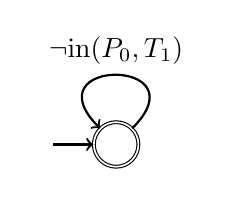
\begin{tikzpicture}
			\node[draw, circle, inner sep=0.2cm, double] (i) at (0,0) {};
			\draw[->, thick, loop] (i) to node[above] {$\neg \text{in}(P_0,T_1)$}(i); 
			\draw[->, thick] (-0.8,0) to (i); 
		\end{tikzpicture}
	\end{minipage}
	\hfill
	\begin{minipage}{0.22\textwidth}
		\centering
		complete \\
		\tiny
		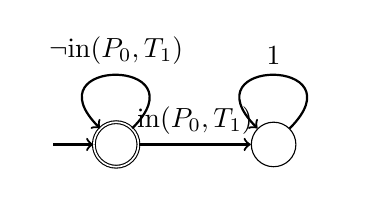
\begin{tikzpicture}
			\node[draw, circle, inner sep=0.2cm, double] (i) at (0,0) {};
			\node[draw, circle, inner sep=0.2cm] (d) at (2,0) {};
			\draw[->, thick, loop] (i) to node[above] {$\neg \text{in}(P_0,T_1)$} (i); 
			\draw[->, thick] (i) to node[above] {$\text{in}(P_0,T_1)$} (d);
			\draw[->, thick, loop] (d) to node[above] {$1$} (d); 
			\draw[->, thick] (-0.8,0) to (i); 
		\end{tikzpicture}
	\end{minipage}

\rebecca{the left automate creates a deadend in the compilation if $P_0$ is not in $T_1$ while the right does not.} 



% pgf settings: shrink the tick labels a bit
\pgfplotsset{every tick label/.append style={font=\scriptsize}}

\newcommand{\scatterplotsize}{8cm}
\newcommand{\scatterplotxlabelshift}{1.5ex}
\newcommand{\scatterplotylabelshift}{-3ex}




\section{Experiments}
\label{experiments}

%% \joerg{1.5--2 page: similar to ijcai version; expliucotly distinguish 
%% global vs local, add results for local in both ipc and action-set prop
%% experiments}

We implemented our approach in Fast Downward
(FD) \cite{helmert:jair-06}. We evaluate it, in turn, on IPC
benchmarks modified for OSP planning, and on a selection of IPC
benchmarks we extended with action-set properties.

The base planner called by our SysS and SysW algorithms on each search
node runs forward search using
\hff\ \cite{hoffmann:nebel:jair-01}, optionally with conjunction or trap learning.
%
%% The base planner configurations, used to solve/prove unsolvability
%% of a meta search node, are greedy best first search with $\hff$ and
%% preferred operators ($hff$) and conjunction learning $\hc$ with
%% $\hff$ as its base heuristic. \rebecca{ask Marcel how it is
%% called} \rebecca{Modification of hC to find deadends with an cost
%% bound}
%
The experiments were run on a cluster of Intel E5-2660 machines
running at 2.20 GHz, with time (memory) cut-offs of 30 minutes (4 GB).



 



%%%%%%%%%%%%%%%%%%%%%%%%%%%%%%%%%%%%%%%%%%%%%%%%%%%%%%%%%%%%%%%%%%%%
%%%%%%%%%%%%%%%%%%%%%%%%%%%%%%%%%%%%%%%%%%%%%%%%%%%%%%%%%%%%%%%%%%%%
%%%%%%%%%%%%%%%%%%%%%%%%%%%%%%%%%%%%%%%%%%%%%%%%%%%%%%%%%%%%%%%%%%%%
%%%% IPC OSP

\subsection{IPC-Based OSP Benchmarks}

% The net-benefit benchmarks don't give us anything new (the ones we
% could use are adopted from IPC ben chmarks anyhow).
%
%% \joerg{Rebecca/Michael: check out the IPC net-benefit benchmarks. Reviewers may naturally expect us to experiment with those, given our strong focus on oversubscription planning (actually this question came up in the discussion with the NASA guys yesterday). In the net-bnefit benchmarks, goal facts have rewards which we don't need. The question is whether, stripping away these rewards and imposing a plan-cost bound, we would get benchmarks not already covered by bour IPC experiments anyway. If the answer is "no", we can just say so in the paper. If the answer is "yes", it would be good (though probably not absolitely necessary) to experiment with these domains as well. In any case, we should know what the answer is.}

Following Katz et al.\ \shortcite{katz:etal:icaps-19}, for every IPC
benchmark task $(\vars,\acts,\cost,\init,\goal)$ with smallest known
plan cost $C$ as per planning.domains \cite{muise:icaps-demos-16}, we
obtained three OSP tasks by setting the cost bound to $b = x * C$
where $x \in \{0.25, 0.5, 0.75\}$. We used soft goals only, \ie,
$\goalsoft = \goal$ and $\goalhard=\emptyset$. For implementation
reasons, we omitted tasks with $\geq 32$ goals (which would be
infeasible for MUGS analysis anyhow).
%
%% ; the latter is an artifact of our current implementation that
%% could be overcome in principle, though computing all MUGS for that
%% many goals is presumably typically infeasible anyway.
%
% Joerg: said up front where it belongs
%
%% We extended conjunction learning \cite{steinmetz:hoffmann:ai-17} to
%% deal with cost bounds, thus enabling nogood learning and transfer in
%% SysS and SysW.
%
We consider conjunction learning, but not trap learning as that cannot
deal with OSP cost bounds.
%
%% In what follows, we consider first global explanations, then discuss
%% how the picture changes for local explanations.


\subsubsection{IPC Global Explanations}

\setlength{\tabcolsep}{2pt}
\renewcommand{\arraystretch}{0.8}
\begin{figure*}[h!]
\tiny
%\centering 	\tiny
	\begin{tabular}{l|rrr|rrr|rrr||rrr|rrr|rrr||rrr|rrr|rrr}
		& \multicolumn{9}{c||}{0.25} & \multicolumn{9}{c||}{0.5} & \multicolumn{9}{c}{0.75}\\
		& \multicolumn{3}{c|}{coverage} & \multicolumn{3}{c|}{avg time} & & & & \multicolumn{3}{c|}{covergae} & \multicolumn{3}{c|}{avg time} & & & & \multicolumn{3}{c|}{coverage} & \multicolumn{3}{c|}{avg time} & & &\\\hline
		& C & C nr & max & C & C nr & max & \#gs & \#n & fn & C & C nr & max & C & C nr & max & \#gs & \#n & fn & C & C nr & max & C & C nr & max & \#gs & \#n & fn\\\hline
		airport (28) & 0.93 & 0.93 & 0.86 & 0.0179 & 0.0296 & 15.5606 & 2.4 & 8.7 & 0.76 & 0.71 & 0.75 & 0.68 & 8.1089 & 3.8531 & 2.5639 & 1.9 & 4.4 & 0.71 & 0.57 & 0.57 & 0.68 & 3.4586 & 2.4734 & 0.256 & 1.0 & 2.4 & 0.61\\
		barman (4) & 1.00 & 1.00 & 1.00 & 0.003 & 0.0075 & 0.0382 & 3.0 & 7.0 & 0.88 & 1.00 & 1.00 & 1.00 & 42.121 & 26.4318 & 4.7071 & 3.0 & 7.0 & 0.88 & 0.00 & 0.00 & 1.00 & - & - & - & - & - & -\\
		blocks (28) & 1.00 & 0.93 & 0.96 & 0.0003 & 0.0006 & 0.0045 & 6.2 & 391.6 & 0.96 & 0.96 & 0.93 & 0.75 & 0.0006 & 0.0022 & 0.2815 & 6.6 & 138.7 & 0.93 & 0.89 & 0.86 & 0.61 & 0.0037 & 0.0072 & 0.7265 & 6.1 & 50.9 & 0.72\\
		data-net (12) & 0.00 & 0.00 & 1.00 & - & - & - & - & - & - & 0.00 & 0.00 & 1.00 & - & - & - & - & - & - & 0.00 & 0.00 & 1.00 & - & - & - & - & - & -\\
		depot (7) & 1.00 & 1.00 & 1.00 & 0.001 & 0.0027 & 0.065 & 4.0 & 36.1 & 0.94 & 1.00 & 1.00 & 1.00 & 1.2503 & 0.325 & 5.7004 & 7.0 & 34.6 & 0.91 & 0.43 & 0.43 & 0.57 & 4.9737 & 0.767 & 3.0968 & 2.7 & 11.0 & 0.68\\
		driverlog (13) & 1.00 & 1.00 & 1.00 & 0.0002 & 0.0007 & 0.0221 & 7.0 & 553.9 & 0.98 & 0.85 & 0.92 & 0.77 & 0.0062 & 0.0167 & 0.1872 & 13.4 & 387.4 & 0.86 & 0.69 & 0.69 & 0.62 & 2.4397 & 0.8843 & 4.7626 & 7.9 & 189.8 & 0.49\\
		elevators (40) & 0.00 & 0.00 & 1.00 &  &  &  &  &  &  & 0.00 & 0.00 & 1.00 & - & - & - & - & - & - & 0.00 & 0.00 & 0.83 & - & - & - & - & - & -\\
		floortile (13) & 0.54 & 0.46 & 0.46 & 0.0027 & 0.0077 & 0.0846 & 88.7 & 2881.7 & 0.99 & 0.15 & 0.15 & 0.15 & 0.4098 & 0.0973 & 0.3864 & 66.0 & 407.5 & 0.80 & 0.08 & 0.15 & 0.15 & 10.6455 & 2.4284 & 1.6908 & 30.0 & 142.0 & 0.28\\
		freecell (15) & 1.00 & 1.00 & 1.00 & 0.0007 & 0.004 & 0.1086 & 4.0 & 15.0 & 0.94 & 1.00 & 1.00 & 1.00 & 2.1944 & 0.3569 & 6.5571 & 4.7 & 15.0 & 0.94 & 0.87 & 0.87 & 0.93 & 3.5732 & 0.7317 & 24.2341 & 3.3 & 12.2 & 0.76\\
		ged (15) & 0.00 & 0.00 & 0.67 & - & - & - & - & - & - & 0.00 & 0.00 & 0.67 & - & - & - & - & - & - & 0.00 & 0.00 & 0.67 & - & - & - & - & - & -\\
		grid (2) & 1.00 & 1.00 & 1.00 & 0.0057 & 0.0068 & 0.0158 & 1.5 & 4.0 & 0.69 & 1.00 & 1.00 & 1.00 & 0.0131 & 0.0162 & 0.7963 & 1.5 & 4.0 & 0.69 & 1.00 & 1.00 & 1.00 & 0.1839 & 0.38 & 30.1363 & 1.0 & 3.0 & 0.56\\
		gripper (7) & 0.71 & 0.71 & 0.71 & 0.0036 & 0.0031 & 0.0089 & 77.4 & 1085.8 & 0.98 & 0.43 & 0.57 & 0.57 & 0.0547 & 0.0164 & 0.0076 & 32.0 & 97.0 & 0.89 & 0.43 & 0.43 & 0.71 & 0.7262 & 0.4556 & 0.0172 & 12.7 & 42.0 & 0.46\\
		hiking (9) & 1.00 & 1.00 & 1.00 & 0.0078 & 0.0079 & 0.1617 & 1.4 & 1.9 & 0.61 & 1.00 & 1.00 & 1.00 & 10.1549 & 4.5974 & 2.5455 & 1.4 & 1.9 & 0.61 & 1.00 & 1.00 & 1.00 & 173.4486 & 105.979 & 3.7597 & 1.0 & 1.9 & 0.61\\
		logistics (26) & 1.00 & 1.00 & 0.85 & 0.0006 & 0.0018 & 2.5104 & 4.6 & 108.1 & 0.95 & 0.77 & 0.85 & 0.58 & 0.0732 & 0.0309 & 2.7788 & 4.6 & 47.2 & 0.84 & 0.54 & 0.58 & 0.46 & 0.2428 & 0.0851 & 0.1558 & 2.2 & 20.5 & 0.63\\
		miconic (141) & 0.45 & 0.46 & 0.40 & 0.0022 & 0.0033 & 0.0261 & 27.9 & 436.3 & 0.91 & 0.28 & 0.35 & 0.32 & 0.0778 & 0.0119 & 0.0405 & 16.3 & 55.2 & 0.82 & 0.25 & 0.28 & 0.32 & 0.5958 & 0.0925 & 0.0495 & 5.5 & 18.7 & 0.61\\
		movie (30) & 1.00 & 1.00 & 1.00 & 0.0001 & 0.0001 & 0.0001 & 7.0 & 127.0 & 0.99 & 1.00 & 1.00 & 1.00 & 0.0008 & 0.0011 & 0.0003 & 35.0 & 120.0 & 0.94 & 1.00 & 1.00 & 1.00 & 0.0086 & 0.0114 & 0.0013 & 21.0 & 64.0 & 0.50\\
		mprime (22) & 1.00 & 1.00 & 1.00 & 0.0076 & 0.0081 & 0.0206 & 1.3 & 1.7 & 0.59 & 1.00 & 1.00 & 1.00 & 0.0079 & 0.009 & 0.354 & 1.2 & 1.7 & 0.59 & 1.00 & 1.00 & 1.00 & 0.0188 & 0.0235 & 13.4521 & 1.2 & 1.7 & 0.59\\
		mystery (17) & 1.00 & 1.00 & 1.00 & 0.0068 & 0.0083 & 0.039 & 1.4 & 2.2 & 0.63 & 1.00 & 1.00 & 1.00 & 0.0076 & 0.0111 & 1.7946 & 1.4 & 2.2 & 0.63 & 1.00 & 1.00 & 0.88 & 0.0085 & 0.0141 & 1.6148 & 1.2 & 2.2 & 0.63\\
		nomystery (14) & 1.00 & 1.00 & 1.00 & 0.0007 & 0.0032 & 0.062 & 7.3 & 144.1 & 0.96 & 0.86 & 0.86 & 0.71 & 0.1669 & 0.0289 & 1.9467 & 12.8 & 46.0 & 0.92 & 0.57 & 0.57 & 0.57 & 1.9144 & 0.363 & 2.3241 & 5.8 & 17.8 & 0.61\\
		openstacks (47) & 0.15 & 0.15 & 0.51 & 0.0011 & 0.0112 & 0.0709 & 6.4 & 314.4 & 0.98 & 0.11 & 0.11 & 0.47 & 0.0087 & 0.0179 & 0.0091 & 4.6 & 30.8 & 0.96 & 0.11 & 0.11 & 0.43 & 0.4592 & 0.4069 & 0.0198 & 5.2 & 29.2 & 0.91\\
		organic-syn (7) & 1.00 & 0.86 & 0.86 & 0.0004 & 0.0142 & 0.0577 & 4.0 & 38.3 & 0.93 & 1.00 & 0.86 & 0.86 & 0.0017 & 0.0193 & 0.0586 & 4.0 & 38.3 & 0.93 & 1.00 & 0.86 & 0.86 & 0.002 & 0.0224 & 0.0561 & 4.0 & 38.3 & 0.93\\
		organic-syn-s (10) & 0.80 & 0.60 & 0.60 & 0.0005 & 0.011 & 3.3391 & 4.0 & 62.0 & 0.95 & 0.80 & 0.50 & 0.60 & 0.0003 & 0.0059 & 0.0305 & 4.0 & 68.2 & 0.94 & 0.50 & 0.50 & 0.60 & 0.0334 & 0.6536 & 0.0416 & 4.0 & 66.6 & 0.89\\
		parcprinter (24) & 0.00 & 0.00 & 0.42 & - & - & - & - & - & - & 0.00 & 0.00 & 0.42 & - & - & - & - & - & - & 0.00 & 0.00 & 0.42 & - & - & - & - & - & -\\
		parking (5) & 1.00 & 0.00 & 0.00 & - & - & - & - & - & - & 0.00 & 0.00 & 0.00 & - & - & - & - & - & - & 0.00 & 0.00 & 0.00 & - & - & - & - & - & -\\
		pathways-n (5) & 1.00 & 1.00 & 1.00 & 0.0032 & 0.0034 & 0.8366 & 3.2 & 17.8 & 0.81 & 1.00 & 1.00 & 0.80 & 0.0039 & 0.0047 & 0.021 & 2.3 & 6.5 & 0.77 & 0.80 & 0.80 & 0.80 & 0.0101 & 0.0129 & 0.0675 & 1.8 & 6.0 & 0.70\\
		pegsol (2) & 0.00 & 0.00 & 0.00 & - & - & - & - & - & - & 0.00 & 0.00 & 0.00 & - & - & - & - & - & - & 0.00 & 0.00 & 0.00 & - & - & - & - & - & -\\
		pipesworld-nt (17) & 1.00 & 1.00 & 1.00 & 0.0013 & 0.0032 & 0.0284 & 3.7 & 38.7 & 0.89 & 1.00 & 1.00 & 0.94 & 0.639 & 0.3373 & 1.2171 & 4.8 & 23.5 & 0.84 & 0.82 & 0.82 & 0.94 & 8.308 & 8.7389 & 28.7631 & 4.1 & 17.4 & 0.66\\
		pipesworld-t (12) & 1.00 & 1.00 & 1.00 & 0.0017 & 0.0096 & 0.1815 & 3.6 & 34.7 & 0.94 & 0.92 & 0.92 & 0.92 & 0.1758 & 0.1562 & 6.1596 & 5.0 & 29.7 & 0.87 & 0.67 & 0.75 & 0.75 & 0.3663 & 0.3553 & 9.9122 & 3.1 & 14.0 & 0.63\\
		psr (49) & 1.00 & 0.98 & 0.98 & 0.0014 & 0.0016 & 0.0017 & 3.5 & 614.0 & 0.63 & 1.00 & 0.98 & 0.98 & 0.0016 & 0.0027 & 0.004 & 2.5 & 473.6 & 0.55 & 0.98 & 0.94 & 0.96 & 0.0059 & 0.0108 & 0.0836 & 1.8 & 80.0 & 0.47\\
		rovers (8) & 1.00 & 1.00 & 1.00 & 0.0054 & 0.002 & 0.045 & 18.0 & 161.4 & 0.93 & 0.88 & 0.88 & 0.88 & 0.4482 & 0.04 & 0.9443 & 11.4 & 33.0 & 0.84 & 0.63 & 0.88 & 0.75 & 10.5432 & 4.1379 & 2.2399 & 2.2 & 8.6 & 0.55\\
		satellite (7) & 1.00 & 1.00 & 1.00 & 0.0004 & 0.0014 & 0.1674 & 5.6 & 173.9 & 0.97 & 1.00 & 1.00 & 0.86 & 0.0199 & 0.0214 & 0.6192 & 18.7 & 112.5 & 0.94 & 0.71 & 0.86 & 0.57 & 0.1161 & 0.0451 & 0.0826 & 13.3 & 49.8 & 0.73\\
		scanalyzer (23) & 0.57 & 0.39 & 0.39 & 0.0001 & 0.0007 & 0.0061 & 12.9 & 2357.3 & 0.99 & 0.39 & 0.39 & 0.39 & 0.0348 & 0.0097 & 0.08 & 45.8 & 1937.8 & 0.86 & 0.22 & 0.22 & 0.39 & 0.1143 & 0.0165 & 0.0742 & 30.8 & 549.2 & 0.83\\
		snake (7) & 0.86 & 0.14 & 0.14 & 0.0006 & 0.014 & 0.244 & 6.0 & 244.0 & 0.95 & 0.43 & 0.14 & 0.14 & 0.0051 & 0.0301 & 0.2366 & 11.0 & 234.0 & 0.91 & 0.14 & 0.00 & 0.14 & - & - & - & - & - & -\\
		sokoban (50) & 0.00 & 0.00 & 0.98 & - & - & - & - & - & - & 0.00 & 0.00 & 0.94 & - & - & - & - & - & - & 0.00 & 0.00 & 0.84 & - & - & - & - & - & -\\
		storage (15) & 1.00 & 1.00 & 1.00 & 0.0032 & 0.0034 & 0.0047 & 3.6 & 11.4 & 0.81 & 1.00 & 1.00 & 1.00 & 0.1895 & 0.0394 & 0.0953 & 3.7 & 10.1 & 0.75 & 0.93 & 0.93 & 1.00 & 9.2279 & 2.4855 & 0.536 & 1.9 & 5.7 & 0.57\\
		termes (6) & 1.00 & 0.33 & 1.00 & 0.0005 & 0.0203 & 0.0193 & 2.5 & 2880.0 & 0.70 & 0.33 & 0.00 & 0.17 & - & - & - & - & - & - & 0.00 & 0.00 & 0.00 & - & - & - & - & - & -\\
		tetris (6) & 0.83 & 0.33 & 0.33 & 0.0002 & 0.0063 & 0.0146 & 6.5 & 255.0 & 1.00 & 0.50 & 0.33 & 0.33 & 0.0074 & 0.0152 & 0.0243 & 10.0 & 204.0 & 0.80 & 0.33 & 0.33 & 0.50 & 0.6283 & 0.2585 & 0.0736 & 5.5 & 104.5 & 0.41\\
		tidybot (23) & 1.00 & 1.00 & 1.00 & 0.0039 & 0.0462 & 1.7383 & 3.1 & 14.7 & 0.92 & 0.96 & 0.96 & 1.00 & 3.3049 & 2.1666 & 23.4994 & 3.1 & 14.7 & 0.92 & 0.52 & 0.35 & 0.30 & 7.0445 & 6.7422 & 8.1621 & 3.5 & 13.7 & 0.85\\
		tpp (7) & 1.00 & 1.00 & 1.00 & 0.0023 & 0.0027 & 0.0145 & 4.1 & 35.3 & 0.86 & 0.86 & 1.00 & 0.86 & 0.0271 & 0.0111 & 0.1495 & 6.2 & 19.3 & 0.83 & 0.71 & 0.86 & 0.86 & 0.023 & 0.014 & 0.0102 & 2.8 & 7.6 & 0.66\\
		transport (23) & 1.00 & 1.00 & 1.00 & 0.0011 & 0.0015 & 0.0103 & 3.3 & 15.5 & 0.91 & 1.00 & 1.00 & 1.00 & 0.0429 & 0.0536 & 0.5756 & 3.4 & 14.8 & 0.88 & 0.96 & 0.96 & 1.00 & 5.0431 & 2.1916 & 8.1134 & 2.2 & 10.6 & 0.68\\
		trucks (10) & 1.00 & 1.00 & 1.00 & 0.0042 & 0.0146 & 0.4801 & 15.7 & 145.4 & 0.97 & 0.70 & 0.90 & 0.60 & 0.9799 & 0.0891 & 1.225 & 14.8 & 46.5 & 0.89 & 0.30 & 0.40 & 0.60 & 1.5139 & 0.3479 & 0.0774 & 3.7 & 11.0 & 0.65\\
		visitall (14) & 0.71 & 0.57 & 0.64 & 0.0016 & 0.0016 & 0.0017 & 20.1 & 10289.6 & 0.91 & 0.71 & 0.50 & 0.57 & 0.0019 & 0.0023 & 0.0041 & 38.0 & 6928.6 & 0.89 & 0.57 & 0.50 & 0.50 & 0.0044 & 0.0054 & 0.0189 & 38.3 & 4532.0 & 0.74\\
		woodworking (29) & 0.52 & 0.17 & 0.24 & 0.0001 & 0.0004 & 0.0014 & 20.0 & 2147.0 & 1.00 & 0.31 & 0.17 & 0.17 & 0.0011 & 0.0032 & 0.0078 & 33.8 & 1975.0 & 0.93 & 0.17 & 0.17 & 0.17 & 0.0144 & 0.0341 & 0.0485 & 16.8 & 1087.4 & 0.52\\
		zenotravel (13) & 1.00 & 1.00 & 0.92 & 0.0008 & 0.0034 & 0.1252 & 8.3 & 120.8 & 0.94 & 0.69 & 0.77 & 0.62 & 0.0011 & 0.0026 & 0.0228 & 3.8 & 36.6 & 0.89 & 0.69 & 0.69 & 0.62 & 0.4387 & 0.1626 & 0.8227 & 2.4 & 25.3 & 0.66\\\hline
		Sum (862) & 0.65 & 0.60 & 0.76 & 0.0026 & 0.0072 & 0.7059 & 10.9 & 696.7 & 0.88 & 0.55 & 0.55 & 0.68 & 1.9595 & 1.0787 & 1.8231 & 12.2 & 378.0 & 0.84 & 0.46 & 0.46 & 0.62 & 7.2394 & 4.157 & 4.2789 & 7.3 & 212.9 & 0.64\\\hline\hline
		nomystery (13, 25, 25) & 14 & 14 & 14 & 0.0004 & 0.0021 & 0.0262 & 8.6 & 507 & - & 21 & 22 & 2 & 0.0015 & 0.0132 & 0.2042 & 14 & 511 & - & 4 & 0 & 0 & - & - & - & - & - & - \\ 
		rovers (10, 25, 25) & 12 & 0 & 0 & - &  - & - & - & - & - & 8 & 0 & 0 &  - & - & - & - & - & - & 0 & 0 & 0 & - & - & - & - & - & - \\
		tpp (5) & 5 & 5 & 5 & 0.0279 & 0.2685 & 0.4789 & - & - & - &  1 & 0 & 0 & - & - & - & - & - & - & 0 & 0 & 0 & - & - & - & - & - & - \\

	\end{tabular}


%
\centering % 3 * 5 coverage, 3 * goal size, 3 * 2 fraction search tree
\begin{tabular}{l||r|rrr||rrrr|rrrr|rrrr||rr|rr|rr||rrr|rrr}
& \multicolumn{4}{c||}{Reference Coverage}  & \multicolumn{12}{c||}{Systematic Strengthening/Weakening Coverage, $x=$} & \multicolumn{6}{c||}{Search Tree Fraction, $x=$} & \multicolumn{6}{c}{\#MUGS, $x=$} \\
& \hlmcut & \multicolumn{3}{c||}{OSP} & \multicolumn{4}{c|}{0.25} & \multicolumn{4}{c|}{0.5} & \multicolumn{4}{c||}{0.75} & \multicolumn{2}{c|}{0.25} & \multicolumn{2}{c|}{0.5} & \multicolumn{2}{c||}{0.75} & 0.25 & 0.5 & 0.75 & 0.25 & 0.5 & 0.75 \\\hline
& & \multicolumn{3}{c||}{$x=$} & \multicolumn{2}{c}{SysS} & \multicolumn{2}{c|}{SysW}& \multicolumn{2}{c}{SysS} & \multicolumn{2}{c|}{SysW}& \multicolumn{2}{c}{SysS} & \multicolumn{2}{c||}{SysW} &\multicolumn{2}{c|}{Sys} & \multicolumn{2}{c|}{Sys} & \multicolumn{2}{c||}{Sys} & & & & & &  \\
domain               &    &0.25& 0.5&0.75&    &\hc &    &\hc &    &\hc &    &\hc &    &\hc &    &\hc &    S &    W &    S &    W &    S &    W & \multicolumn{3}{c|}{average} & \multicolumn{3}{c}{max} \\\hline\hline
agricola (20)         & 0 & 0 & 0 & 0 & \textbf{20}  & \textbf{20}  & \textbf{20}  & \textbf{20}  & 12 & \textbf{13}  & 11 & \textbf{13}  &  \textbf{2}  & 1 &  \textbf{2}  & 1 & 1.00 & \textbf{0.50}  & 1.00 & \textbf{0.50}  & 1.00 & \textbf{0.50}  & 1.0 & 1.0 & 1.0 & 1 & 1 & 1 \\
airport (50)          & 28 & 28 & 24 & 22 & 25 & \textbf{35}  & 24 & 34 & 20 & \textbf{21}  & 19 & \textbf{21}  & \textbf{20}  & 16 & \textbf{20}  & 16 & \textbf{0.60}  & 0.81 & 0.87 & \textbf{0.73}  & 1.00 & \textbf{0.61}  & 3.8 & 2.0 & 1.4 & 16 & 5 & 4 \\
barman (34)           & 4 & 18 & 11 & 4 & \textbf{18}  & \textbf{18}  & 15 & \textbf{18}  & \textbf{11}  & 4 & 10 & 4 &  \textbf{8}  & 3 & 7 & 4 & \textbf{0.57}  & 0.94 & \textbf{0.88}  & \textbf{0.88}  & 1.00 & \textbf{0.50}  & 6.9 & 4.2 & 2.5 & 10 & 6 & 4 \\
blocks (35)           & 28 & 35 & 28 & 21 & \textbf{35}  & \textbf{35}  & 29 & \textbf{35}  & 25 & \textbf{29}  & 22 & \textbf{29}  & 18 & \textbf{26}  & 18 & \textbf{26}  & \textbf{0.15}  & 0.97 & \textbf{0.35}  & 0.95 & 0.80 & \textbf{0.64}  & 11.0 & 12.4 & 13.7 & 59 & 40 & 57 \\
childsnack (20)       & 0 & 2 & 0 & 0 & 0 &  \textbf{4}  & 0 &  \textbf{4}  & 0 & 0 & 0 & 0 & 0 & 0 & 0 & 0 & \textbf{0.34}  & 0.98 &    -    &   -     &   -     &    -    & 16.8 &   -     &  -  & 20 & -   &  -  \\
data-network (20)     & 12 & 13 & 13 & 13 & 19 & \textbf{20}  & 19 & \textbf{20}  & 17 & \textbf{18}  & 16 & \textbf{18}  & 13 & \textbf{17}  & 13 & 15 & \textbf{0.72}  & 0.73 & 0.79 & \textbf{0.70}  & 0.91 & \textbf{0.66}  & 2.1 & 1.8 & 1.5 & 4 & 3 & 3 \\
depot (22)            & 7 & 16 & 11 & 7 & 15 & \textbf{16}  & 12 & \textbf{16}  & 7 & 9 & 7 & \textbf{10}  &  \textbf{6}  & 3 &  \textbf{6}  & 3 & \textbf{0.24}  & 0.96 & \textbf{0.54}  & 0.90 & 0.89 & \textbf{0.68}  & 8.3 & 7.0 & 6.5 & 29 & 13 & 15 \\
driverlog (20)        & 13 & 15 & 13 & 10 & \textbf{15}  & \textbf{15}  & \textbf{15}  & \textbf{15}  & 11 & \textbf{12}  & 11 & \textbf{12}  & 9 & \textbf{10}  & 9 & \textbf{10}  & \textbf{0.17}  & 0.98 & \textbf{0.59}  & 0.86 & 0.87 & \textbf{0.50}  & 8.1 & 16.1 & 11.1 & 18 & 45 & 21 \\
elevators (50)        & 40 & 22 & 22 & 22 & \textbf{49}  & 47 & \textbf{49}  & 48 & \textbf{44}  & 38 & 43 & 37 & \textbf{43}  & 27 & 41 & 27 & \textbf{0.35}  & 0.94 & \textbf{0.67}  & 0.89 & 0.90 & \textbf{0.67}  & 4.6 & 5.1 & 5.9 & 14 & 12 & 21 \\
floortile (36)        & 13 & 18 & 6 & 2 & \textbf{15}  & 8 & 6 & 8 &  \textbf{3}  & 2 & 2 & 2 &  \textbf{2}  &  \textbf{2}  &  \textbf{2}  &  \textbf{2}  & \textbf{0.10}  & 0.99 & \textbf{0.67}  & 0.80 & 0.96 & \textbf{0.30}  & 316.2 & 137.0 & 45.5 & 622 & 321 & 54 \\
freecell (80)         & 15 & 77 & 30 & 21 & 51 & \textbf{76}  & 41 & \textbf{76}  & 25 & \textbf{30}  & 21 & \textbf{30}  & 15 & \textbf{18}  & 15 & \textbf{18}  & \textbf{0.31}  & 0.94 & \textbf{0.62}  & 0.94 & 0.88 & \textbf{0.76}  & 4.0 & 4.3 & 3.3 & 4 & 6 & 5 \\
ged (20)              & 15 & 20 & 20 & 20 & 16 & 16 & 15 & \textbf{20}  & \textbf{15}  & 10 & 10 & 12 & \textbf{10}  & 7 & \textbf{10}  & 7 & \textbf{0.25}  & 0.90 & \textbf{0.47}  & 0.80 & \textbf{0.58}  & 0.70 & 13.3 & 38.7 & 12.5 & 30 & 101 & 38 \\
grid (5)              & 2 & 5 & 3 & 2 & 4 &  \textbf{5}  & 4 &  \textbf{5}  & 3 & 3 & 3 &  \textbf{4}  & 2 &  \textbf{3}  & 2 &  \textbf{3}  & \textbf{0.54}  & 0.84 & 0.83 & \textbf{0.75}  & 1.00 & \textbf{0.54}  & 4.0 & 2.5 & 1.0 & 7 & 4 & 1 \\
gripper (20)          & 7 & 11 & 8 & 8 &  \textbf{8}  & 5 & 6 & 5 &  \textbf{5}  & 4 &  \textbf{5}  & 4 &  \textbf{5}  & 3 &  \textbf{5}  & 3 & \textbf{0.21}  & 0.98 & \textbf{0.65}  & 0.88 & 0.96 & \textbf{0.46}  & 783.5 & 228.0 & 156.0 & 3060 & 792 & 495 \\
hiking (20)           & 9 & 19 & 14 & 13 & 19 & \textbf{20}  & 19 & \textbf{20}  & 14 & 16 & 13 & \textbf{17}  & \textbf{14}  & 11 & 13 & 10 & 0.81 & \textbf{0.69}  & 0.83 & \textbf{0.67}  & 1.00 & \textbf{0.63}  & 1.8 & 1.7 & 1.0 & 2 & 2 & 1 \\
logistics (60)        & 26 & 27 & 20 & 16 & 7 & \textbf{15}  & 6 & \textbf{15}  & 4 &  \textbf{6}  & 4 &  \textbf{6}  & 3 & 3 & 3 &  \textbf{4}  & \textbf{0.35}  & 0.95 & \textbf{0.73}  & 0.81 & 0.98 & \textbf{0.73}  & 7.2 & 7.3 & 2.8 & 18 & 22 & 4 \\
miconic (150)         & 141 & 97 & 66 & 55 & \textbf{75}  & 66 & 60 & 64 & \textbf{51}  & 42 & 47 & 43 & \textbf{45}  & 35 & \textbf{45}  & 36 & \textbf{0.30}  & 0.92 & \textbf{0.73}  & 0.82 & 0.95 & \textbf{0.61}  & 81.3 & 38.2 & 18.8 & 452 & 285 & 98 \\
mprime (35)           & 22 & 35 & 27 & 24 & \textbf{35}  & \textbf{35}  & 35 & \textbf{35}  & 28 & \textbf{35}  & 28 & \textbf{35}  & 25 & \textbf{35}  & 24 & \textbf{35}  & 0.90 & \textbf{0.59}  & 0.91 & \textbf{0.59}  & 0.94 & \textbf{0.59}  & 1.3 & 1.2 & 1.1 & 2 & 2 & 2 \\
mystery (30)          & 12 & 29 & 27 & 21 & \textbf{30}  & \textbf{30}  & \textbf{30}  & \textbf{30}  & \textbf{30}  & \textbf{30}  & 29 & \textbf{30}  & 21 & \textbf{30}  & 20 & \textbf{30}  & 0.89 & \textbf{0.61}  & 0.90 & \textbf{0.61}  & 0.93 & \textbf{0.61}  & 1.3 & 1.2 & 1.1 & 2 & 2 & 2 \\
nomystery (20)        & 14 & 20 & 14 & 10 & \textbf{20}  & \textbf{20}  & 16 & \textbf{20}  & 10 & \textbf{12}  & 10 & \textbf{12}  &  \textbf{8}  &  \textbf{8}  &  \textbf{8}  &  \textbf{8}  & \textbf{0.15}  & 0.98 & \textbf{0.61}  & 0.92 & 0.87 & \textbf{0.61}  & 20.2 & 18.5 & 5.8 & 61 & 47 & 13 \\
openstacks (77)       & 47 & 63 & 56 & 52 & \textbf{49}  & \textbf{49}  & 37 & 43 & \textbf{47}  & 45 & 29 & 39 & \textbf{42}  & \textbf{42}  & 24 & 35 & \textbf{0.03}  & 0.99 & \textbf{0.04}  & 0.99 & \textbf{0.12}  & 0.98 & 15.3 & 14.9 & 10.3 & 25 & 44 & 23 \\
organic-syn-s (13)    & 10 & 8 & 8 & 8 &  \textbf{8}  &  \textbf{8}  & 7 &  \textbf{8}  &  \textbf{8}  &  \textbf{8}  & 7 &  \textbf{8}  &  \textbf{7}  & 6 & 6 & 6 & \textbf{0.19}  & 0.96 & \textbf{0.21}  & 0.95 & \textbf{0.28}  & 0.91 & 5.3 & 7.3 & 8.3 & 12 & 28 & 36 \\
parcprinter (26)      & 24 & 26 & 22 & 18 & 10 & 10 & 12 & \textbf{14}  & 10 & 10 & 10 & \textbf{14}  & 10 & 10 & 10 & \textbf{12}  & \textbf{0.44}  & 0.98 & \textbf{0.61}  & 0.95 & \textbf{0.73}  & 0.85 & 5.6 & 7.5 & 4.1 & 14 & 24 & 8 \\
parking (40)          & 5 & 25 & 5 & 0 & 12 & \textbf{17}  & 5 & 12 & 0 &  \textbf{1}  & 0 &  \textbf{1}  & 0 & 0 & 0 & 0 & \textbf{0.02}  & 1.00 & \textbf{0.27}  & 0.91 &  -      &  -      & 63.9 & 31.0 &    & 112 & 31 &  -  \\
pathways (30)         & 5 & 5 & 4 & 4 & 5 &  \textbf{7}  & 5 &  \textbf{7}  & 4 &  \textbf{5}  & 4 &  \textbf{5}  &  \textbf{4}  &  \textbf{4}  &  \textbf{4}  &  \textbf{4}  & \textbf{0.41}  & 0.86 & \textbf{0.72}  & 0.78 & 0.91 & \textbf{0.70}  & 11.3 & 3.8 & 1.8 & 50 & 10 & 3 \\
pegsol (2)            & 2 & 2 & 2 & 2 & 0 & 0 &  \textbf{2}  &  \textbf{2}  & 0 & 0 &  \textbf{2}  &  \textbf{2}  & 0 & 0 &  \textbf{2}  &  \textbf{2}  &   -     &   -     &   -     &    -    &   -     &   -     & 7.0 & 23.5 & 64.0 & 8 & 41 & 122 \\
pipesworld-nt (50)    & 17 & 45 & 30 & 23 & 42 & \textbf{46}  & 38 & \textbf{46}  & \textbf{26}  & 25 & 24 & \textbf{26}  & \textbf{21}  & 15 & 20 & 15 & \textbf{0.31}  & 0.94 & \textbf{0.68}  & 0.83 & 0.88 & \textbf{0.66}  & 5.0 & 5.6 & 4.3 & 13 & 31 & 24 \\
pipesworld-t (50)     & 12 & 33 & 20 & 16 & 23 & 39 & 20 & \textbf{40}  & 14 & \textbf{18}  & 13 & 17 & 11 & \textbf{13}  & 9 & 11 & \textbf{0.35}  & 0.95 & \textbf{0.63}  & 0.86 & 0.88 & \textbf{0.65}  & 4.0 & 4.2 & 3.2 & 12 & 15 & 12 \\
psr-small (50)        & 49 & 50 & 50 & 50 & 48 & 48 & 49 & \textbf{50}  & 47 & 47 & 48 & \textbf{49}  & 46 & 46 & \textbf{48}  & \textbf{48}  & 0.76 & \textbf{0.63}  & 0.94 & \textbf{0.55}  & 0.97 & \textbf{0.47}  & 4.0 & 2.7 & 2.0 & 20 & 13 & 11 \\
rovers (40)           & 8 & 16 & 8 & 6 & \textbf{12}  & \textbf{12}  & \textbf{12}  & \textbf{12}  &  \textbf{7}  &  \textbf{7}  &  \textbf{7}  &  \textbf{7}  &  \textbf{7}  & 5 &  \textbf{7}  & 5 & \textbf{0.31}  & 0.95 & \textbf{0.74}  & 0.84 & 0.92 & \textbf{0.55}  & 21.0 & 11.4 & 4.3 & 95 & 35 & 12 \\
satellite (36)        & 7 & 9 & 7 & 6 & 9 & \textbf{12}  & 7 & \textbf{12}  & 6 & 6 & 6 &  \textbf{7}  &  \textbf{6}  & 5 &  \textbf{6}  &  \textbf{6}  & \textbf{0.12}  & 0.98 & \textbf{0.49}  & 0.94 & 0.90 & \textbf{0.68}  & 31.1 & 23.3 & 20.5 & 136 & 76 & 56 \\
scanalyzer (40)       & 23 & 26 & 21 & 21 & 9 & \textbf{17}  & 9 & 15 &  \textbf{9}  &  \textbf{9}  &  \textbf{9}  &  \textbf{9}  &  \textbf{9}  & 5 &  \textbf{9}  &  \textbf{9}  & \textbf{0.22}  & 0.99 & \textbf{0.53}  & 0.86 & \textbf{0.75}  & 0.83 & 35.2 & 37.8 & 62.6 & 106 & 71 & 130 \\
snake (17)            & 6 & 17 & 17 & 14 &  \textbf{7}  &  \textbf{7}  & 6 &  \textbf{7}  &  \textbf{3}  &  \textbf{3}  &  \textbf{3}  &  \textbf{3}  &  \textbf{3}  & 1 &  \textbf{3}  & 1 & \textbf{0.16}  & 0.93 & \textbf{0.32}  & 0.86 & \textbf{0.58}  & 0.74 & 11.4 & 20.3 & 38.3 & 17 & 25 & 59 \\
sokoban (50)          & 49 & 50 & 49 & 45 & \textbf{50}  & \textbf{50}  & 49 & \textbf{50}  & \textbf{48}  & 43 & \textbf{48}  & 43 & \textbf{44}  & 31 & \textbf{44}  & 29 & \textbf{0.59}  & 0.85 & 0.86 & \textbf{0.72}  & 0.96 & \textbf{0.49}  & 4.9 & 4.0 & 2.2 & 56 & 32 & 14 \\
spider (12)           &  11    & 12 & 12 & 12 &  \textbf{6}  &  \textbf{6}  & 1 & 1 &  \textbf{5}  & 1 & 0 & 0 & 0 & 0 & 0 & 0 &   0.00     &   1.00     &   -     &   -     &   -     &    -    & 21.0 & 32.4 & 2.3 & 36 & 57 & -   \\
storage (30)          & 15 & 20 & 17 & 15 & \textbf{18}  & \textbf{18}  & \textbf{18}  & \textbf{18}  & \textbf{16}  & \textbf{16}  & \textbf{16}  & \textbf{16}  & \textbf{15}  & 14 & \textbf{15}  & 14 & \textbf{0.57}  & 0.83 & 0.85 & \textbf{0.75}  & 0.98 & \textbf{0.57}  & 5.0 & 4.3 & 8.9 & 15 & 11 & 5 \\
termes (20)           & 6 & 20 & 16 & 12 & \textbf{20}  & 11 & 13 & 10 & \textbf{15}  & 2 & 3 & 3 &  \textbf{7}  & 0 & 1 & 0 & \textbf{0.28}  & 0.80 & \textbf{0.53}  & \textbf{0.53}  & -     &  -      & 3.8 & 6.0 &  -  & 10 & 18 & 24 \\
tetris (17)           & 6 & 17 & 14 & 11 & 8 &  \textbf{9}  & 7 & 7 &  \textbf{5}  & 3 & 3 & 3 &  \textbf{3}  & 2 &  \textbf{3}  & 2 & \textbf{0.23}  & 0.98 & 0.81 & \textbf{0.77}  & 0.97 & \textbf{0.41}  & 38.2 & 43.8 & 7.3 & 79 & 89 & 11 \\
tidybot (40)          & 23 & 40 & 38 & 32 & \textbf{40}  & \textbf{40}  & 39 & \textbf{40}  & \textbf{32}  & 31 & 25 & 28 & \textbf{14}  & 13 & 8 & \textbf{14}  & \textbf{0.38}  & 0.92 & \textbf{0.47}  & 0.91 & \textbf{0.69}  & 0.79 & 3.1 & 3.3 & 2.9 & 4 & 6 & 6 \\
tpp (30)              & 7 & 9 & 7 & 6 & 8 &  \textbf{9}  & 8 &  \textbf{9}  &  \textbf{7}  &  \textbf{7}  & 6 &  \textbf{7}  &  \textbf{6}  & 5 &  \textbf{6}  & 5 & \textbf{0.36}  & 0.89 & \textbf{0.66}  & 0.82 & 0.96 & \textbf{0.66}  & 8.0 & 8.9 & 4.2 & 33 & 25 & 11 \\
transport (70)        & 23 & 24 & 24 & 24 & \textbf{42}  & \textbf{42}  & 37 & \textbf{42}  & \textbf{34}  & \textbf{34}  & \textbf{34}  & 33 & 31 & 23 & \textbf{33}  & 26 & \textbf{0.37}  & 0.94 & \textbf{0.59}  & 0.89 & 0.73 & \textbf{0.69}  & 5.3 & 4.1 & 2.7 & 22 & 10 & 10 \\
trucks (30)           & 10 & 12 & 8 & 6 & 12 & \textbf{14}  & 9 & \textbf{14}  &  \textbf{7}  &  \textbf{7}  & 6 &  \textbf{7}  &  \textbf{6}  & 4 & 6 & 4 & \textbf{0.18}  & 0.98 & \textbf{0.68}  & 0.89 & 0.93 & \textbf{0.62}  & 30.2 & 17.4 & 7.7 & 137 & 32 & 21 \\
visitall (14)         & 14 & 14 & 14 & 13 & \textbf{13}  & \textbf{13}  & 10 & 10 & \textbf{10}  & \textbf{10}  & 8 & \textbf{10}  & 6 & 6 & 7 &  \textbf{8}  & \textbf{0.20}  & 0.93 & \textbf{0.36}  & 0.91 & 0.79 & \textbf{0.75}  & 99.6 & 166.0 & 115.1 & 313 & 602 & 466 \\
woodworking (35)      & 29 & 25 & 12 & 10 & \textbf{23}  & \textbf{23}  & 13 & 15 &  \textbf{9}  &  \textbf{9}  & 7 &  \textbf{9}  &  \textbf{5}  &  \textbf{5}  &  \textbf{5}  &  \textbf{5}  & \textbf{0.02}  & 1.00 & \textbf{0.22}  & 0.94 & 0.72 & \textbf{0.52}  & 198.0 & 95.1 & 19.8 & 532 & 182 & 28 \\
zenotravel (20)       & 13 & 13 & 10 & 8 & \textbf{13}  & \textbf{13}  & 12 & \textbf{13}  & \textbf{10}  & 9 & 8 & 9 & 8 &  \textbf{9}  & 8 &  \textbf{9}  & \textbf{0.34}  & 0.94 & \textbf{0.65}  & 0.88 & 0.86 & \textbf{0.64}  & 10.5 & 6.7 & 2.6 & 36 & 31 & 4 \\\hline
Sum (1517)            & 828 & 1088 & 828 & 705 & 963 & \textbf{1026}  & 846 & 1005 & \textbf{714}  & 690 & 637 & 694 & \textbf{580}  & 522 & 547 & 528 &    &    &    &    &    &    &    &    &    &    &    &    \\
\end{tabular}

%% agricola (20)        &  0 &  0 &  0 &  0 &\textbf{20} &\textbf{20} &\textbf{20} &\textbf{20} & 11 &\textbf{13} & 12 &\textbf{13} & \textbf{2} &  1 & \textbf{2} &  1 & 1.00 &\textbf{0.50} & 1.00 &\textbf{0.50} & 1.00 &\textbf{0.50} & 1.0 & 1.0 & 1.0 &  1 &  1 &  1 \\
%% airport (50)         & 28 & 28 & 24 & 22 & 24 & 34 & 25 &\textbf{35} & 19 &\textbf{21} & 20 &\textbf{21} &\textbf{20} & 16 &\textbf{20} & 16 &\textbf{0.60} & 0.81 & 0.87 &\textbf{0.73} & 1.00 &\textbf{0.61} & 3.8 & 2.0 & 1.4 & 16 &  5 &  4 \\
%% barman (34)          &  4 & 18 & 11 &  4 & 15 &\textbf{18} &\textbf{18} &\textbf{18} & 10 &  4 &\textbf{11} &  4 &  7 &  4 & \textbf{8} &  3 &\textbf{0.57} & 0.94 &\textbf{0.88} &\textbf{0.88} & 1.00 &\textbf{0.50} & 6.9 & 4.2 & 2.5 & 10 &  6 &  4 \\
%% blocks (35)          & 28 & 35 & 28 & 21 & 29 &\textbf{35} &\textbf{35} &\textbf{35} & 22 &\textbf{29} & 25 &\textbf{29} & 18 &\textbf{26} & 18 &\textbf{26} &\textbf{0.15} & 0.97 &\textbf{0.35} & 0.95 & 0.80 &\textbf{0.64} & 11.0 & 12.4 & 13.7 & 59 & 40 & 57 \\
%% childsnack (20)      &  0 &  2 &  0 &  0 &  0 & \textbf{4} &  0 & \textbf{4} &  0 &  0 &  0 &  0 &  0 &  0 &  0 &  0 &\textbf{0.34} & 0.98 &      &      &      &      & 16.8 &      &  & 20 &  &  \\
%% data-network (20)    & 12 & 13 & 13 & 13 & 19 &\textbf{20} & 19 &\textbf{20} & 16 &\textbf{18} & 17 &\textbf{18} & 13 & 15 & 13 &\textbf{17} &\textbf{0.72} & 0.73 & 0.79 &\textbf{0.70} & 0.91 &\textbf{0.66} & 2.1 & 1.8 & 1.5 &  4 &  3 &  3 \\
%% depot (22)           &  7 & 16 & 11 &  7 & 12 &\textbf{16} & 15 &\textbf{16} &  7 &\textbf{10} &  7 &  9 & \textbf{6} &  3 & \textbf{6} &  3 &\textbf{0.24} & 0.96 &\textbf{0.54} & 0.90 & 0.89 &\textbf{0.68} & 8.3 & 7.0 & 6.5 & 29 & 13 & 15 \\
%% driverlog (20)       & 13 & 15 & 13 & 10 &\textbf{15} &\textbf{15} &\textbf{15} &\textbf{15} & 11 &\textbf{12} & 11 &\textbf{12} &  9 &\textbf{10} &  9 &\textbf{10} &\textbf{0.17} & 0.98 &\textbf{0.59} & 0.86 & 0.87 &\textbf{0.50} & 8.1 & 16.1 & 11.1 & 18 & 45 & 21 \\
%% elevators (50)       & 40 & 22 & 22 & 22 &\textbf{49} & 48 &\textbf{49} & 47 & 43 & 37 &\textbf{44} & 38 & 41 & 27 &\textbf{43} & 27 &\textbf{0.35} & 0.94 &\textbf{0.67} & 0.89 & 0.90 &\textbf{0.67} & 4.6 & 5.1 & 5.9 & 14 & 12 & 21 \\
%% floortile (36)       & 13 & 18 &  6 &  2 &  6 &  8 &\textbf{15} &  8 &  2 &  2 & \textbf{3} &  2 & \textbf{2} & \textbf{2} & \textbf{2} & \textbf{2} &\textbf{0.10} & 0.99 &\textbf{0.67} & 0.80 & 0.96 &\textbf{0.30} & 316.2 & 137.0 & 45.5 & 622 & 321 & 54 \\
%% freecell (80)        & 15 & 77 & 30 & 21 & 41 &\textbf{76} & 51 &\textbf{76} & 21 &\textbf{30} & 25 &\textbf{30} & 15 &\textbf{18} & 15 &\textbf{18} &\textbf{0.31} & 0.94 &\textbf{0.62} & 0.94 & 0.88 &\textbf{0.76} & 4.0 & 4.3 & 3.3 &  4 &  6 &  5 \\
%% ged (20)             & 15 & 20 & 20 & 20 & 15 &\textbf{20} & 16 & 16 & 10 & 12 &\textbf{15} & 10 &\textbf{10} &  7 &\textbf{10} &  7 &\textbf{0.25} & 0.90 &\textbf{0.47} & 0.80 &\textbf{0.58} & 0.70 & 13.3 & 38.7 & 12.5 & 30 & 101 & 38 \\
%% grid (5)             &  2 &  5 &  3 &  2 &  4 & \textbf{5} &  4 & \textbf{5} &  3 & \textbf{4} &  3 &  3 &  2 & \textbf{3} &  2 & \textbf{3} &\textbf{0.54} & 0.84 & 0.83 &\textbf{0.75} & 1.00 &\textbf{0.54} & 4.0 & 2.5 & 1.0 &  7 &  4 &  1 \\
%% gripper (20)         &  7 & 11 &  8 &  8 &  6 &  5 & \textbf{8} &  5 & \textbf{5} &  4 & \textbf{5} &  4 & \textbf{5} &  3 & \textbf{5} &  3 &\textbf{0.21} & 0.98 &\textbf{0.65} & 0.88 & 0.96 &\textbf{0.46} & 783.5 & 228.0 & 156.0 & 3060 & 792 & 495 \\
%% hiking (20)          &  9 & 19 & 14 & 13 & 19 &\textbf{20} & 19 &\textbf{20} & 13 &\textbf{17} & 14 & 16 & 13 & 10 &\textbf{14} & 11 & 0.81 &\textbf{0.69} & 0.83 &\textbf{0.67} & 1.00 &\textbf{0.63} & 1.8 & 1.7 & 1.0 &  2 &  2 &  1 \\
%% logistics (60)       & 26 & 27 & 20 & 16 &  6 &\textbf{15} &  7 &\textbf{15} &  4 & \textbf{6} &  4 & \textbf{6} &  3 & \textbf{4} &  3 &  3 &\textbf{0.35} & 0.95 &\textbf{0.73} & 0.81 & 0.98 &\textbf{0.73} & 7.2 & 7.3 & 2.8 & 18 & 22 &  4 \\
%% miconic (150)        &141 & 97 & 66 & 55 & 60 & 64 &\textbf{75} & 66 & 47 & 43 &\textbf{51} & 42 &\textbf{45} & 36 &\textbf{45} & 35 &\textbf{0.30} & 0.92 &\textbf{0.73} & 0.82 & 0.95 &\textbf{0.61} & 81.3 & 38.2 & 18.8 & 452 & 285 & 98 \\
%% mprime (35)          & 22 & 35 & 27 & 24 & 35 &\textbf{35} &\textbf{35} &\textbf{35} & 28 &\textbf{35} & 28 &\textbf{35} & 24 &\textbf{35} & 25 &\textbf{35} & 0.90 &\textbf{0.59} & 0.91 &\textbf{0.59} & 0.94 &\textbf{0.59} & 1.3 & 1.2 & 1.1 &  2 &  2 &  2 \\
%% mystery (30)         & 12 & 29 & 27 & 21 &\textbf{30} &\textbf{30} &\textbf{30} &\textbf{30} & 29 &\textbf{30} &\textbf{30} &\textbf{30} & 20 &\textbf{30} & 21 &\textbf{30} & 0.89 &\textbf{0.61} & 0.90 &\textbf{0.61} & 0.93 &\textbf{0.61} & 1.3 & 1.2 & 1.1 &  2 &  2 &  2 \\
%% nomystery (20)       & 14 & 20 & 14 & 10 & 16 &\textbf{20} &\textbf{20} &\textbf{20} & 10 &\textbf{12} & 10 &\textbf{12} & \textbf{8} & \textbf{8} & \textbf{8} & \textbf{8} &\textbf{0.15} & 0.98 &\textbf{0.61} & 0.92 & 0.87 &\textbf{0.61} & 20.2 & 18.5 & 5.8 & 61 & 47 & 13 \\
%% openstacks (77)      & 47 & 63 & 56 & 52 & 37 & 43 &\textbf{49} &\textbf{49} & 29 & 39 &\textbf{47} & 45 & 24 & 35 &\textbf{42} &\textbf{42} &\textbf{0.03} & 0.99 &\textbf{0.04} & 0.99 &\textbf{0.12} & 0.98 & 15.3 & 14.9 & 10.3 & 25 & 44 & 23 \\
%% organic-syn-s (13)   & 10 &  8 &  8 &  8 &  7 & \textbf{8} & \textbf{8} & \textbf{8} &  7 & \textbf{8} & \textbf{8} & \textbf{8} &  6 &  6 & \textbf{7} &  6 &\textbf{0.19} & 0.96 &\textbf{0.21} & 0.95 &\textbf{0.28} & 0.91 & 5.3 & 7.3 & 8.3 & 12 & 28 & 36 \\
%% parcprinter (26)     & 24 & 26 & 22 & 18 & 12 &\textbf{14} & 10 & 10 & 10 &\textbf{14} & 10 & 10 & 10 &\textbf{12} & 10 & 10 &\textbf{0.44} & 0.98 &\textbf{0.61} & 0.95 &\textbf{0.73} & 0.85 & 5.6 & 7.5 & 4.1 & 14 & 24 &  8 \\
%% parking (40)         &  5 & 25 &  5 &  0 &  5 & 12 & 12 &\textbf{17} &  0 & \textbf{1} &  0 & \textbf{1} &  0 &  0 &  0 &  0 &\textbf{0.02} & 1.00 &\textbf{0.27} & 0.91 &      &      & 63.9 & 31.0 &  & 112 & 31 &  \\
%% pathways (30)        &  5 &  5 &  4 &  4 &  5 & \textbf{7} &  5 & \textbf{7} &  4 & \textbf{5} &  4 & \textbf{5} & \textbf{4} & \textbf{4} & \textbf{4} & \textbf{4} &\textbf{0.41} & 0.86 &\textbf{0.72} & 0.78 & 0.91 &\textbf{0.70} & 11.3 & 3.8 & 1.8 & 50 & 10 &  3 \\
%% pegsol (2)           &  2 &  2 &  2 &  2 & \textbf{2} & \textbf{2} &  0 &  0 & \textbf{2} & \textbf{2} &  0 &  0 & \textbf{2} & \textbf{2} &  0 &  0 &      &      &      &      &      &      & 7.0 & 23.5 & 64.0 &  8 & 41 & 122 \\
%% pipesworld-nt (50)   & 17 & 45 & 30 & 23 & 38 &\textbf{46} & 42 &\textbf{46} & 24 &\textbf{26} &\textbf{26} & 25 & 20 & 15 &\textbf{21} & 15 &\textbf{0.31} & 0.94 &\textbf{0.68} & 0.83 & 0.88 &\textbf{0.66} & 5.0 & 5.6 & 4.3 & 13 & 31 & 24 \\
%% pipesworld-t (50)    & 12 & 33 & 20 & 16 & 20 &\textbf{40} & 23 & 39 & 13 & 17 & 14 &\textbf{18} &  9 & 11 & 11 &\textbf{13} &\textbf{0.35} & 0.95 &\textbf{0.63} & 0.86 & 0.88 &\textbf{0.65} & 4.0 & 4.2 & 3.2 & 12 & 15 & 12 \\
%% psr-small (50)       & 49 & 50 & 50 & 50 & 49 &\textbf{50} & 48 & 48 & 48 &\textbf{49} & 47 & 47 &\textbf{48} &\textbf{48} & 46 & 46 & 0.76 &\textbf{0.63} & 0.94 &\textbf{0.55} & 0.97 &\textbf{0.47} & 4.0 & 2.7 & 2.0 & 20 & 13 & 11 \\
%% rovers (40)          &  8 & 16 &  8 &  6 &\textbf{12} &\textbf{12} &\textbf{12} &\textbf{12} & \textbf{7} & \textbf{7} & \textbf{7} & \textbf{7} & \textbf{7} &  5 & \textbf{7} &  5 &\textbf{0.31} & 0.95 &\textbf{0.74} & 0.84 & 0.92 &\textbf{0.55} & 21.0 & 11.4 & 4.3 & 95 & 35 & 12 \\
%% satellite (36)       &  7 &  9 &  7 &  6 &  7 &\textbf{12} &  9 &\textbf{12} &  6 & \textbf{7} &  6 &  6 & \textbf{6} & \textbf{6} & \textbf{6} &  5 &\textbf{0.12} & 0.98 &\textbf{0.49} & 0.94 & 0.90 &\textbf{0.68} & 31.1 & 23.3 & 20.5 & 136 & 76 & 56 \\
%% scanalyzer (40)      & 23 & 26 & 21 & 21 &  9 & 15 &  9 &\textbf{17} & \textbf{9} & \textbf{9} & \textbf{9} & \textbf{9} & \textbf{9} & \textbf{9} & \textbf{9} &  5 &\textbf{0.22} & 0.99 &\textbf{0.53} & 0.86 &\textbf{0.75} & 0.83 & 35.2 & 37.8 & 62.6 & 106 & 71 & 130 \\
%% snake (17)           &  7 & 17 & 17 & 14 &  6 & \textbf{7} & \textbf{7} & \textbf{7} & \textbf{3} & \textbf{3} & \textbf{3} & \textbf{3} & \textbf{3} &  1 & \textbf{3} &  1 &\textbf{0.16} & 0.93 &\textbf{0.32} & 0.86 &\textbf{0.58} & 0.74 & 11.4 & 20.3 & 38.3 & 17 & 25 & 59 \\
%% sokoban (50)         & 50 & 50 & 49 & 45 & 49 &\textbf{50} &\textbf{50} &\textbf{50} &\textbf{48} & 43 &\textbf{48} & 43 &\textbf{44} & 29 &\textbf{44} & 31 &\textbf{0.59} & 0.85 & 0.86 &\textbf{0.72} & 0.96 &\textbf{0.49} & 4.9 & 4.0 & 2.2 & 56 & 32 & 14 \\
%% spider (12)          &    & 12 & 12 & 12 &  1 &  1 & \textbf{6} & \textbf{6} &  0 &  0 & \textbf{5} &  1 &  0 &  0 &  0 &  0 &      &      &      &      &      &      & 21.0 & 32.4 & 2.3 & 36 & 57 &  \\
%% storage (30)         & 15 & 20 & 17 & 15 &\textbf{18} &\textbf{18} &\textbf{18} &\textbf{18} &\textbf{16} &\textbf{16} &\textbf{16} &\textbf{16} &\textbf{15} & 14 &\textbf{15} & 14 &\textbf{0.57} & 0.83 & 0.85 &\textbf{0.75} & 0.98 &\textbf{0.57} & 5.0 & 4.3 & 8.9 & 15 & 11 &  5 \\
%% termes (20)          &  6 & 20 & 16 & 12 & 13 & 10 &\textbf{20} & 11 &  3 &  3 &\textbf{15} &  2 &  1 &  0 & \textbf{7} &  0 &\textbf{0.28} & 0.80 &\textbf{0.53} &\textbf{0.53} &      &      & 3.8 & 6.0 &  & 10 & 18 & 24 \\
%% tetris (17)          &  6 & 17 & 14 & 11 &  7 &  7 &  8 & \textbf{9} &  3 &  3 & \textbf{5} &  3 & \textbf{3} &  2 & \textbf{3} &  2 &\textbf{0.23} & 0.98 & 0.81 &\textbf{0.77} & 0.97 &\textbf{0.41} & 38.2 & 43.8 & 7.3 & 79 & 89 & 11 \\
%% tidybot (40)         & 23 & 40 & 38 & 32 & 39 &\textbf{40} &\textbf{40} &\textbf{40} & 25 & 28 &\textbf{32} & 31 &  8 &\textbf{14} &\textbf{14} & 13 &\textbf{0.38} & 0.92 &\textbf{0.47} & 0.91 &\textbf{0.69} & 0.79 & 3.1 & 3.3 & 2.9 &  4 &  6 &  6 \\
%% tpp (30)             &  7 &  9 &  7 &  6 &  8 & \textbf{9} &  8 & \textbf{9} &  6 & \textbf{7} & \textbf{7} & \textbf{7} & \textbf{6} &  5 & \textbf{6} &  5 &\textbf{0.36} & 0.89 &\textbf{0.66} & 0.82 & 0.96 &\textbf{0.66} & 8.0 & 8.9 & 4.2 & 33 & 25 & 11 \\
%% transport (70)       & 23 & 24 & 24 & 24 & 37 &\textbf{42} &\textbf{42} &\textbf{42} &\textbf{34} & 33 &\textbf{34} &\textbf{34} &\textbf{33} & 26 & 31 & 23 &\textbf{0.37} & 0.94 &\textbf{0.59} & 0.89 & 0.73 &\textbf{0.69} & 5.3 & 4.1 & 2.7 & 22 & 10 & 10 \\
%% trucks (30)          & 10 & 12 &  8 &  6 &  9 &\textbf{14} & 12 &\textbf{14} &  6 & \textbf{7} & \textbf{7} & \textbf{7} &  6 &  4 & \textbf{6} &  4 &\textbf{0.18} & 0.98 &\textbf{0.68} & 0.89 & 0.93 &\textbf{0.62} & 30.2 & 17.4 & 7.7 & 137 & 32 & 21 \\
%% visitall (14)        & 14 & 14 & 14 & 13 & 10 & 10 &\textbf{13} &\textbf{13} &  8 &\textbf{10} &\textbf{10} &\textbf{10} &  7 & \textbf{8} &  6 &  6 &\textbf{0.20} & 0.93 &\textbf{0.36} & 0.91 & 0.79 &\textbf{0.75} & 99.6 & 166.0 & 115.1 & 313 & 602 & 466 \\
%% woodworking (35)     & 29 & 25 & 12 & 10 & 13 & 15 &\textbf{23} &\textbf{23} &  7 & \textbf{9} & \textbf{9} & \textbf{9} & \textbf{5} & \textbf{5} & \textbf{5} & \textbf{5} &\textbf{0.02} & 1.00 &\textbf{0.22} & 0.94 & 0.72 &\textbf{0.52} & 198.0 & 95.1 & 19.8 & 532 & 182 & 28 \\
%% zenotravel (20)      & 13 & 13 & 10 &  8 & 12 &\textbf{13} &\textbf{13} &\textbf{13} &  8 &  9 &\textbf{10} &  9 &  8 & \textbf{9} &  8 & \textbf{9} &\textbf{0.34} & 0.94 &\textbf{0.65} & 0.88 & 0.86 &\textbf{0.64} & 10.5 & 6.7 & 2.6 & 36 & 31 &  4 \\\hline
 
%
\vspace{-0.2cm}
\caption{\label{table:coverage_ipc} Global explanation results on IPC benchmarks modified 
for oversubscription planning (OSP), with cost bounds set to $x$ times
optimal cost. Reference: \astar\ with \hlmcut\ on original task, and
OSP planning \cite{katz:etal:icaps-19}. SysS and SysW with vs.\
without conjunction learning \hc. Search tree fraction: fraction of
worst-case search tree explored. \#MUGS: average/maximum number of
MUGS, \ie, global explanation size. Best performance in each part
shown in \textbf{boldface}.}
\vspace{-0.5cm}
\end{figure*}

Figure~\ref{table:coverage_ipc} shows our data for global
explanations, \ie, computing all MUGS.
%
Note first the \#MUGS data in the rightmost part of the table. As the
data shows, the size of this global explanation is often small.
%
% joerg: previous text, when we didnt yet have separate analysis/data
% for local.
%
%% Observe that, if the user asks a question ``Why $r$ rather than
%% $p$?'', the answer are the properties entailed by $p$, represented
%% here through the smallest conjunctions excluded by $p$. The number of
%% such conjunctions is at most the number of MUGS. So \#MUGS corresponds
%% to worst-case answer/explanation size.
%
%% (Taking the maximum rather than average per domain, the average across
%% domains is 113.4, 45.6, 24.0 for $x=0.25, 0.5, 0.75$ respectively.)
%% \rebecca{discus new mugs max columns}
%
%% The average MUGS size for a cost bound of 0.25 is small (1.32). It
%% is often the case that for these problems, you cannot reach any of
%% the goal facts. In that case, the MUGS will be the goals.

The rest of the the figure focuses on computational performance. As a
measure to compare against, we use optimal planning and OSP as
reference points. The \hlmcut\ column gives coverage for \astar\
with \hlmcut\ \cite{helmert:domshlak:icaps-09} run on the original IPC
instance without a cost bound, as a comparison to solvable optimal
planning. The OSP column gives coverage for the most recent OSP
planner \cite{katz:etal:icaps-19}.
%
It is expected that our algorithms, solving a more complex problem,
will perform worse than the reference points. The question
is, \emph{how much worse?}

As a short summary of the answer provided by
Figure~\ref{table:coverage_ipc} to that question, compared to optimal
planning, with the smallest cost bound $x=0.25$ our analysis is
actually more effective. But that changes for larger cost bounds where
the base planner's search space is larger and accordingly our analysis
becomes harder. Taking the per-domain best of our four algorithm
configurations, for $x=0.25$ we get equal or better coverage in 37 of
the 45 domains, for $x=0.5$ that number is 25, for $x=0.75$ it is
16. Compared to OSP planning, these numbers are 29, 18, and
22. Overall, it seems fair to say that our analysis is reasonably
feasible: in many domains, it is on par with the most closely related
simpler problems.

The search tree fraction explored by SysS increases with larger cost
bounds, which is expected as solvable goal subsets become larger. For
the same reason, the search tree fraction explored by SysW decreases;
but this does not outweigh the increased base planner
effort. Conjunction learning helps mostly for small cost bounds and/or
when using SysW.
%
%% Comparing SysS and SysW, with cost bound 0.25 both show better
%% coverage in 4 domains. Among those domains, in \woodworking\
%% and \openstacks\ SysS explores a much smaller fraction of the
%% meta-search tree than SysW (0.02 vs. 0.99 and 0.06 vs. 0.99). With
%% a cost bound of 0.5 SysW has better coverage in more domains (8
%% vs. 6). With cost 0.75 both show better coverage in 7
%% domains. Although SysW explores the smaller fraction of the
%% meta-search tree, SysS still demonstrates better coverage
%% overall. \rebecca{In this setting, finding a plan is easier than
%% proving unsolvability?}
%
%% The table shows that $\hc$ is useful with SysW, but for SysS only
%% with cost bound is $0.25$.



\subsubsection{IPC Local Explanations}

For local explanations -- entailments of soft-goal conjunctions
$\bigwedge_{g \in A} g$ -- we set up an experiment where we used only
benchmark tasks with $\geq 6$ goals, scaled question size $|A|$ from
$1$ to $5$, and randomly selected $10$ questions of each
size. Figure~\ref{fig:ipc-local} shows the data for SysS and the most
challenging cost bound $0.75$.
%
As expected, both computational effort and explanation size decrease
with $|A|$.
%
Averages are taken over instances where all questions were solved, as
otherwise the results are distorted by large instances solved only for
high values of $|A|$.

\joerg{bit disappointing. remove reference lines? talk about domain 
numbers where reference lines are exceeded in next text par?
... coverage y-axis indexing looks a bit strange ... caption must be
made clearer if ref lines stay in }

\begin{figure}[ht]
\small
\centering

\begin{tabular}{cc}
\begin{minipage}{0.25\textwidth}
\resizebox{!}{3.0cm}{

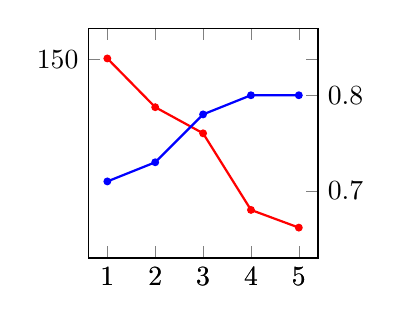
\begin{tikzpicture}

    \begin{axis}[
    width = 4.5cm,
    height= 4.5cm,
    enlarge x limits = 0.1,
    enlarge y limits = 0.1,
    legend columns=3,
    legend style={at={(0.05,-0.3)},anchor=west},
    xmax = 5,
    xtick={1,2,3,4,5},
    xmin = 1,
	ymin= 0,
	ymax=160,
	ytick={150,200},
	%ymode = log,
]
\addplot[thick, red, mark=*,
mark options={scale=0.5},
]
	plot coordinates {
		(1, 150.75)
		(2, 110.03)
		(3, 88.19)
		(4, 24.2)
		(5, 9.4)
	};
%\addlegendentry{search time}
\end{axis}

\begin{axis}[
    width = 4.5cm,
    height= 4.5cm,
	axis y line*=right,
    enlarge x limits = 0.1,
    enlarge y limits = 0.1,
    legend columns=3,
    legend style={at={(0.05,-0.3)},anchor=west},
    xmax = 5,
    xtick={1,2,3,4,5},
    xmin = 1,
	ymin=0.65,
	ymax=0.85,
]
\addplot[thick, blue, mark=*,
mark options={scale=0.5},
]
	plot coordinates {
		(1, 0.71)
		(2, 0.73)
		(3, 0.78)
		(4, 0.8)
		(5, 0.8)
	};
%\addlegendentry{coverage}
\end{axis}


\end{tikzpicture}

}
\end{minipage} &
\begin{minipage}{0.25\textwidth}
\resizebox{!}{3.0cm}{

    \begin{axis}[
    width = 5cm,
    height= 5cm,
    enlarge x limits = 0.1,
    enlarge y limits = 0.1,
    legend columns=3,
    legend style={at={(0.05,-0.3)},anchor=west},
    xmax = 5,
    xtick={1,2,3,4,5},
    xmin = 1,
	title = \#MUGS,
]
\addplot[thick, red, mark=*,
mark options={scale=0.5},
]
	plot coordinates {
		(1, 4.77)
		(2, 3.27)
		(3, 2.38)
		(4, 1.85)
		(5, 1.45)
	};
    \end{axis}

\end{tikzpicture}
\vspace{0.7cm}
\\

}
\end{minipage}
\end{tabular}
\vspace{-0.3cm}
\caption{\label{fig:ipc-local} Local explanation results on IPC 
benchmarks for SysS as a function of $|A|$. Left: coverage, \ie,
fraction of solved questions (dashed, right y-axis);
%
%OSP (dotted), \hlmcut (dashed dotted) (right y-axis)
%
and average runtime (solid, left y-axis). Right: average \#MUGS.}
%\joerg{integrate reference point coverage as horizontal lines into the left plot}
%\rebecca{update plot with new benchmark results with all ICP instances}
%
\vspace{-0.6cm}
\end{figure}


%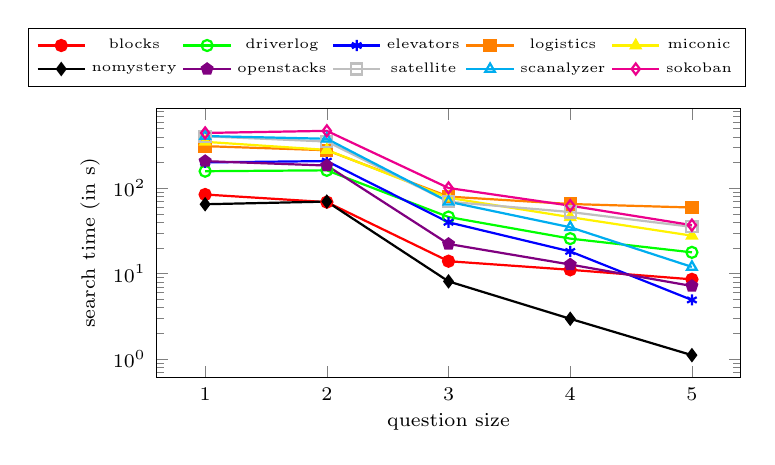
\begin{tikzpicture}[scale=1]
\tiny
    \begin{axis}[
    width = 9cm,
    height=5cm,
    enlarge x limits = 0.1,
    enlarge y limits = 0.1,
    ymode=log,
    xmin = 1,
	xmax = 5,
	xtick={1,2,3,4,5},
	xlabel = {question size},
	x label style = {font=\scriptsize},
	ylabel = {search time (in s)},
	legend style={at={(1.01,1.30)}},
	y label style = {font=\scriptsize},
	legend columns=5,
	x tick label style = {font=\scriptsize, yshift=-0.05cm},
	y tick label style = {font=\scriptsize, xshift=-0.05cm},
]
\addplot[thick, red, mark=*,
]
	plot coordinates {
		(1, 84.53)
		(2, 68.87)
		(3, 13.99)
		(4, 11.1)
		(5, 8.58)
	};
\addlegendentry{blocks}
\addplot[thick, green, mark=o,
]
	plot coordinates {
		(1, 158.49)
		(2, 162.32)
		(3, 46.09)
		(4, 25.74)
		(5, 17.77)
	};
\addlegendentry{driverlog}
\addplot[thick, blue, mark=asterisk,
]
	plot coordinates {
		(1, 201.02)
		(2, 208.31)
		(3, 39.96)
		(4, 18.21)
		(5, 4.92)
	};
\addlegendentry{elevators}
\addplot[thick, orange, mark=square*,
]
	plot coordinates {
		(1, 311.58)
		(2, 279.05)
		(3, 79.89)
		(4, 65.44)
		(5, 59.51)
	};
\addlegendentry{logistics}
\addplot[thick, yellow, mark=triangle*,
]
	plot coordinates {
		(1, 350.17)
		(2, 281.58)
		(3, 77.4)
		(4, 45.93)
		(5, 27.85)
	};
\addlegendentry{miconic}
\addplot[thick, black, mark=diamond*,
]
	plot coordinates {
		(1, 65.03)
		(2, 69.83)
		(3, 8.12)
		(4, 2.96)
		(5, 1.11)
	};
\addlegendentry{nomystery}
\addplot[thick, violet, mark=pentagon*,
]
	plot coordinates {
		(1, 208.06)
		(2, 184.65)
		(3, 22.27)
		(4, 12.79)
		(5, 7.17)
	};
\addlegendentry{openstacks}
\addplot[thick, lightgray, mark=square,
]
	plot coordinates {
		(1, 406.77)
		(2, 352.83)
		(3, 69.58)
		(4, 52.73)
		(5, 35.34)
	};
\addlegendentry{satellite}
\addplot[thick, cyan, mark=triangle,
]
	plot coordinates {
		(1, 409.17)
		(2, 380.07)
		(3, 69.56)
		(4, 34.95)
		(5, 12.0)
	};
\addlegendentry{scanalyzer}
\addplot[thick, magenta, mark=diamond,
]
	plot coordinates {
		(1, 444.74)
		(2, 470.68)
		(3, 100.78)
		(4, 62.61)
		(5, 37.0)
	};
\addlegendentry{sokoban}

    \end{axis}

\end{tikzpicture}
\\

%
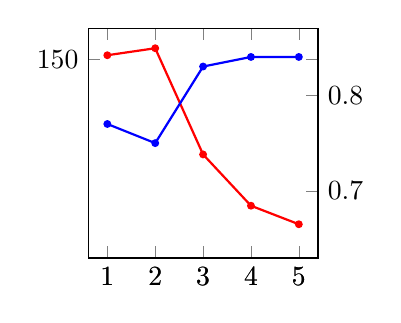
\begin{tikzpicture}

    \begin{axis}[
    width = 4.5cm,
    height= 4.5cm,
    enlarge x limits = 0.1,
    enlarge y limits = 0.1,
    legend columns=3,
    legend style={at={(0.05,-0.2)},anchor=west},
    xmin = 1,
    xmax = 5,
    xtick={1,2,3,4,5},
	ymin= 120,
	ymax=220,
	ymin= 0,
	ymax=160,
	ytick={150,200},
	%ymode = log,
]
	\addplot[thick, red, mark=*, mark options={scale=0.5}]
		plot coordinates {
			(1, 153.43)
			(2, 159.28)
			(3, 70.55)
			(4, 27.7)
			(5, 12.22)
		};
%\addlegendentry{search time}

\end{axis}

\begin{axis}[
    width = 4.5cm,
    height= 4.5cm,
	axis y line*=right,
    enlarge x limits = 0.1,
    enlarge y limits = 0.1,
    legend columns=3,
    legend style={at={(0.5,-0.2)},anchor=west},
    xmax = 5,
    xtick={1,2,3,4,5},
    xmin = 1,
	ymin=0.65,
	ymax=0.85,
]
	\addplot[thick, blue, mark=*, mark options={scale=0.5}]
		plot coordinates {
			(1, 0.77)
			(2, 0.75)
			(3, 0.83)
			(4, 0.84)
			(5, 0.84)
		};
%\addlegendentry{coverage}
\end{axis}

\end{tikzpicture}


The results are very consistent across domains, and are much stronger
still in some cases. Of the 42 domains that have at least one instance
with $\geq 6$ goals, 6 domains have much stronger ($> 20\%$) increases
in coverage from $|A|=1$ to $|A|=5$,
%There are 37 domains wich have at least one problems with more than 5 goals.
%
%% For coverage, Blocksworld, Depots, Elevators, NoMystery, Openstacks, Visiteal
%
and in 15 domains average runtime decreases by at least one order of
magnitude. 
%
%% runtime: 
%%1 order blocks, drive, floortile, elevators, grip,
%% mic, log, nomystrey, pathway, sat, soko, stor, tetr, tpp,
%% transp, wood; 
%% 2 orders depots, scan, trucks
%
The average number of MUGS for $|A|=5$ is less than $5$ in all
domains, including ones like Floortile, Gripper, Miconic, Woodworking
where global explanations can be large as shown in
Figure~\ref{table:coverage_ipc}.





%%%%%%%%%%%%%%%%%%%%%%%%%%%%%%%%%%%%%%%%%%%%%%%%%%%%%%%%%%%%%%%%%%%%
%%%%%%%%%%%%%%%%%%%%%%%%%%%%%%%%%%%%%%%%%%%%%%%%%%%%%%%%%%%%%%%%%%%%
%%%%%%%%%%%%%%%%%%%%%%%%%%%%%%%%%%%%%%%%%%%%%%%%%%%%%%%%%%%%%%%%%%%%
%%%% Action-Set Properties, SUBMISSION VERSION

\subsection{Action-Set Properties}

To evaluate the use of our framework with more complex plan
properties, we experimented with the compilation of action-set
properties as per Section~\ref{actionsetprops}. 
%
We extended four domains with action-set properties: NoMystery,
Rovers, and TPP as per \cite{nakhost:etal:icaps-12}, with controlled
resource constrainedness (\cf\ Section~\ref{background}); plus the
Blocksworld as an intuitively differently structured domain.
%
In NoMystery, the action-set properties are as in our illustrative
example. In Rovers, the properties ask which rover or camera is used
for which observation. In TPP, they ask which road segments are used,
and which goods are bought at which markets. In Blocksworld, we
include two hands and the properties ask which hand is used for which
blocks.
%
We set the original goal facts as hard goals, so that the analysis
determines exclusion relations over conjunctions of action-set
properties.

We encoded resource consumption into the FDR state variables, enabling
the use of trap learning which turns out to be highly beneficial
here. We generated benchmarks of sizes around the feasibility
borderline, and we experimented with resource constrainedness
$x \in \{1.0, 1.25, 1.5, 2.0\}$. For reference, we ran \astar\
with \hlmcut\ as before, on all goal facts (original plus compiled
action-set properties). Current OSP planners cannot handle hard goals,
so we used our base planner with trap learning instead as a second
reference point.

%% \joerg{presumably, include a figure with one plot per domain,
%% fixing number of goals as in IJCAI long versions (main paper plot),
%% and with fixed constrainedness factor x. use same x for both global
%% and local explanations. x=2.0 is too high, Blocks and TPP
%% apparently typically all goals achievable easil for base
%% planner. x=1.0 shows off advantage of trap learning, but does not
%% challenge the reference points enough. for x=1.5 on the other hand
%% trap learning is way less important than for 1.0. Try x=1.25 and
%% see what it looks like.}
%
\begin{figure}[h!]
\vspace{-0.2cm}
\small
\centering

\tiny
\centering
\begin{tikzpicture}
    \begin{axis}[
    width = 5cm,
    height=4cm,
    enlarge x limits = 0.1,
    enlarge y limits = 0.07,
    legend columns=1,
    ybar,
    bar width=1pt,
    ymin = 0,
    ymax = 10,
	compat=1.6,
	title={},
	xticklabels={,,},
	xtick style={draw=none},
	%ylabel=goals 06,
	at={(0,0)},
]
\addplot+[ybar, bar shift =-4.0pt, red,
]
plot coordinates {
(07, 2) %c_125
(08, 0) %c_125
(03, 10) %c_125
(10, 0) %c_125
(06, 3) %c_125
(09, 0) %c_125
(02, 10) %c_125
(05, 5) %c_125
(04, 7) %c_125
(01, 10) %c_125
};
\label{plot:props_hff_bu_53}
\addplot+[ybar, bar shift =-2.0pt, blue,
]
plot coordinates {
(07, 3) %c_125
(08, 1) %c_125
(03, 10) %c_125
(10, 0) %c_125
(06, 6) %c_125
(09, 4) %c_125
(02, 10) %c_125
(05, 10) %c_125
(04, 10) %c_125
(01, 10) %c_125
};
\label{plot:props_hff_td_53}
\addplot+[ybar, bar shift =0.0pt, green,
]
plot coordinates {
(07, 0) %c_125
(08, 0) %c_125
(03, 6) %c_125
(10, 0) %c_125
(06, 1) %c_125
(09, 0) %c_125
(02, 8) %c_125
(05, 4) %c_125
(04, 4) %c_125
(01, 9) %c_125
};
\label{plot:props_trap_bu_53}
\addplot+[ybar, bar shift =2.0pt, orange,
]
plot coordinates {
(07, 0) %c_125
(08, 0) %c_125
(03, 6) %c_125
(10, 0) %c_125
(06, 2) %c_125
(09, 0) %c_125
(02, 9) %c_125
(05, 4) %c_125
(04, 4) %c_125
(01, 9) %c_125
};
\label{plot:props_trap_td_53}

%lmcut
\addplot+[only marks, mark = -, mark options = {thick, red, dashed}, mark size = 0.15cm, black,
]
plot coordinates {
(02, 10)
(01, 10)
(04, 10)
(03, 10)
(07, 10)
(08, 10)
(06, 10)
(10, 10)
(05, 10)
(09, 10)
};

%trap first meta node top down
\addplot+[only marks, mark = -, mark options = {thick, black}, mark size = 0.15cm, black,
]
plot coordinates {
(01, 9)
(02, 9)
(03, 6)
(04, 4)
(05, 4)
(06, 2)
(07, 0)
(08, 0)
(09, 0)
(10, 2)
};
    \end{axis}
    \hfill
    
%\node[draw, align=center] (test) at (2,-2) {
%\ref{plot:props_hff_bu_53} props-hff-bu\\
%\ref{plot:props_hff_td_53} props-hff-td\\
%\ref{plot:props_trap_bu_53} props-trap-bu\\
%\ref{plot:props_trap_td_53} props-trap-td\\
%};




    \begin{axis}[
    width = 5cm,
    height=4cm,
    enlarge x limits = 0.1,
    enlarge y limits = 0.1,
    legend columns=1,
    ybar,
    bar width=1pt,
    ymin = 0,
    ymax = 10,
	compat=1.6,
	title=NoMystery,
	title style={yshift=-1.5ex},
	%ylabel=goals 6,
	%xticklabels={,,},
	%xtick style={draw=none},
	xtick= {1,5,10},
	at={(4cm,0)},
]
\addplot+[ybar, bar shift =-4.0pt, red,
]
plot coordinates {
(04, 8) %c_100
(09, 2) %c_100
(10, 2) %c_100
(08, 4) %c_100
(02, 9) %c_100
(07, 5) %c_100
(06, 5) %c_100
(05, 5) %c_100
(03, 8) %c_100
(01, 10) %c_100
};
\label{plot:props_bu_hff_46}
\addplot+[ybar, bar shift =-2.0pt, blue,
]
plot coordinates {
(04, 8) %c_100
(09, 2) %c_100
(10, 1) %c_100
(08, 2) %c_100
(02, 9) %c_100
(07, 2) %c_100
(06, 2) %c_100
(05, 5) %c_100
(03, 8) %c_100
(01, 10) %c_100
};
\label{plot:props_td_hff_46}
\addplot+[ybar, bar shift =0.0pt, green,
]
plot coordinates {
(04, 9) %c_100
(09, 8) %c_100
(10, 8) %c_100
(08, 8) %c_100
(02, 10) %c_100
(07, 8) %c_100
(06, 9) %c_100
(05, 9) %c_100
(03, 10) %c_100
(01, 10) %c_100
};
\label{plot:props_bu_trap_46}
\addplot+[ybar, bar shift =2.0pt, orange,
]
plot coordinates {
(04, 8) %c_100
(09, 8) %c_100
(03, 8) %c_100
(08, 8) %c_100
(02, 10) %c_100
(07, 8) %c_100
(06, 7) %c_100
(05, 7) %c_100
(10, 7) %c_100
(01, 10) %c_100
};
\label{plot:props_td_trap_46}

%lmcut
\addplot+[only marks, mark = -, mark options = {thick, red, dashed}, mark size = 0.15cm, black,
]
plot coordinates {
(01, 10)
(02, 10)
(03, 10)
(04, 10)
(05, 10)
(06, 10)
(07, 10)
(08, 10)
(09, 10)
(10, 10)
};

%trap first meta node top down
\addplot+[only marks, mark = -, mark options = {thick, black}, mark size = 0.15cm, black,
]
plot coordinates {
(01, 10)
(02, 10)
(03, 10)
(04, 10)
(05, 10)
(06, 10)
(07, 10)
(08, 10)
(09, 10)
(10, 10)
};
    \end{axis}
    \hfill
    
%\node[draw, align=center] (test) at (8,-18) {
%\ref{plot:props_bu_hff_46} props-bu-hff\\
%\ref{plot:props_td_hff_46} props-td-hff\\
%\ref{plot:props_bu_trap_46} props-bu-trap\\
%\ref{plot:props_td_trap_46} props-td-trap\\
%};




%\begin{axis}[
width = 5cm,
height=4cm,
enlarge x limits = 0.1,
enlarge y limits = 0.1,
legend columns=1,
ybar,
bar width=1pt,
ymin = 0,
ymax = 10,
compat=1.6,
at={(0,-2.5cm)},
	xticklabels={,,},
	xtick style={draw=none},
]
\addplot+[ybar, bar shift =-2.5pt, red,
]
plot coordinates {
(08, 4)
(09, 3)
(01, 10)
(03, 8)
(02, 10)
(04, 9)
(05, 10)
(06, 6)
(10, 2)
(07, 6)
};
\label{plot:properties_hff_bu_52}
\addplot+[ybar, bar shift =-1.0pt, blue,
]
plot coordinates {
(01, 10)
(08, 5)
(02, 10)
(04, 9)
(03, 8)
(05, 10)
(06, 5)
(10, 5)
(07, 7)
(09, 6)
};
\label{plot:properties_hff_td_52}
\addplot+[ybar, bar shift =1.0pt, green,
]
plot coordinates {
(09, 10)
(01, 10)
(02, 10)
(04, 10)
(03, 10)
(05, 10)
(06, 10)
(10, 10)
(07, 10)
(08, 10)
};
\label{plot:properties_trap_prefop_bu_52}
\addplot+[ybar, bar shift =2.5pt, orange,
]
plot coordinates {
(01, 10)
(08, 10)
(02, 10)
(03, 10)
(04, 10)
(05, 10)
(06, 10)
(10, 10)
(07, 10)
(09, 10)
};
\label{plot:properties_trap_prefop_td_52}

%start node sysW
\addplot+[only marks, mark = -, mark options = {thick}, mark size = 0.2cm, black,
]
plot coordinates {
(02, 10)
(01, 10)
(04, 10)
(03, 10)
(07, 10)
(08, 10)
(06, 10)
(10, 10)
(05, 10)
(09, 10)
};
%optimal
\addplot+[only marks, mark = -, mark options = {thick, red, dashed}, mark size = 0.2cm, black,
]
plot coordinates {
(03, 7)
(05, 6)
(07, 0)
(09, 3)
(01, 9)
(02, 8)
(04, 7)
(06, 2)
(08, 3)
(10, 2)
};

\end{axis}



    \begin{axis}[
    width = 5cm,
    height=4cm,
    enlarge x limits = 0.1,
    enlarge y limits = 0.1,
    legend columns=1,
    ybar,
    bar width=1pt,
    ymin = 0,
    ymax = 10,
compat=1.6,
%title=c 150,
%ylabel=goals 7,
at={(4cm,-2.5cm)},
]
\addplot+[ybar, bar shift =-4.0pt, red,
]
plot coordinates {
(07, 4) %c_150
(06, 5) %c_150
(05, 6) %c_150
(09, 3) %c_150
(08, 3) %c_150
(10, 2) %c_150
(01, 10) %c_150
(04, 8) %c_150
(03, 10) %c_150
(02, 10) %c_150
};
\label{plot:props_bu_hff_49}
\addplot+[ybar, bar shift =-2.0pt, blue,
]
plot coordinates {
(07, 5) %c_150
(06, 6) %c_150
(05, 7) %c_150
(09, 4) %c_150
(08, 4) %c_150
(10, 3) %c_150
(01, 10) %c_150
(04, 8) %c_150
(03, 10) %c_150
(02, 10) %c_150
};
\label{plot:props_td_hff_49}
\addplot+[ybar, bar shift =0.0pt, green,
]
plot coordinates {
(07, 4) %c_150
(06, 5) %c_150
(05, 8) %c_150
(09, 3) %c_150
(08, 3) %c_150
(03, 10) %c_150
(01, 10) %c_150
(04, 9) %c_150
(10, 2) %c_150
(02, 10) %c_150
};
\label{plot:props_bu_trap_49}
\addplot+[ybar, bar shift =2.0pt, orange,
]
plot coordinates {
(07, 8) %c_150
(06, 9) %c_150
(05, 9) %c_150
(09, 5) %c_150
(08, 6) %c_150
(10, 3) %c_150
(01, 10) %c_150
(04, 10) %c_150
(03, 10) %c_150
(02, 10) %c_150
};
\label{plot:props_td_trap_49}

%lmcut
\addplot+[only marks, mark = -, mark options = {thick, red, dashed}, mark size = 0.15cm, black,
]
plot coordinates {
(02, 10)
(01, 10)
(04, 10)
(03, 10)
(07, 10)
(08, 10)
(06, 10)
(10, 10)
(05, 10)
(09, 10)
};

%trap first meta node top down
\addplot+[only marks, mark = -, mark options = {thick, black}, mark size = 0.15cm, black,
]
plot coordinates {
(01, 10)
(02, 10)
(03, 10)
(04, 10)
(05, 9)
(06, 9)
(07, 10)
(08, 10)
(09, 10)
(10, 9)
};
    \end{axis}
    \hfill
    
%\node[draw, align=center] (test) at (8,-18) {
%\ref{plot:props_bu_hff_49} props-bu-hff\\
%\ref{plot:props_td_hff_49} props-td-hff\\
%\ref{plot:props_bu_trap_49} props-bu-trap\\
%\ref{plot:props_td_trap_49} props-td-trap\\
%};




\node[draw] (test) at (3.5,-3.0) {
\ref{plot:props_bu_hff_94}   SysS
\ref{plot:props_td_hff_94}   SysW
\ref{plot:props_bu_trap_94} SysS trap 
\ref{plot:props_td_trap_94} SysW trap 
%\ref{plot:baseline_lmcut} \hlmcut
%\ref{plot:baseline_sysW_node} trap
};
\end{tikzpicture}


\tiny
\centering
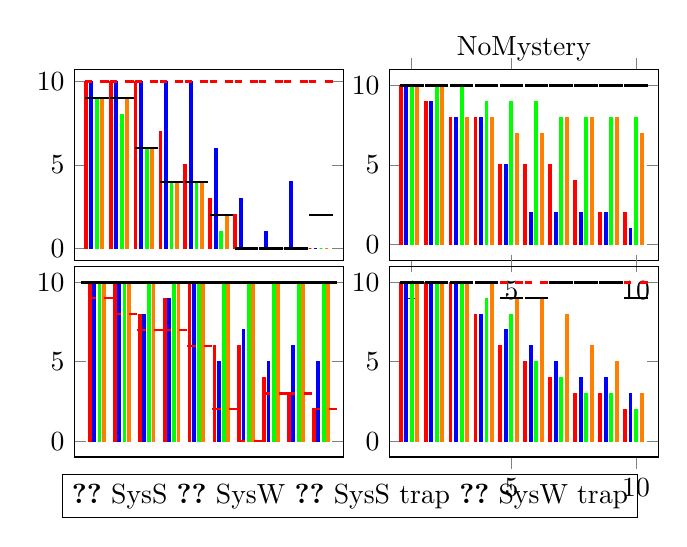
\begin{tikzpicture}
    \begin{axis}[
    width = 5cm,
    height=4cm,
    enlarge x limits = 0.1,
    enlarge y limits = 0.07,
    legend columns=1,
    ybar,
    bar width=1pt,
    ymin = 0,
    ymax = 10,
	compat=1.6,
	title={},
	xticklabels={,,},
	xtick style={draw=none},
	%ylabel=goals 06,
	at={(0,0)},
]
\addplot+[ybar, bar shift =-4.0pt, red,
]
plot coordinates {
(07, 2) %c_125
(08, 0) %c_125
(03, 10) %c_125
(10, 0) %c_125
(06, 3) %c_125
(09, 0) %c_125
(02, 10) %c_125
(05, 5) %c_125
(04, 7) %c_125
(01, 10) %c_125
};
\label{plot:props_hff_bu_53}
\addplot+[ybar, bar shift =-2.0pt, blue,
]
plot coordinates {
(07, 3) %c_125
(08, 1) %c_125
(03, 10) %c_125
(10, 0) %c_125
(06, 6) %c_125
(09, 4) %c_125
(02, 10) %c_125
(05, 10) %c_125
(04, 10) %c_125
(01, 10) %c_125
};
\label{plot:props_hff_td_53}
\addplot+[ybar, bar shift =0.0pt, green,
]
plot coordinates {
(07, 0) %c_125
(08, 0) %c_125
(03, 6) %c_125
(10, 0) %c_125
(06, 1) %c_125
(09, 0) %c_125
(02, 8) %c_125
(05, 4) %c_125
(04, 4) %c_125
(01, 9) %c_125
};
\label{plot:props_trap_bu_53}
\addplot+[ybar, bar shift =2.0pt, orange,
]
plot coordinates {
(07, 0) %c_125
(08, 0) %c_125
(03, 6) %c_125
(10, 0) %c_125
(06, 2) %c_125
(09, 0) %c_125
(02, 9) %c_125
(05, 4) %c_125
(04, 4) %c_125
(01, 9) %c_125
};
\label{plot:props_trap_td_53}

%lmcut
\addplot+[only marks, mark = -, mark options = {thick, red, dashed}, mark size = 0.15cm, black,
]
plot coordinates {
(02, 10)
(01, 10)
(04, 10)
(03, 10)
(07, 10)
(08, 10)
(06, 10)
(10, 10)
(05, 10)
(09, 10)
};

%trap first meta node top down
\addplot+[only marks, mark = -, mark options = {thick, black}, mark size = 0.15cm, black,
]
plot coordinates {
(01, 9)
(02, 9)
(03, 6)
(04, 4)
(05, 4)
(06, 2)
(07, 0)
(08, 0)
(09, 0)
(10, 2)
};
    \end{axis}
    \hfill
    
%\node[draw, align=center] (test) at (2,-2) {
%\ref{plot:props_hff_bu_53} props-hff-bu\\
%\ref{plot:props_hff_td_53} props-hff-td\\
%\ref{plot:props_trap_bu_53} props-trap-bu\\
%\ref{plot:props_trap_td_53} props-trap-td\\
%};




    \begin{axis}[
    width = 5cm,
    height=4cm,
    enlarge x limits = 0.1,
    enlarge y limits = 0.1,
    legend columns=1,
    ybar,
    bar width=1pt,
    ymin = 0,
    ymax = 10,
	compat=1.6,
	title=NoMystery,
	title style={yshift=-1.5ex},
	%ylabel=goals 6,
	%xticklabels={,,},
	%xtick style={draw=none},
	xtick= {1,5,10},
	at={(4cm,0)},
]
\addplot+[ybar, bar shift =-4.0pt, red,
]
plot coordinates {
(04, 8) %c_100
(09, 2) %c_100
(10, 2) %c_100
(08, 4) %c_100
(02, 9) %c_100
(07, 5) %c_100
(06, 5) %c_100
(05, 5) %c_100
(03, 8) %c_100
(01, 10) %c_100
};
\label{plot:props_bu_hff_46}
\addplot+[ybar, bar shift =-2.0pt, blue,
]
plot coordinates {
(04, 8) %c_100
(09, 2) %c_100
(10, 1) %c_100
(08, 2) %c_100
(02, 9) %c_100
(07, 2) %c_100
(06, 2) %c_100
(05, 5) %c_100
(03, 8) %c_100
(01, 10) %c_100
};
\label{plot:props_td_hff_46}
\addplot+[ybar, bar shift =0.0pt, green,
]
plot coordinates {
(04, 9) %c_100
(09, 8) %c_100
(10, 8) %c_100
(08, 8) %c_100
(02, 10) %c_100
(07, 8) %c_100
(06, 9) %c_100
(05, 9) %c_100
(03, 10) %c_100
(01, 10) %c_100
};
\label{plot:props_bu_trap_46}
\addplot+[ybar, bar shift =2.0pt, orange,
]
plot coordinates {
(04, 8) %c_100
(09, 8) %c_100
(03, 8) %c_100
(08, 8) %c_100
(02, 10) %c_100
(07, 8) %c_100
(06, 7) %c_100
(05, 7) %c_100
(10, 7) %c_100
(01, 10) %c_100
};
\label{plot:props_td_trap_46}

%lmcut
\addplot+[only marks, mark = -, mark options = {thick, red, dashed}, mark size = 0.15cm, black,
]
plot coordinates {
(01, 10)
(02, 10)
(03, 10)
(04, 10)
(05, 10)
(06, 10)
(07, 10)
(08, 10)
(09, 10)
(10, 10)
};

%trap first meta node top down
\addplot+[only marks, mark = -, mark options = {thick, black}, mark size = 0.15cm, black,
]
plot coordinates {
(01, 10)
(02, 10)
(03, 10)
(04, 10)
(05, 10)
(06, 10)
(07, 10)
(08, 10)
(09, 10)
(10, 10)
};
    \end{axis}
    \hfill
    
%\node[draw, align=center] (test) at (8,-18) {
%\ref{plot:props_bu_hff_46} props-bu-hff\\
%\ref{plot:props_td_hff_46} props-td-hff\\
%\ref{plot:props_bu_trap_46} props-bu-trap\\
%\ref{plot:props_td_trap_46} props-td-trap\\
%};




\begin{axis}[
width = 5cm,
height=4cm,
enlarge x limits = 0.1,
enlarge y limits = 0.1,
legend columns=1,
ybar,
bar width=1pt,
ymin = 0,
ymax = 10,
compat=1.6,
at={(0,-2.5cm)},
	xticklabels={,,},
	xtick style={draw=none},
]
\addplot+[ybar, bar shift =-2.5pt, red,
]
plot coordinates {
(08, 4)
(09, 3)
(01, 10)
(03, 8)
(02, 10)
(04, 9)
(05, 10)
(06, 6)
(10, 2)
(07, 6)
};
\label{plot:properties_hff_bu_52}
\addplot+[ybar, bar shift =-1.0pt, blue,
]
plot coordinates {
(01, 10)
(08, 5)
(02, 10)
(04, 9)
(03, 8)
(05, 10)
(06, 5)
(10, 5)
(07, 7)
(09, 6)
};
\label{plot:properties_hff_td_52}
\addplot+[ybar, bar shift =1.0pt, green,
]
plot coordinates {
(09, 10)
(01, 10)
(02, 10)
(04, 10)
(03, 10)
(05, 10)
(06, 10)
(10, 10)
(07, 10)
(08, 10)
};
\label{plot:properties_trap_prefop_bu_52}
\addplot+[ybar, bar shift =2.5pt, orange,
]
plot coordinates {
(01, 10)
(08, 10)
(02, 10)
(03, 10)
(04, 10)
(05, 10)
(06, 10)
(10, 10)
(07, 10)
(09, 10)
};
\label{plot:properties_trap_prefop_td_52}

%start node sysW
\addplot+[only marks, mark = -, mark options = {thick}, mark size = 0.2cm, black,
]
plot coordinates {
(02, 10)
(01, 10)
(04, 10)
(03, 10)
(07, 10)
(08, 10)
(06, 10)
(10, 10)
(05, 10)
(09, 10)
};
%optimal
\addplot+[only marks, mark = -, mark options = {thick, red, dashed}, mark size = 0.2cm, black,
]
plot coordinates {
(03, 7)
(05, 6)
(07, 0)
(09, 3)
(01, 9)
(02, 8)
(04, 7)
(06, 2)
(08, 3)
(10, 2)
};

\end{axis}



    \begin{axis}[
    width = 5cm,
    height=4cm,
    enlarge x limits = 0.1,
    enlarge y limits = 0.1,
    legend columns=1,
    ybar,
    bar width=1pt,
    ymin = 0,
    ymax = 10,
compat=1.6,
%title=c 150,
%ylabel=goals 7,
at={(4cm,-2.5cm)},
]
\addplot+[ybar, bar shift =-4.0pt, red,
]
plot coordinates {
(07, 4) %c_150
(06, 5) %c_150
(05, 6) %c_150
(09, 3) %c_150
(08, 3) %c_150
(10, 2) %c_150
(01, 10) %c_150
(04, 8) %c_150
(03, 10) %c_150
(02, 10) %c_150
};
\label{plot:props_bu_hff_49}
\addplot+[ybar, bar shift =-2.0pt, blue,
]
plot coordinates {
(07, 5) %c_150
(06, 6) %c_150
(05, 7) %c_150
(09, 4) %c_150
(08, 4) %c_150
(10, 3) %c_150
(01, 10) %c_150
(04, 8) %c_150
(03, 10) %c_150
(02, 10) %c_150
};
\label{plot:props_td_hff_49}
\addplot+[ybar, bar shift =0.0pt, green,
]
plot coordinates {
(07, 4) %c_150
(06, 5) %c_150
(05, 8) %c_150
(09, 3) %c_150
(08, 3) %c_150
(03, 10) %c_150
(01, 10) %c_150
(04, 9) %c_150
(10, 2) %c_150
(02, 10) %c_150
};
\label{plot:props_bu_trap_49}
\addplot+[ybar, bar shift =2.0pt, orange,
]
plot coordinates {
(07, 8) %c_150
(06, 9) %c_150
(05, 9) %c_150
(09, 5) %c_150
(08, 6) %c_150
(10, 3) %c_150
(01, 10) %c_150
(04, 10) %c_150
(03, 10) %c_150
(02, 10) %c_150
};
\label{plot:props_td_trap_49}

%lmcut
\addplot+[only marks, mark = -, mark options = {thick, red, dashed}, mark size = 0.15cm, black,
]
plot coordinates {
(02, 10)
(01, 10)
(04, 10)
(03, 10)
(07, 10)
(08, 10)
(06, 10)
(10, 10)
(05, 10)
(09, 10)
};

%trap first meta node top down
\addplot+[only marks, mark = -, mark options = {thick, black}, mark size = 0.15cm, black,
]
plot coordinates {
(01, 10)
(02, 10)
(03, 10)
(04, 10)
(05, 9)
(06, 9)
(07, 10)
(08, 10)
(09, 10)
(10, 9)
};
    \end{axis}
    \hfill
    
%\node[draw, align=center] (test) at (8,-18) {
%\ref{plot:props_bu_hff_49} props-bu-hff\\
%\ref{plot:props_td_hff_49} props-td-hff\\
%\ref{plot:props_bu_trap_49} props-bu-trap\\
%\ref{plot:props_td_trap_49} props-td-trap\\
%};




\node[draw] (test) at (3.5,-3.0) {
\ref{plot:props_bu_hff_94}   SysS
\ref{plot:props_td_hff_94}   SysW
\ref{plot:props_bu_trap_94} SysS trap 
\ref{plot:props_td_trap_94} SysW trap 
%\ref{plot:baseline_lmcut} \hlmcut
%\ref{plot:baseline_sysW_node} trap
};
\end{tikzpicture}

\tiny
\centering
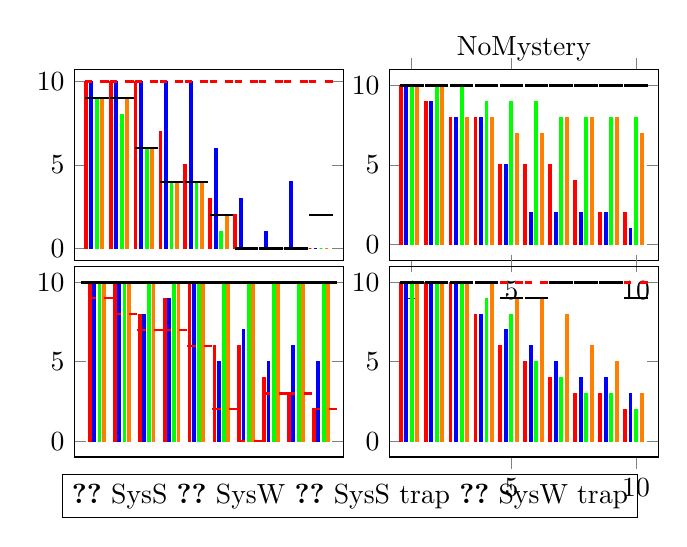
\begin{tikzpicture}
    \begin{axis}[
    width = 5cm,
    height=4cm,
    enlarge x limits = 0.1,
    enlarge y limits = 0.07,
    legend columns=1,
    ybar,
    bar width=1pt,
    ymin = 0,
    ymax = 10,
	compat=1.6,
	title={},
	xticklabels={,,},
	xtick style={draw=none},
	%ylabel=goals 06,
	at={(0,0)},
]
\addplot+[ybar, bar shift =-4.0pt, red,
]
plot coordinates {
(07, 2) %c_125
(08, 0) %c_125
(03, 10) %c_125
(10, 0) %c_125
(06, 3) %c_125
(09, 0) %c_125
(02, 10) %c_125
(05, 5) %c_125
(04, 7) %c_125
(01, 10) %c_125
};
\label{plot:props_hff_bu_53}
\addplot+[ybar, bar shift =-2.0pt, blue,
]
plot coordinates {
(07, 3) %c_125
(08, 1) %c_125
(03, 10) %c_125
(10, 0) %c_125
(06, 6) %c_125
(09, 4) %c_125
(02, 10) %c_125
(05, 10) %c_125
(04, 10) %c_125
(01, 10) %c_125
};
\label{plot:props_hff_td_53}
\addplot+[ybar, bar shift =0.0pt, green,
]
plot coordinates {
(07, 0) %c_125
(08, 0) %c_125
(03, 6) %c_125
(10, 0) %c_125
(06, 1) %c_125
(09, 0) %c_125
(02, 8) %c_125
(05, 4) %c_125
(04, 4) %c_125
(01, 9) %c_125
};
\label{plot:props_trap_bu_53}
\addplot+[ybar, bar shift =2.0pt, orange,
]
plot coordinates {
(07, 0) %c_125
(08, 0) %c_125
(03, 6) %c_125
(10, 0) %c_125
(06, 2) %c_125
(09, 0) %c_125
(02, 9) %c_125
(05, 4) %c_125
(04, 4) %c_125
(01, 9) %c_125
};
\label{plot:props_trap_td_53}

%lmcut
\addplot+[only marks, mark = -, mark options = {thick, red, dashed}, mark size = 0.15cm, black,
]
plot coordinates {
(02, 10)
(01, 10)
(04, 10)
(03, 10)
(07, 10)
(08, 10)
(06, 10)
(10, 10)
(05, 10)
(09, 10)
};

%trap first meta node top down
\addplot+[only marks, mark = -, mark options = {thick, black}, mark size = 0.15cm, black,
]
plot coordinates {
(01, 9)
(02, 9)
(03, 6)
(04, 4)
(05, 4)
(06, 2)
(07, 0)
(08, 0)
(09, 0)
(10, 2)
};
    \end{axis}
    \hfill
    
%\node[draw, align=center] (test) at (2,-2) {
%\ref{plot:props_hff_bu_53} props-hff-bu\\
%\ref{plot:props_hff_td_53} props-hff-td\\
%\ref{plot:props_trap_bu_53} props-trap-bu\\
%\ref{plot:props_trap_td_53} props-trap-td\\
%};




    \begin{axis}[
    width = 5cm,
    height=4cm,
    enlarge x limits = 0.1,
    enlarge y limits = 0.1,
    legend columns=1,
    ybar,
    bar width=1pt,
    ymin = 0,
    ymax = 10,
	compat=1.6,
	title=NoMystery,
	title style={yshift=-1.5ex},
	%ylabel=goals 6,
	%xticklabels={,,},
	%xtick style={draw=none},
	xtick= {1,5,10},
	at={(4cm,0)},
]
\addplot+[ybar, bar shift =-4.0pt, red,
]
plot coordinates {
(04, 8) %c_100
(09, 2) %c_100
(10, 2) %c_100
(08, 4) %c_100
(02, 9) %c_100
(07, 5) %c_100
(06, 5) %c_100
(05, 5) %c_100
(03, 8) %c_100
(01, 10) %c_100
};
\label{plot:props_bu_hff_46}
\addplot+[ybar, bar shift =-2.0pt, blue,
]
plot coordinates {
(04, 8) %c_100
(09, 2) %c_100
(10, 1) %c_100
(08, 2) %c_100
(02, 9) %c_100
(07, 2) %c_100
(06, 2) %c_100
(05, 5) %c_100
(03, 8) %c_100
(01, 10) %c_100
};
\label{plot:props_td_hff_46}
\addplot+[ybar, bar shift =0.0pt, green,
]
plot coordinates {
(04, 9) %c_100
(09, 8) %c_100
(10, 8) %c_100
(08, 8) %c_100
(02, 10) %c_100
(07, 8) %c_100
(06, 9) %c_100
(05, 9) %c_100
(03, 10) %c_100
(01, 10) %c_100
};
\label{plot:props_bu_trap_46}
\addplot+[ybar, bar shift =2.0pt, orange,
]
plot coordinates {
(04, 8) %c_100
(09, 8) %c_100
(03, 8) %c_100
(08, 8) %c_100
(02, 10) %c_100
(07, 8) %c_100
(06, 7) %c_100
(05, 7) %c_100
(10, 7) %c_100
(01, 10) %c_100
};
\label{plot:props_td_trap_46}

%lmcut
\addplot+[only marks, mark = -, mark options = {thick, red, dashed}, mark size = 0.15cm, black,
]
plot coordinates {
(01, 10)
(02, 10)
(03, 10)
(04, 10)
(05, 10)
(06, 10)
(07, 10)
(08, 10)
(09, 10)
(10, 10)
};

%trap first meta node top down
\addplot+[only marks, mark = -, mark options = {thick, black}, mark size = 0.15cm, black,
]
plot coordinates {
(01, 10)
(02, 10)
(03, 10)
(04, 10)
(05, 10)
(06, 10)
(07, 10)
(08, 10)
(09, 10)
(10, 10)
};
    \end{axis}
    \hfill
    
%\node[draw, align=center] (test) at (8,-18) {
%\ref{plot:props_bu_hff_46} props-bu-hff\\
%\ref{plot:props_td_hff_46} props-td-hff\\
%\ref{plot:props_bu_trap_46} props-bu-trap\\
%\ref{plot:props_td_trap_46} props-td-trap\\
%};




\begin{axis}[
width = 5cm,
height=4cm,
enlarge x limits = 0.1,
enlarge y limits = 0.1,
legend columns=1,
ybar,
bar width=1pt,
ymin = 0,
ymax = 10,
compat=1.6,
at={(0,-2.5cm)},
	xticklabels={,,},
	xtick style={draw=none},
]
\addplot+[ybar, bar shift =-2.5pt, red,
]
plot coordinates {
(08, 4)
(09, 3)
(01, 10)
(03, 8)
(02, 10)
(04, 9)
(05, 10)
(06, 6)
(10, 2)
(07, 6)
};
\label{plot:properties_hff_bu_52}
\addplot+[ybar, bar shift =-1.0pt, blue,
]
plot coordinates {
(01, 10)
(08, 5)
(02, 10)
(04, 9)
(03, 8)
(05, 10)
(06, 5)
(10, 5)
(07, 7)
(09, 6)
};
\label{plot:properties_hff_td_52}
\addplot+[ybar, bar shift =1.0pt, green,
]
plot coordinates {
(09, 10)
(01, 10)
(02, 10)
(04, 10)
(03, 10)
(05, 10)
(06, 10)
(10, 10)
(07, 10)
(08, 10)
};
\label{plot:properties_trap_prefop_bu_52}
\addplot+[ybar, bar shift =2.5pt, orange,
]
plot coordinates {
(01, 10)
(08, 10)
(02, 10)
(03, 10)
(04, 10)
(05, 10)
(06, 10)
(10, 10)
(07, 10)
(09, 10)
};
\label{plot:properties_trap_prefop_td_52}

%start node sysW
\addplot+[only marks, mark = -, mark options = {thick}, mark size = 0.2cm, black,
]
plot coordinates {
(02, 10)
(01, 10)
(04, 10)
(03, 10)
(07, 10)
(08, 10)
(06, 10)
(10, 10)
(05, 10)
(09, 10)
};
%optimal
\addplot+[only marks, mark = -, mark options = {thick, red, dashed}, mark size = 0.2cm, black,
]
plot coordinates {
(03, 7)
(05, 6)
(07, 0)
(09, 3)
(01, 9)
(02, 8)
(04, 7)
(06, 2)
(08, 3)
(10, 2)
};

\end{axis}



    \begin{axis}[
    width = 5cm,
    height=4cm,
    enlarge x limits = 0.1,
    enlarge y limits = 0.1,
    legend columns=1,
    ybar,
    bar width=1pt,
    ymin = 0,
    ymax = 10,
compat=1.6,
%title=c 150,
%ylabel=goals 7,
at={(4cm,-2.5cm)},
]
\addplot+[ybar, bar shift =-4.0pt, red,
]
plot coordinates {
(07, 4) %c_150
(06, 5) %c_150
(05, 6) %c_150
(09, 3) %c_150
(08, 3) %c_150
(10, 2) %c_150
(01, 10) %c_150
(04, 8) %c_150
(03, 10) %c_150
(02, 10) %c_150
};
\label{plot:props_bu_hff_49}
\addplot+[ybar, bar shift =-2.0pt, blue,
]
plot coordinates {
(07, 5) %c_150
(06, 6) %c_150
(05, 7) %c_150
(09, 4) %c_150
(08, 4) %c_150
(10, 3) %c_150
(01, 10) %c_150
(04, 8) %c_150
(03, 10) %c_150
(02, 10) %c_150
};
\label{plot:props_td_hff_49}
\addplot+[ybar, bar shift =0.0pt, green,
]
plot coordinates {
(07, 4) %c_150
(06, 5) %c_150
(05, 8) %c_150
(09, 3) %c_150
(08, 3) %c_150
(03, 10) %c_150
(01, 10) %c_150
(04, 9) %c_150
(10, 2) %c_150
(02, 10) %c_150
};
\label{plot:props_bu_trap_49}
\addplot+[ybar, bar shift =2.0pt, orange,
]
plot coordinates {
(07, 8) %c_150
(06, 9) %c_150
(05, 9) %c_150
(09, 5) %c_150
(08, 6) %c_150
(10, 3) %c_150
(01, 10) %c_150
(04, 10) %c_150
(03, 10) %c_150
(02, 10) %c_150
};
\label{plot:props_td_trap_49}

%lmcut
\addplot+[only marks, mark = -, mark options = {thick, red, dashed}, mark size = 0.15cm, black,
]
plot coordinates {
(02, 10)
(01, 10)
(04, 10)
(03, 10)
(07, 10)
(08, 10)
(06, 10)
(10, 10)
(05, 10)
(09, 10)
};

%trap first meta node top down
\addplot+[only marks, mark = -, mark options = {thick, black}, mark size = 0.15cm, black,
]
plot coordinates {
(01, 10)
(02, 10)
(03, 10)
(04, 10)
(05, 9)
(06, 9)
(07, 10)
(08, 10)
(09, 10)
(10, 9)
};
    \end{axis}
    \hfill
    
%\node[draw, align=center] (test) at (8,-18) {
%\ref{plot:props_bu_hff_49} props-bu-hff\\
%\ref{plot:props_td_hff_49} props-td-hff\\
%\ref{plot:props_bu_trap_49} props-bu-trap\\
%\ref{plot:props_td_trap_49} props-td-trap\\
%};




\node[draw] (test) at (3.5,-3.0) {
\ref{plot:props_bu_hff_94}   SysS
\ref{plot:props_td_hff_94}   SysW
\ref{plot:props_bu_trap_94} SysS trap 
\ref{plot:props_td_trap_94} SysW trap 
%\ref{plot:baseline_lmcut} \hlmcut
%\ref{plot:baseline_sysW_node} trap
};
\end{tikzpicture}

%\rebecca{\normalsize top c=1.25, bottom c = 1.0}
\vspace{-0.3cm}
\caption{\label{fig:asp-global} Coverage for global explanation on 
Blocksworld (top left), NoMystery (top right), Rovers (bottom left),
TPP (bottom right). Number of action-set properties on x-axis,
scaling from $1$ to $10$.
%\joerg{complete this plot. x-achsen
%beschriftung oben und unten bitte komplett raus. Bitte die legend
%unter diese plots, wie im IJCAI'19 long paper unter Figure 2.}
}
\vspace{-0.2cm}
\end{figure}

For lack of space, we give only snapshots of our data.\footnote{We
intend to buy additional pages to include more complete data. For
AAAI'20 review, the data is in supplementary material at
{\scriptsize \url{https://www.dropbox.com/sh/boq29booqajj7ab/AACbKpiR6jdbeEzCldrvLfk4a?dl=0}}}
%
Figure~\ref{fig:asp-global} shows that computing global action-set
property explanations is moderately feasible compared to the reference
points. The data shown is for $x = 1.25$; for other values, what
varies is mainly the usefuless of trap learning, which peaks at $x =
1.0$ when resources are extremely scarce.
%
%% \joerg{this summary is extremely underwhelming, focusing exclusively 
%% on computational aspects, and saying ``not totally infeasible''. we
%% need something that highlights to the reviewer that/how this new form
%% of analysis is exciting and useful. examples of concrete analysis
%% results?}
%% %
%% In Blocksworld and TPP, our techniques are moderately competitive with
%% the reference points. In NoMystery, they are vastly inferior. In
%% Rovers, they vastly surpass \hlmcut, matching the coverage of the
%% trap-learning reference point. Overall, it seems fair to say that our
%% analysis here is not exceedingly infeasible compared to related
%% classical planning problems.
%
Figure~\ref{fig:asp-local} shows that, as before, the analysis becomes
much easier for local explanation as a function of question size.

\begin{figure}[h!]
\vspace{-0.2cm}
\small
\centering

%Search time
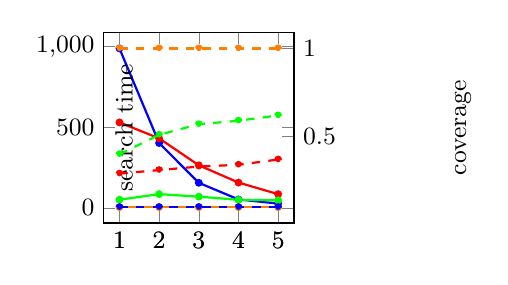
\begin{tikzpicture}
\small
    \begin{axis}[
    width = 4cm,
    height= 4cm,
    enlarge x limits = 0.1,
    enlarge y limits = 0.1,
    legend columns=3,
    legend style={at={(0.05,-0.3)},anchor=west},
    xmax = 5,
    xtick={1,2,3,4,5},
    xmin = 1,
	ylabel= search time,
	y label style={at={(0.2,0.5)}},
]

%blocksworld search time
\addplot[thick, blue, mark=*,
mark options={scale=0.5},
]
        plot coordinates {
			(1, 988.97)
			(2, 401.91)
			(3, 155.03)
			(4, 51.77)
			(5, 26.16)
        };

%nomystery search time
\addplot[thick, red, mark=*,
mark options={scale=0.5},
]
        plot coordinates {
			(1, 529.89)
			(2, 430.76)
			(3, 263.71)
			(4, 156.58)
			(5, 84.6)
        };

%tpp search time
\addplot[thick, green, mark=*, mark options={scale=0.5},
]
        plot coordinates {
			(1, 50.28)
			(2, 84.69)
			(3, 69.21)
			(4, 49.51)
			(5, 46.38)
        };


%rovers search time
\addplot[thick, orange, mark=*, mark options={scale=0.5},
]
        plot coordinates {
			(1, 4.17)
			(2, 4.17)
			(3, 4.17)
			(4, 4.17)
			(5, 4.17)
        };
\end{axis}

\begin{axis}[
    width = 4cm,
    height= 4cm,
    enlarge x limits = 0.1,
    enlarge y limits = 0.1,
    legend columns=3,
    legend style={at={(0.05,-0.3)},anchor=west},
    xmax = 5,
    xtick={1,2,3,4,5},
    xmin = 1,
	axis y line*=right,
	ylabel= coverage,
	y label style={at={(1.8,0.5)}},
]

%coverage blocksworld
\addplot[thick, blue, dashed, mark=*,
mark options={scale=0.5},
]
        plot coordinates {
			(1, 0.1)
			(2, 0.1)
			(3, 0.1)
			(4, 0.1)
			(5, 0.1)
        };

%coverage nomystery
\addplot[thick, red, dashed, mark=*,
mark options={scale=0.5},
]
        plot coordinates {
			(1, 0.29)
			(2, 0.31)
			(3, 0.33)
			(4, 0.34)
			(5, 0.37)
        };

%tpp coverage
\addplot[thick, green, dashed, mark=*, mark options={scale=0.5},
]
        plot coordinates {
			(1, 0.4)
			(2, 0.51)
			(3, 0.57)
			(4, 0.59)
			(5, 0.62)
        };

%rovers coverage
\addplot[thick, orange, dashed, mark=*, mark options={scale=0.5},
]
        plot coordinates {
			(1, 1.0)
			(2, 1.0)
			(3, 1.0)
			(4, 1.0)
			(5, 1.0)
        };

    \end{axis}


\end{tikzpicture}
%MUGS
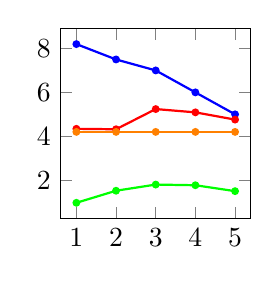
\begin{tikzpicture}

    \begin{axis}[
	%title = \#MUGS,
    width = 4cm,
    height= 4cm,
    enlarge x limits = 0.1,
    enlarge y limits = 0.1,
    legend columns=3,
    legend style={at={(0.05,-0.3)},anchor=west},
    xmax = 5,
    xtick={1,2,3,4,5},
    xmin = 1,
]

%MUGS blocksworld
\addplot[thick, blue, mark=*,
mark options={scale=0.5},
]
        plot coordinates {
			(1, 8.2)
			(2, 7.5)
			(3, 7.0)
			(4, 6.0)
			(5, 5.0)
        };

%MUGS nomystery
\addplot[thick, red, mark=*,
mark options={scale=0.5},
]
        plot coordinates {
			(1, 4.34)
			(2, 4.32)
			(3, 5.24)
			(4, 5.09)
			(5, 4.76)
        };


%MUGS TPP
\addplot[thick, green, mark=*, mark options={scale=0.5},
]
        plot coordinates {
			(1, 0.97)
			(2, 1.52)
			(3, 1.8)
			(4, 1.77)
			(5, 1.5)
        };

%MUGS TPP
\addplot[thick, orange, mark=*, mark options={scale=0.5},
]
        plot coordinates {
			(1, 4.2)
			(2, 4.2)
			(3, 4.2)
			(4, 4.2)
			(5, 4.2)

        };

\end{axis}
\end{tikzpicture}



%Search time
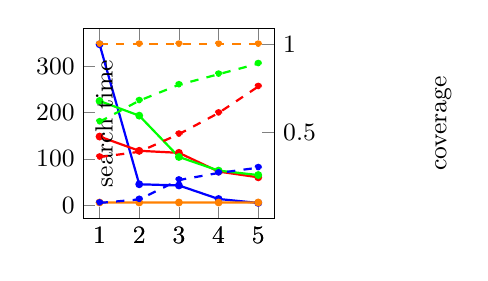
\begin{tikzpicture}
\small
    \begin{axis}[
    width = 4cm,
    height= 4cm,
    enlarge x limits = 0.1,
    enlarge y limits = 0.1,
    legend columns=3,
    legend style={at={(0.05,-0.3)},anchor=west},
    xmax = 5,
    xtick={1,2,3,4,5},
    xmin = 1,
	ylabel= search time,
	y label style={at={(0.2,0.5)}},
	axis y line*=left,
]

%blocksworld search time
\addplot[thick, blue, mark=*,
mark options={scale=0.5},
]
        plot coordinates {
			(1, 347.07)
			(2, 45.37)
			(3, 42.83)
			(4, 13.64)
			(5, 5.13)
        };

%nomystery search time
\addplot[thick, red, mark=*,
mark options={scale=0.5},
]
        plot coordinates {
			(1, 148.17)
			(2, 117.49)
			(3, 113.11)
			(4, 72.75)
			(5, 60.35)
        };

%tpp search time
\addplot[thick, green, mark=*, mark options={scale=0.5},
]
        plot coordinates {
			(1, 224.88)
			(2, 193.23)
			(3, 104.21)
			(4, 74.84)
			(5, 65.23)
        };


%rovers search time
\addplot[thick, orange, mark=*, mark options={scale=0.5},
]
        plot coordinates {
			(1, 6.09)
			(2, 6.12)
			(3, 6.12)
			(4, 6.11)
			(5, 6.1)
        };
\end{axis}

\begin{axis}[
    width = 4cm,
    height= 4cm,
    enlarge x limits = 0.1,
    enlarge y limits = 0.1,
    legend columns=3,
    legend style={at={(0.05,-0.3)},anchor=west},
    xmax = 5,
    xtick={1,2,3,4,5},
    xmin = 1,
	axis y line*=right,
	ylabel= coverage,
	y label style={at={(1.8,0.5)}},
]

%coverage blocksworld
\addplot[thick, blue, dashed, mark=*,
mark options={scale=0.5},
]
        plot coordinates {
			(1, 0.1)
			(2, 0.12)
			(3, 0.23)
			(4, 0.27)
			(5, 0.3)
        };

%coverage nomystery
\addplot[thick, red, dashed, mark=*,
mark options={scale=0.5},
]
        plot coordinates {
			(1, 0.36)
			(2, 0.39)
			(3, 0.49)
			(4, 0.61)
			(5, 0.76)
        };

%tpp coverage
\addplot[thick, green, dashed, mark=*, mark options={scale=0.5},
]
        plot coordinates {
			(1, 0.56)
			(2, 0.68)
			(3, 0.77)
			(4, 0.83)
			(5, 0.89)
        };

%rovers coverage
\addplot[thick, orange, dashed, mark=*, mark options={scale=0.5},
]
        plot coordinates {
			(1, 1.0)
			(2, 1.0)
			(3, 1.0)
			(4, 1.0)
			(5, 1.0)
        };

    \end{axis}


\end{tikzpicture}
%MUGS
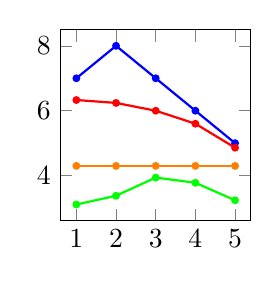
\begin{tikzpicture}

    \begin{axis}[
	%title = \#MUGS,
    width = 4cm,
    height= 4cm,
    enlarge x limits = 0.1,
    enlarge y limits = 0.1,
    legend columns=3,
    legend style={at={(0.05,-0.3)},anchor=west},
    xmax = 5,
    xtick={1,2,3,4,5},
    xmin = 1,
]

%MUGS blocksworld
\addplot[thick, blue, mark=*,
mark options={scale=0.5},
]
        plot coordinates {
			(1, 7.0)
			(2, 8.0)
			(3, 7.0)
			(4, 6.0)
			(5, 5.0)
        };

%MUGS nomystery
\addplot[thick, red, mark=*,
mark options={scale=0.5},
]
        plot coordinates {
			(1, 6.33)
			(2, 6.24)
			(3, 6.0)
			(4, 5.6)
			(5, 4.86)
        };


%MUGS TPP
\addplot[thick, green, mark=*, mark options={scale=0.5},
]
        plot coordinates {
			(1, 3.11)
			(2, 3.38)
			(3, 3.94)
			(4, 3.78)
			(5, 3.24)
        };

%MUGS rovers
\addplot[thick, orange, mark=*, mark options={scale=0.5},
]
        plot coordinates {
			(1, 4.3)
			(2, 4.3)
			(3, 4.3)
			(4, 4.3)
			(5, 4.3)
        };
\end{axis}
\end{tikzpicture}



%Search time
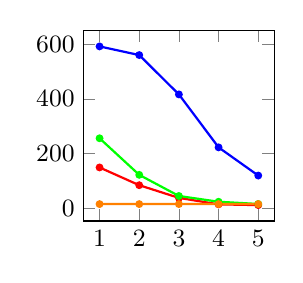
\begin{tikzpicture}
\small
    \begin{axis}[
    width = 4cm,
    height= 4cm,
    enlarge x limits = 0.1,
    enlarge y limits = 0.1,
    legend columns=3,
    legend style={at={(0.05,-0.3)},anchor=west},
    xmax = 5,
    xtick={1,2,3,4,5},
    xmin = 1,
	%ylabel= search time,
	y label style={at={(0.2,0.5)}},
	%axis y line*=left,
]

%blocksworld search time
\addplot[thick, blue, mark=*,
mark options={scale=0.5},
]
        plot coordinates {
			(1, 592.02)
			(2, 560.37)
			(3, 416.6)
			(4, 223.04)
			(5, 119.97)
        };

%nomystery search time
\addplot[thick, red, mark=*,
mark options={scale=0.5},
]
        plot coordinates {
			(1, 149.58)
			(2, 84.73)
			(3, 38.38)
			(4, 14.7)
			(5, 12.02)

        };

%tpp search time
\addplot[thick, green, mark=*, mark options={scale=0.5},
]
        plot coordinates {
			(1, 256.29)
			(2, 122.6)
			(3, 45.34)
			(4, 24.28)
			(5, 16.11)

        };


%rovers search time
\addplot[thick, orange, mark=*, mark options={scale=0.5},
]
        plot coordinates {
			(1, 15.72)
			(2, 15.7)
			(3, 15.7)
			(4, 15.72)
			(5, 15.71)
        };
\end{axis}

%\begin{axis}[
%    width = 4cm,
%    height= 4cm,
%    enlarge x limits = 0.1,
%    enlarge y limits = 0.1,
%    legend columns=3,
%    legend style={at={(0.05,-0.3)},anchor=west},
%    xmax = 5,
%    xtick={1,2,3,4,5},
%    xmin = 1,
%	axis y line*=right,
%	ylabel= coverage,
%	y label style={at={(1.8,0.5)}},
%	ytick={0,0.5,1},
%	ymin=0,
%	ymax=1,
%]
%
%%coverage blocksworld
%\addplot[thick, blue, dashed, mark=*,
%mark options={scale=0.5},
%]
%        plot coordinates {
%			(1, 0.31)
%			(2, 0.6)
%			(3, 0.87)
%			(4, 0.97)
%			(5, 1.0)
%        };
%
%%coverage nomystery
%\addplot[thick, red, dashed, mark=*,
%mark options={scale=0.5},
%]
%        plot coordinates {
%			(1, 0.81)
%			(2, 0.82)
%			(3, 0.82)
%			(4, 0.84)
%			(5, 0.9)
%        };
%
%%tpp coverage
%\addplot[thick, green, dashed, mark=*, mark options={scale=0.5},
%]
%        plot coordinates {
%			(1, 0.95)
%			(2, 1.0)
%			(3, 1.0)
%			(4, 1.0)
%			(5, 1.0)
%        };
%
%%rovers coverage
%\addplot[thick, orange, dashed, mark=*, mark options={scale=0.5},
%]
%        plot coordinates {
%			(1, 1.0)
%			(2, 1.0)
%			(3, 1.0)
%			(4, 1.0)
%			(5, 1.0)
%        };
%
%    \end{axis}


\end{tikzpicture}
%MUGS
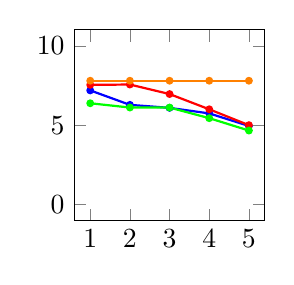
\begin{tikzpicture}

    \begin{axis}[
	%title = \#MUGS,
    width = 4cm,
    height= 4cm,
    enlarge x limits = 0.1,
    enlarge y limits = 0.1,
    legend columns=3,
    legend style={at={(0.05,-0.3)},anchor=west},
    xmax = 5,
    xtick={1,2,3,4,5},
    xmin = 1,
	xmax=5,
    ytick={0,5,10},
	ymin=0,
	ymax=10,
]

%MUGS blocksworld
\addplot[thick, blue, mark=*,
mark options={scale=0.5},
]
        plot coordinates {
			(1, 7.19)
			(2, 6.28)
			(3, 6.09)
			(4, 5.74)
			(5, 4.95)

        };

%MUGS nomystery
\addplot[thick, red, mark=*,
mark options={scale=0.5},
]
        plot coordinates {
			 (1, 7.54)
			(2, 7.56)
			(3, 6.96)
			(4, 6.0)
			(5, 5.0)

        };


%MUGS TPP
\addplot[thick, green, mark=*, mark options={scale=0.5},
]
        plot coordinates {
			(1, 6.38)
			(2, 6.11)
			(3, 6.11)
			(4, 5.44)
			(5, 4.66)

        };

%MUGS rovers
\addplot[thick, orange, mark=*, mark options={scale=0.5},
]
        plot coordinates {
			(1, 7.8)
			(2, 7.8)
			(3, 7.8)
			(4, 7.8)
			(5, 7.8)
        };
\end{axis}
\end{tikzpicture}



%\rebecca{top c=1.25, bottom c = 1.0}
\vspace{-0.3cm}
\caption{\label{fig:asp-local} Local action-set property explanation 
results for SysS as a function of $|A|$. Coverage and average runtime
(left), average \#MUGS (right). Blocksworld blue, NoMystery red, Rovers orange, TPP green. 
\joerg{integrate reference point coverage as horizontal lines into the left plot} 
\rebecca{lmcut and tarp ref always 1.0 coverage}
}
%
%\caption{$c = 1.25$ red: nomyters (5 goals, 5 props), green: TPP (7 goals, 9 props), left plot: search time and coverage, right plot: \#MUGS}
%
\vspace{-0.2cm}
\end{figure}



%%%% Action-Set Properties, END SUBMISSION VERSION
%%%%%%%%%%%%%%%%%%%%%%%%%%%%%%%%%%%%%%%%%%%%%%%%%%%%%%%%%%%%%%%%%%%%
%%%%%%%%%%%%%%%%%%%%%%%%%%%%%%%%%%%%%%%%%%%%%%%%%%%%%%%%%%%%%%%%%%%%
%%%%%%%%%%%%%%%%%%%%%%%%%%%%%%%%%%%%%%%%%%%%%%%%%%%%%%%%%%%%%%%%%%%%







%%%%%%%%%%%%%%%%%%%%%%%%%%%%%%%%%%%%%%%%%%%%%%%%%%%%%%%%%%%%%%%%%%%%
%%%%%%%%%%%%%%%%%%%%%%%%%%%%%%%%%%%%%%%%%%%%%%%%%%%%%%%%%%%%%%%%%%%%
%%%%%%%%%%%%%%%%%%%%%%%%%%%%%%%%%%%%%%%%%%%%%%%%%%%%%%%%%%%%%%%%%%%%
%%%% PRE-FINAL AND SUPPLEMENTARY MATERIAL VERSION

\ifdefined\suppflagdefined

\subsection{Action-Set Properties}

\begin{figure*}[htb]
\centering\centering
%\newlength{\mywidth}
\setlength{\mywidth}{16.5cm}

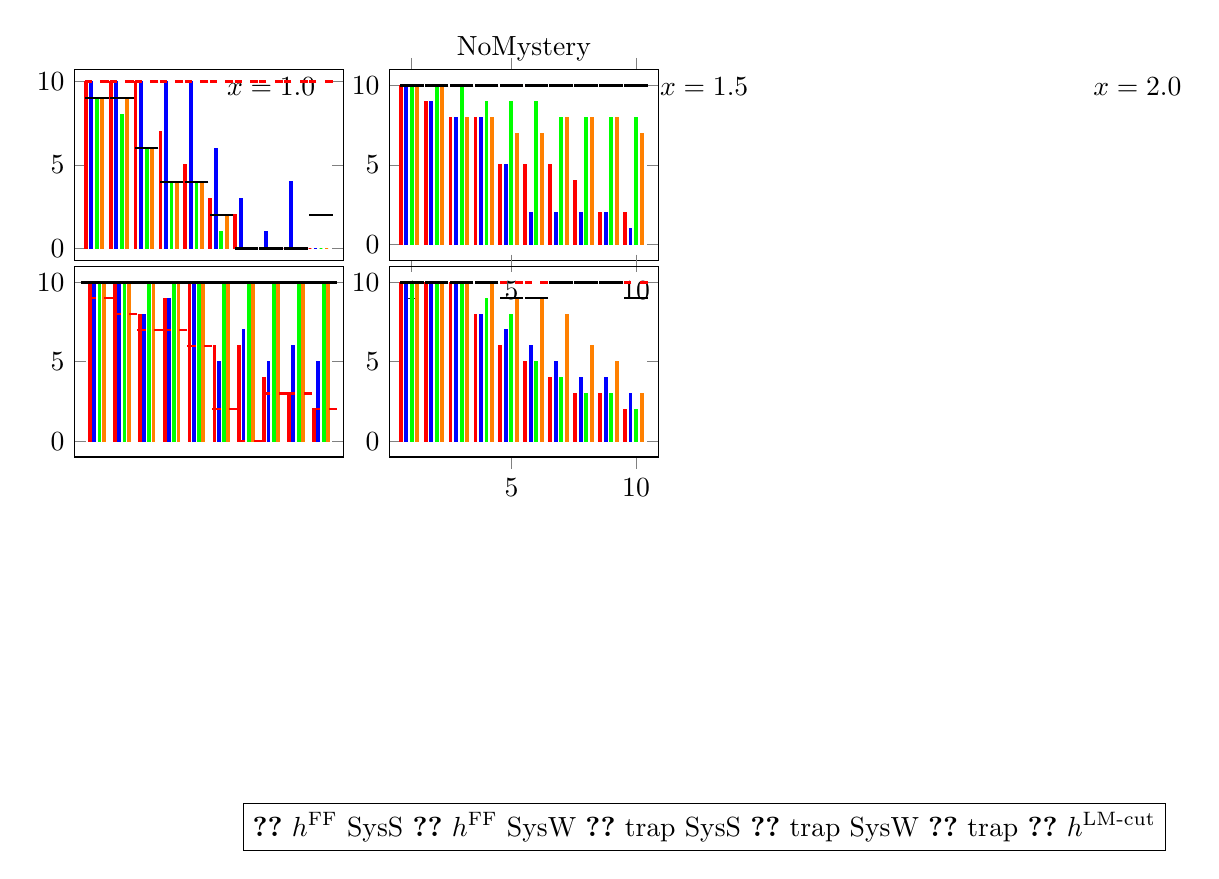
\begin{tikzpicture}
\node[] (c1) at (2.5,2.2) {$x=1.0$};
\node[] (c15) at (8,2.2) {$x=1.5$};
\node[] (c2) at (13.5,2.2) {$x=2.0$};


    \begin{axis}[
    width = 5cm,
    height=4cm,
    enlarge x limits = 0.1,
    enlarge y limits = 0.07,
    legend columns=1,
    ybar,
    bar width=1pt,
    ymin = 0,
    ymax = 10,
	compat=1.6,
	title={},
	xticklabels={,,},
	xtick style={draw=none},
	%ylabel=goals 06,
	at={(0,0)},
]
\addplot+[ybar, bar shift =-4.0pt, red,
]
plot coordinates {
(07, 2) %c_125
(08, 0) %c_125
(03, 10) %c_125
(10, 0) %c_125
(06, 3) %c_125
(09, 0) %c_125
(02, 10) %c_125
(05, 5) %c_125
(04, 7) %c_125
(01, 10) %c_125
};
\label{plot:props_hff_bu_53}
\addplot+[ybar, bar shift =-2.0pt, blue,
]
plot coordinates {
(07, 3) %c_125
(08, 1) %c_125
(03, 10) %c_125
(10, 0) %c_125
(06, 6) %c_125
(09, 4) %c_125
(02, 10) %c_125
(05, 10) %c_125
(04, 10) %c_125
(01, 10) %c_125
};
\label{plot:props_hff_td_53}
\addplot+[ybar, bar shift =0.0pt, green,
]
plot coordinates {
(07, 0) %c_125
(08, 0) %c_125
(03, 6) %c_125
(10, 0) %c_125
(06, 1) %c_125
(09, 0) %c_125
(02, 8) %c_125
(05, 4) %c_125
(04, 4) %c_125
(01, 9) %c_125
};
\label{plot:props_trap_bu_53}
\addplot+[ybar, bar shift =2.0pt, orange,
]
plot coordinates {
(07, 0) %c_125
(08, 0) %c_125
(03, 6) %c_125
(10, 0) %c_125
(06, 2) %c_125
(09, 0) %c_125
(02, 9) %c_125
(05, 4) %c_125
(04, 4) %c_125
(01, 9) %c_125
};
\label{plot:props_trap_td_53}

%lmcut
\addplot+[only marks, mark = -, mark options = {thick, red, dashed}, mark size = 0.15cm, black,
]
plot coordinates {
(02, 10)
(01, 10)
(04, 10)
(03, 10)
(07, 10)
(08, 10)
(06, 10)
(10, 10)
(05, 10)
(09, 10)
};

%trap first meta node top down
\addplot+[only marks, mark = -, mark options = {thick, black}, mark size = 0.15cm, black,
]
plot coordinates {
(01, 9)
(02, 9)
(03, 6)
(04, 4)
(05, 4)
(06, 2)
(07, 0)
(08, 0)
(09, 0)
(10, 2)
};
    \end{axis}
    \hfill
    
%\node[draw, align=center] (test) at (2,-2) {
%\ref{plot:props_hff_bu_53} props-hff-bu\\
%\ref{plot:props_hff_td_53} props-hff-td\\
%\ref{plot:props_trap_bu_53} props-trap-bu\\
%\ref{plot:props_trap_td_53} props-trap-td\\
%};



    \begin{axis}[
    width = 5cm,
    height=4cm,
    enlarge x limits = 0.1,
    enlarge y limits = 0.1,
    legend columns=1,
    ybar,
    bar width=1pt,
    ymin = 0,
    ymax = 10,
	compat=1.6,
	title=NoMystery,
	title style={yshift=-1.5ex},
	%ylabel=goals 6,
	%xticklabels={,,},
	%xtick style={draw=none},
	xtick= {1,5,10},
	at={(4cm,0)},
]
\addplot+[ybar, bar shift =-4.0pt, red,
]
plot coordinates {
(04, 8) %c_100
(09, 2) %c_100
(10, 2) %c_100
(08, 4) %c_100
(02, 9) %c_100
(07, 5) %c_100
(06, 5) %c_100
(05, 5) %c_100
(03, 8) %c_100
(01, 10) %c_100
};
\label{plot:props_bu_hff_46}
\addplot+[ybar, bar shift =-2.0pt, blue,
]
plot coordinates {
(04, 8) %c_100
(09, 2) %c_100
(10, 1) %c_100
(08, 2) %c_100
(02, 9) %c_100
(07, 2) %c_100
(06, 2) %c_100
(05, 5) %c_100
(03, 8) %c_100
(01, 10) %c_100
};
\label{plot:props_td_hff_46}
\addplot+[ybar, bar shift =0.0pt, green,
]
plot coordinates {
(04, 9) %c_100
(09, 8) %c_100
(10, 8) %c_100
(08, 8) %c_100
(02, 10) %c_100
(07, 8) %c_100
(06, 9) %c_100
(05, 9) %c_100
(03, 10) %c_100
(01, 10) %c_100
};
\label{plot:props_bu_trap_46}
\addplot+[ybar, bar shift =2.0pt, orange,
]
plot coordinates {
(04, 8) %c_100
(09, 8) %c_100
(03, 8) %c_100
(08, 8) %c_100
(02, 10) %c_100
(07, 8) %c_100
(06, 7) %c_100
(05, 7) %c_100
(10, 7) %c_100
(01, 10) %c_100
};
\label{plot:props_td_trap_46}

%lmcut
\addplot+[only marks, mark = -, mark options = {thick, red, dashed}, mark size = 0.15cm, black,
]
plot coordinates {
(01, 10)
(02, 10)
(03, 10)
(04, 10)
(05, 10)
(06, 10)
(07, 10)
(08, 10)
(09, 10)
(10, 10)
};

%trap first meta node top down
\addplot+[only marks, mark = -, mark options = {thick, black}, mark size = 0.15cm, black,
]
plot coordinates {
(01, 10)
(02, 10)
(03, 10)
(04, 10)
(05, 10)
(06, 10)
(07, 10)
(08, 10)
(09, 10)
(10, 10)
};
    \end{axis}
    \hfill
    
%\node[draw, align=center] (test) at (8,-18) {
%\ref{plot:props_bu_hff_46} props-bu-hff\\
%\ref{plot:props_td_hff_46} props-td-hff\\
%\ref{plot:props_bu_trap_46} props-bu-trap\\
%\ref{plot:props_td_trap_46} props-td-trap\\
%};



\begin{axis}[
width = 5cm,
height=4cm,
enlarge x limits = 0.1,
enlarge y limits = 0.1,
legend columns=1,
ybar,
bar width=1pt,
ymin = 0,
ymax = 10,
compat=1.6,
at={(0,-2.5cm)},
	xticklabels={,,},
	xtick style={draw=none},
]
\addplot+[ybar, bar shift =-2.5pt, red,
]
plot coordinates {
(08, 4)
(09, 3)
(01, 10)
(03, 8)
(02, 10)
(04, 9)
(05, 10)
(06, 6)
(10, 2)
(07, 6)
};
\label{plot:properties_hff_bu_52}
\addplot+[ybar, bar shift =-1.0pt, blue,
]
plot coordinates {
(01, 10)
(08, 5)
(02, 10)
(04, 9)
(03, 8)
(05, 10)
(06, 5)
(10, 5)
(07, 7)
(09, 6)
};
\label{plot:properties_hff_td_52}
\addplot+[ybar, bar shift =1.0pt, green,
]
plot coordinates {
(09, 10)
(01, 10)
(02, 10)
(04, 10)
(03, 10)
(05, 10)
(06, 10)
(10, 10)
(07, 10)
(08, 10)
};
\label{plot:properties_trap_prefop_bu_52}
\addplot+[ybar, bar shift =2.5pt, orange,
]
plot coordinates {
(01, 10)
(08, 10)
(02, 10)
(03, 10)
(04, 10)
(05, 10)
(06, 10)
(10, 10)
(07, 10)
(09, 10)
};
\label{plot:properties_trap_prefop_td_52}

%start node sysW
\addplot+[only marks, mark = -, mark options = {thick}, mark size = 0.2cm, black,
]
plot coordinates {
(02, 10)
(01, 10)
(04, 10)
(03, 10)
(07, 10)
(08, 10)
(06, 10)
(10, 10)
(05, 10)
(09, 10)
};
%optimal
\addplot+[only marks, mark = -, mark options = {thick, red, dashed}, mark size = 0.2cm, black,
]
plot coordinates {
(03, 7)
(05, 6)
(07, 0)
(09, 3)
(01, 9)
(02, 8)
(04, 7)
(06, 2)
(08, 3)
(10, 2)
};

\end{axis}


    \begin{axis}[
    width = 5cm,
    height=4cm,
    enlarge x limits = 0.1,
    enlarge y limits = 0.1,
    legend columns=1,
    ybar,
    bar width=1pt,
    ymin = 0,
    ymax = 10,
compat=1.6,
%title=c 150,
%ylabel=goals 7,
at={(4cm,-2.5cm)},
]
\addplot+[ybar, bar shift =-4.0pt, red,
]
plot coordinates {
(07, 4) %c_150
(06, 5) %c_150
(05, 6) %c_150
(09, 3) %c_150
(08, 3) %c_150
(10, 2) %c_150
(01, 10) %c_150
(04, 8) %c_150
(03, 10) %c_150
(02, 10) %c_150
};
\label{plot:props_bu_hff_49}
\addplot+[ybar, bar shift =-2.0pt, blue,
]
plot coordinates {
(07, 5) %c_150
(06, 6) %c_150
(05, 7) %c_150
(09, 4) %c_150
(08, 4) %c_150
(10, 3) %c_150
(01, 10) %c_150
(04, 8) %c_150
(03, 10) %c_150
(02, 10) %c_150
};
\label{plot:props_td_hff_49}
\addplot+[ybar, bar shift =0.0pt, green,
]
plot coordinates {
(07, 4) %c_150
(06, 5) %c_150
(05, 8) %c_150
(09, 3) %c_150
(08, 3) %c_150
(03, 10) %c_150
(01, 10) %c_150
(04, 9) %c_150
(10, 2) %c_150
(02, 10) %c_150
};
\label{plot:props_bu_trap_49}
\addplot+[ybar, bar shift =2.0pt, orange,
]
plot coordinates {
(07, 8) %c_150
(06, 9) %c_150
(05, 9) %c_150
(09, 5) %c_150
(08, 6) %c_150
(10, 3) %c_150
(01, 10) %c_150
(04, 10) %c_150
(03, 10) %c_150
(02, 10) %c_150
};
\label{plot:props_td_trap_49}

%lmcut
\addplot+[only marks, mark = -, mark options = {thick, red, dashed}, mark size = 0.15cm, black,
]
plot coordinates {
(02, 10)
(01, 10)
(04, 10)
(03, 10)
(07, 10)
(08, 10)
(06, 10)
(10, 10)
(05, 10)
(09, 10)
};

%trap first meta node top down
\addplot+[only marks, mark = -, mark options = {thick, black}, mark size = 0.15cm, black,
]
plot coordinates {
(01, 10)
(02, 10)
(03, 10)
(04, 10)
(05, 9)
(06, 9)
(07, 10)
(08, 10)
(09, 10)
(10, 9)
};
    \end{axis}
    \hfill
    
%\node[draw, align=center] (test) at (8,-18) {
%\ref{plot:props_bu_hff_49} props-bu-hff\\
%\ref{plot:props_td_hff_49} props-td-hff\\
%\ref{plot:props_bu_trap_49} props-bu-trap\\
%\ref{plot:props_td_trap_49} props-td-trap\\
%};



\node[draw] (test) at (8,-7.2) {
\ref{plot:properties_hff_bu_39} $\hff$ SysS
\ref{plot:properties_hff_td_39} $\hff$ SysW
\ref{plot:properties_trap_prefop_bu_39} trap SysS
\ref{plot:properties_trap_prefop_td_39} trap SysW
\ref{plot:baseline_sysW_node} trap
\ref{plot:baseline_lmcut} \hlmcut
};
\end{tikzpicture}

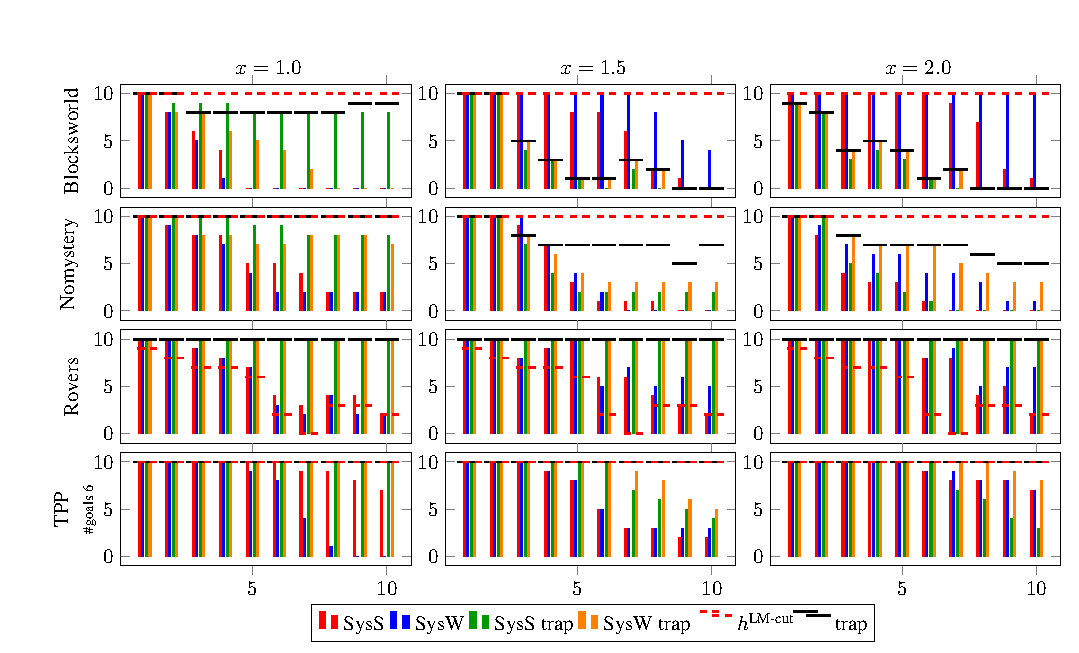
\includegraphics{data/action_set_properties/barchart/barchart.pdf}
\vspace{-0.6cm}
\caption{Coverage results on IPC benchmarks extended with action-set properties.}
\label{fig:barcharts}
\vspace{-0.2cm}
\end{figure*}

To evaluate the use of our framework with more complex plan
properties, beyond goal facts, we experimented with the compilation of
action-set properties as per Section~\ref{compilation}. We selected
four IPC domains for extension with action-set properties, namely
NoMystery, Rovers, and TPP as considered in resource-constrained
planning \cite{nakhost:etal:icaps-12}, where minimum resource
requirements are known as per available problem generators; plus the
Blocksworld as an intuitively rather differently structured domain. In
all four domains, we use discrete resource consumption encoded into
the STRIPS model, enabling the use of trap
learning \cite{steinmetz:hoffmann:ijcai-17} which turns out to be
highly beneficial here.

In Blocksworld, we include two gripper hands and the action-set
properties ask whether a given gripper is used to pick up a given
block, or to stack a given pair of blocks. In NoMystery, the
properties are as in our illustrative example
(Section~\ref{illustrative-example}). In Rovers, the properties ask
whether a given rover or camera is used for a given observation. In
TPP, they ask whether given road segments are used, and whether given
goods are bought at given markets. In all cases, we vary the number of
action-set properties between 1 and 10. We fix the original goal facts
as hard goals, and we set the available resources to $x \in \{1.0,1.5,
2.0\}$ times the minimum needed to allow for costlier plans satisfying
some of the properties.

We created benchmark tasks with size parameters around the borderline
of computational feasibility for our analyses, given our time/memory
limits. In Blocksworld, we used 5 -- 8 blocks; in NoMystery, our tasks
have 2 trucks, 6 locations, and 4 -- 7 packages; in Rovers, they have
2 rovers, 5 waypoints, and 4 -- 7 science objectives; in TPP, we use 5
markets, 1 depot, and 4 -- 7 goods. In all domains, we vary the number
of goal facts (and associated objects) between 4 and 7. We create 10
base instances for each size-parameter setting, which are then
modified for our experiments with different initial resource levels,
and action-set properties to be considered.
%
%% \begin{enumerate}
%% \item The resource constrained \textit{rovers} domain. Problems were generated with 2 rovers, 5 waypoints. Action properties are to use a specific rover for a sample or an observation, or to use a specific camera for an observation. 
%% \item The \textit{blocksworld} domain with 2 grippers, modified such that picking up or unstacking a block costs high or low energy depending upon which gripper is used. Problems were generated scaling from 3 to 10 blocks. Action properties are to use a specific gripper to pick up a specific block, or to use any gripper to stack a specific pair of blocks at any point in the plan.
%% \item The resource constrained \textit{TPP} domain. Problems were generated with 5 markets and 1 depot. Properties are to use or not use particular road segments, and preferred markets for goods.
%% \item The resource constrained \textit{nomystery} domain, described in the example. Problems were generated with 6 locations and 2 trucks.
%% \end{enumerate}

To have some comparison measure for performance, again we use
classical-planning reference points, based on \astar\ with \hlmcut,
and on search with trap learning, respectively. We now run these
reference points on tasks where all (original goal facts plus)
action-set properties are hard goals. These tasks may be solvable (in
which case \astar\ with \hlmcut\ tends to be better) or unsolvable (in
which case trap learning tends to be better). The configurations of
our own algorithm are SysS and SysW as before, now with vs.\ without
trap learning (and transfer).

Figure~\ref{fig:barcharts} shows the coverage data. To give an
overview, we show one row per domain, fixing the number of hard goals
at the feasibility borderline. Smaller numbers of goal facts tend to
be quite easy, larger ones mostly infeasible, with variance depending
on the domain and algorithm.
Appendix~\ref{data-action-set-properties} gives complete data for each
of the four domains.

In Blocksworld, the best of our techniques are moderately competitive
with the \hlmcut\ reference point (which starts to lose coverage when
one more block is added). They match the performance of the other
reference point for $x=1.0$, and surpass it for larger $x$ where trap
learning incurs a prohibitive overhead. NoMystery is the most
problematic domain in terms of performance, with all our techniques
lagging far behind the two reference points. In Rovers,
though, \astar\ with \hlmcut\ is much less effective than our
techniques, which match the full coverage of the trap-learning
reference point. TPP is similar to Blocksworld in that our techniques
are moderately competitive with the reference points. 
%\joerg{statement where coverage for these starts to go down} 
Trap learning is highly
beneficial in all cases except Blocksworld with $x>1.0$. Overall, it
seems fair to say that our action-set property dependency analysis is
not exceedingly infeasible compared to related classical planning
problems.


\fi

%%%% END PRE-FINAL AND SUPPLEMENTARY MATERIAL VERSION
%%%%%%%%%%%%%%%%%%%%%%%%%%%%%%%%%%%%%%%%%%%%%%%%%%%%%%%%%%%%%%%%%%%%
%%%%%%%%%%%%%%%%%%%%%%%%%%%%%%%%%%%%%%%%%%%%%%%%%%%%%%%%%%%%%%%%%%%%
%%%%%%%%%%%%%%%%%%%%%%%%%%%%%%%%%%%%%%%%%%%%%%%%%%%%%%%%%%%%%%%%%%%%



\FloatBarrier

\section{Other Related Works}
\label{related}

%% \joerg{0.5 pages. TBD if we need this. Given the ijcai feedback, I
%%   tend to think that yes. briefly summarize key points mentioned
%%   before; and discuss any other relations not discussed before due
%%   to text flow/or give more details on things that were
%%   mentioned. XAIP, OSP, conflict analysis, domain analysis, model
%%   checking.}

%% I normally don't include sections like this, as I find them boring;
%%   I usually just cover the brod literature context in the intro,
%%   and specific relations at those technical places where they are
%%   pertinent. Here though, matters may be different in that, in the
%%   intro, we can and should only spin the stroy for XAIP and perhaps
%%   domain analysis; while at the technical level people may wonder
%%   if what we do here concretely is not just a work on
%%   oversubscription planning. So we may want to add a section here
%%   discussing technical and conceptual relations to works -- in
%%   oversubscription planning, and also in conflict analysis see
%%   pointers below -- which are not naturally part of the XAIP story
%%   in the intro. ... TBD when writing the introduction}

Various works relate to our computation of MUGS. In SAT and CP,
minimal unsatisfiable cores (MUC,
\eg\ \cite{chinneck:2007,laborie:ecai-14}) are related to MUGS, yet
rely on constraint-conflict analysis and are non-exhaustive, \ie, do
not aim at finding \emph{all} MUCs. Similarly, in the temporal planner
IxTeT, an analysis of resource conflicts finds minimal critical sets
(effects over-consuming a resource)
\cite{laborie:ghallab:ijcai-95}. On the exhaustive side, problems and
algorithms involving some form of solvability borderline within a
lattice of problem variants have been considered since a long time
(\eg\ \cite{dekleer:ai-86:atms,reiter:ai-87}). In particular, the
diagnosis framework by Grastien et
al.\ \shortcite{grastien:etal:dx-11,grastien:etal:kr-12} can cast
maximum solvable goal subsets as preferred diagnoses. That work uses
SAT instead of a base planner, but an encoding into planning has been
devised and ideas for search enhancements may be transferrable.
%
% between the two algorithms (in both directions).

Some prior work \cite{yu:etal:jair-17,lauffer:topcu:xaip-19} aims at
suggesting goals to drop in oversubscribed situations, through
conflict analyses related to finding a MUGS. At the technical level,
both works are quite different from ours though as they use
constraint-based problem encodings.

Prior work on other forms of plan-space explanation addressed
unsolvable tasks, identifying minimal model changes resulting in
solvability \cite{goebelbecker:etal:icaps-10}, or minimal differences
between a solvable user model vs.\ unsolvable system model
\cite{sreedharan:etal:ijcai-19}.
%
% joerg: not needed, may be controversial (compilations etc)
%
%In contrast to these, here we are concerned with the space of plans in
%solvable tasks.

We remark that our approach can be viewed as a form of domain/task
analysis, or as a form of model checking applied to planning
models. Both have been explored before, but addressing very different
problems
(\eg\ \cite{fox:long:jair-98,rintanen:aaai-00,vaquero:etal:keq-13}).
%
%% % joerg: mention only briefly, ijcai reviewers did not complain about
%% % this anyway
%% %
%% %% An alternate view of our approach is as a form of domain analysis
%% %% (actually: task analysis), identifying particular properties of plan
%% %% space ahead of time. Indeed, various popular task analyses can be cast
%% %% as instances of our framework. A fact pair $(p,q)$ is mutually
%% %% exclusive \cite{blum:furst:ai-97} iff $p$-true-at-end entails $\neg
%% %% q$-true-at-end in the space of all applicable action sequences; a fact
%% %% $p$ is a landmark \cite{hoffmann:etal:jair-04} iff $\true$ entails
%% %% $p$-true-at-some-point; other examples presumably exist. From this
%% %% point of view, we generalize previous concepts to a broader
%% %% perspective aimed at addressing arbitrary user questions. 
%
%% %% At the same time, our approach itself can be viewed as an instance of
%% %% model checking of planning models
%% %% \cite{clarke:etal:01},\footnote{There has been little work on this
%% %%   subject; Vaquero et al.\ \shortcite{vaquero:etal:keq-13} use Petri
%% %%   nets to capture and check dynamic aspects of planning models in
%% %%   itSIMPLE.}  systematically checking all entailments between plan
%% %% properties. Again the value of our framework lies in its suitability
%% %% for XAIP (plus computational gains from considering all
%% %% \props\ dependencies in unison rather than running individual
%% %% entailment checks).


















%%%%%%%%%%%%%%%%%%%%%%%%%%%%%%%%%%%%%%%%%%%%%%%%%%%%%%%%%%%%%%%%%%%%%%%%%%
%%%%%%%%%%%%%%%%%%%%%%%%%%%%%%%%%%%%%%%%%%%%%%%%%%%%%%%%%%%%%%%%%%%%%%%%%%
%%%%%%%%%%%%%%%%%%%%%%%%%%%%%%%%%%%%%%%%%%%%%%%%%%%%%%%%%%%%%%%%%%%%%%%%%%

%% \joerg{previous text snippets:}

%% %% Related work by Brian Williams (need to find citations): reasoning
%% %% about user goals; oversubscription planning in constraint-based
%% %% planning formulation; suggest goals to drop based on conflict
%% %% analysis; constructive procedure to find these goals, given commitment
%% %% (subset of goals) and most important implications (subsets of other
%% %% goals dropping which makes the whole thing consistent ie goal
%% %% achievable). In short, the service provided is related to that
%% %% provided by our goalfact dependency analysis; but in a
%% %% direct/constructive manner, as opposed to our meta search tree, as
%% %% enabled by working in a constraint formulation and building on
%% %% conflict analysis in that setting.
%% %
%% %% Identifying the trade-off between soft goals in an iterative
%% %% oversubscription planning process relates, in terms of purpose, to
%% %% the work by Yu et al.\ \cite{yu:etal:jair-17}. A major difference
%% %% is that Yu et al.\ address conditional temporal problems, a form of
%% %% conditional temporal plans, instead of PDDL-style compactly
%% %% specified general planning problems. This more restricted focus
%% %% allows to leverage previous conflict analysis methods in that
%% %% area. It remains a question for future work whether such conflict
%% %% analysis could inspire more effective analysis methods in our
%% %% framework.


%% Yu et al.\ \shortcite{yu:etal:jair-17} perform an analysis suggesting
%% goals to drop in oversubscribed situations. This can be viewed as a
%% use of MUGS complementary to ours. At the technical level, our work is
%% quite different as Yu et al.\ address conditional temporal problems, a
%% form of constraint-based planning, and leverage previous conflict
%% analysis methods in that area. Similarly, Lauffer and Topcu
%% \shortcite{lauffer:topcu:xaip-19} perform conflict analysis on
%% oversubscribed scheduling problems.


%% %% \joerg{discuss relation to domain analysis / model checking?
%% %%   basically, our approach can be viewed as a form of domain analysis
%% %%   checking the truth of formulas over plan space. it seems to me that
%% %%   ``domain analysis'' should definitely be mentioned in our
%% %%   introduction, as another frame of reference besides
%% %%   XAIP. ... regarding model checking, our analysis can be viewed as a
%% %%   systematic form of checking a set of properties of interest; we
%% %%   structure this form of analysis as makes sense in explainable
%% %%   planning; computationally we exploit synergies in addressing the
%% %%   entire set of properties rather than checking each possible
%% %%   dependency in isolation; in the long-term, a highly relevant
%% %%   research line is how to discover relevant properties in the first
%% %%   place. ... as a concrete literature link, I know that some people
%% %%   from Brasil worked on using model checkers as a domaiun analysis
%% %%   tool, in the ICKEPS context; but I don't have the concrete
%% %%   references in mind/ don't know whether and where this has been
%% %%   published. ... we could perhaps mention in this context (currently
%% %%   mentioned in my text snippet below, but this could be moved
%% %%   elsewhere) that ultimately one may want to identify interesting plan
%% %%   properties automatically, which is then clearly beyond anything
%% %%   addressed in model checking.}
%% %


%% %% We remark that our approach can be viewed as a generalization of
%% %% domain/task analysis (as done \eg\ by \cite{fox:long:jair-98}), and as
%% %% an instance of model checking applied to planning models (related
%% %% \eg\ to \cite{vaquero:etal:keq-13}). Our contribution lies in
%% %% introducing this intermediate problem suited to XAIP as outlined, and
%% %% instantiating that formulation with initial technology showing promise
%% %% in practice.
%
%% Another alternate view of our approach is as a form of domain analysis
%% (actually: task analysis), identifying particular properties of plan
%% space ahead of time. Indeed, various popular task analyses can be cast
%% as instances of our framework. A fact pair $(p,q)$ is mutually
%% exclusive \cite{blum:furst:ai-97} iff $p$-true-at-end entails $\neg
%% q$-true-at-end in the space of all applicable action sequences; a fact
%% $p$ is a landmark \cite{hoffmann:etal:jair-04} iff $\true$ entails
%% $p$-true-at-some-point; other examples presumably exist. From this
%% point of view, we generalize previous concepts to a broader
%% perspective aimed at addressing arbitrary user questions. At the same
%% time, our approach itself can be viewed as an instance of model
%% checking of planning models \cite{clarke:etal:01},\footnote{There has
%%   been little work on this subject; Vaquero et
%%   al.\ \shortcite{vaquero:etal:keq-13} use Petri nets to capture and
%%   check dynamic aspects of planning models in itSIMPLE.}
%% systematically checking all entailments between plan properties. Again
%% the value of our framework lies in its suitability for XAIP (plus
%% computational gains from considering all \props\ dependencies in
%% unison rather than running individual entailment checks).
%
%% Identifying the trade-off between soft goals in an iterative
%% oversubscription planning process relates, in terms of purpose, to the
%% work by Yu et al.\ \cite{yu:etal:jair-17}. A major difference is that
%% Yu et al.\ address conditional temporal problems, a form of
%% conditional temporal plans, instead of PDDL-style compactly specified
%% general planning problems. This more restricted focus allows to
%% leverage previous conflict analysis methods in that area. It remains a
%% question for future work whether such conflict analysis could inspire
%% more effective analysis methods in our framework.


\section{Conclusion}
\label{conclusion}

\rebecca{Joerg}



\section{Examples}

\subsection{Nomystery}

\subsubsection*{Explanation Domain}
The goal in nomystery is to deliver packages from a initial location (labeled in red)
to a goal location (labeled in green). There are two trucks with a separate fuel level.
The amount of packages a truck can transport is not limited. A truck can either load or 
unload a package or drive from one to an other location. Loading and unloading costs no fuel,
driving costs between 1 and 5 fuels units (label at the edges).\\

Properties:
\begin{itemize}
	\item don't use $T_i$ $(L_x,L_y)$: Truck $T_i$ should not drive from $L_x$ to
		$L_y$ or vise versa
	\item use $T_i$ $(L_x,L_y)$: Truck $T_i$ should drive at least once from $L_x$ to
		$L_y$ or vise versa
	\item same truck $P_x$ $P_y$: both packages have to be delivered by the same truck
		(the packages are either only loaded and an unloaded by truck $T_0$ or by $T_1$)
\end{itemize}

\subsubsection*{Example 1}
%\begin{figure}
	The fuel limit is 1.5 times the minimal limit to deliver all packages.

	Initial fuel:
	$fuel(T_0) = 16$, $fuel(T_1) = 7$

	\begin{center}
	\begin{tikzpicture}
		\node[draw, circle, label=above:{\textcolor{red}{$P_0, P_1,P_2$}}] (l0) at (0,0) {$L_0$};
		\node[draw, circle, label=right:{$T_1$}] (l1) at (4,-1) {$L_1$};
		\node[draw, circle] (l2) at (6,0) {$L_2$};
		\node[draw, circle, label=right:{\textcolor{darkgreen}{$P_1$}}] (l3) at (6,-3) {$L_3$};
		\node[draw, circle, label=below:{\textcolor{darkgreen}{$P_0$}}] (l4) at (2,-2) {$L_4$};
		\node[draw, circle, label=below:{$T_0$ \textcolor{darkgreen}{$P_2$}}] (l5) at (0,-3) {$L_5$};

		\draw[thick] (l0) to node[above] {5} (l2);
		\draw[thick] (l0) to node[above] {2} (l1);
		\draw[thick] (l0) to node[above] {3} (l4);
		\draw[thick] (l0) to node[left] {4} (l5);
		\draw[thick] (l2) to node[right] {1} (l3);
		\draw[thick] (l4) to node[above] {2} (l1);
		\draw[thick] (l4) to node[above] {5} (l3);
		\draw[thick] (l5) to node[below] {5} (l3);
		\draw[thick] (l4) to node[below] {4} (l5);
	\end{tikzpicture}
	\end{center}
	\begin{minipage}[t]{0.3\textwidth}
	Properties:
	\begin{enumerate}
		\item use $T_0$ $(L_2,L_3)$
		\item same truck $P_1$ $P_2$
		\item use $T_0$ $(L_4,L_3)$
		\item same truck $P_2$ $P_0$
		\item don't use $T_0$ $(L_0,L_5)$
		\item use $T_1$ $(L_5,L_4)$
	\end{enumerate}
	\end{minipage}
	\begin{minipage}[t]{0.15\textwidth}
		MUGS:
		\begin{itemize}
			\item $\{4,5,6\}$
			\item $\{2,5,6\}$
			\item $\{3,4,5\}$
			\item $\{3,4,5\}$
			\item $\{2,4,5\}$
			\item $\{2,3,5\}$
			\item $\{1,3,4\}$
			\item $\{1,2,3\}$
		\end{itemize}
	\end{minipage}

\subsection{Blocksworld}

The cost bound is set to 11, 0.5 times the minimal cost to solve all goals.
You can pick up and put down a block from the table and stack and unstack two blocks.
Each of these actions costs 1.

\begin{center}
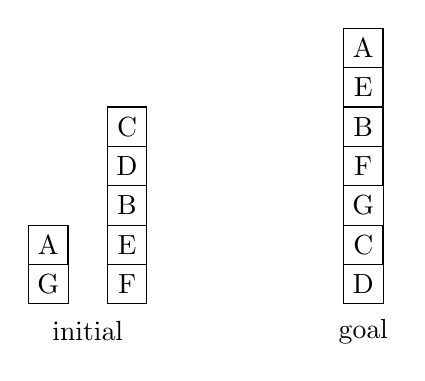
\begin{tikzpicture}
	\node[draw, minimum size=0.5cm] (G) at (0,0) {G};
	\node[draw, minimum size=0.5cm] (A) at (0,0.5) {A};

	\node[draw, minimum size=0.5cm] (F) at (1,0) {F};
	\node[draw, minimum size=0.5cm] (E) at (1,0.5) {E};
	\node[draw, minimum size=0.5cm] (B) at (1,1) {B};
	\node[draw, minimum size=0.5cm] (D) at (1,1.5) {D};
	\node[draw, minimum size=0.5cm] (C) at (1,2) {C};
	\node[] (i) at (0.5,-0.6) {initial};


	\node[draw, minimum size=0.5cm] (D) at (4,0) {D};
	\node[draw, minimum size=0.5cm] (C) at (4,0.5) {C};
	\node[draw, minimum size=0.5cm] (G) at (4,1) {G};
	\node[draw, minimum size=0.5cm] (F) at (4,1.5) {F};
	\node[draw, minimum size=0.5cm] (B) at (4,2) {B};
	\node[draw, minimum size=0.5cm] (E) at (4,2.5) {E};
	\node[draw, minimum size=0.5cm] (A) at (4,3) {A};
	\node[] (g) at (4,-0.6) {goal};
\end{tikzpicture}
\end{center}

MUGS:
\begin{itemize}
	\item $\{on(E,B), on(G,C)\}$
	\item $\{on(A,E), on(C,D), on(G,C)\}$
	\item $\{on(B,F), on(G,C)\}$
	\item $\{on(F,G)\}$
	\item $\{on(A,E), on(C,D), on(E,B)\}$
	\item $\{on(B,F), on(E,B)\}$
	\item $\{on(B,F), on(C,D)\}$
	\item $\{on(A,E), on(B,F)\}$
\end{itemize}




%% \section*{Acknowledgments}
%
%% This material is based upon work supported by the Air Force Office
%% of Scientific Research under award number FA9550-18-1-0245. J\"org
%% Hoffmann's group has also received support by the German Research
%% Foundation (DFG) as part of CRC 248 (see
%% perspicuous-computing.science). Part of this work was performed
%% while J\"org Hoffmann was visiting NASA Ames Research Center.

\bibliographystyle{named}
\bibliography{abbreviations,biblio,crossref}



\end{document}
